\documentclass[12pt]{article}
\usepackage{amsmath}
\usepackage{mathptmx}
\usepackage{setspace}
\usepackage{amssymb}
\usepackage{float}
\usepackage{graphicx}
\usepackage{booktabs}
\usepackage{subfigure}
\usepackage[margin=2.5cm]{geometry}
\usepackage[title]{appendix}
\usepackage{bm}
\usepackage{tcolorbox}
\usepackage{apacite}
\linespread{1.5}
%\usepackage{lineno}
%\linenumbers
\usepackage{diagbox}
\usepackage{longtable}
\usepackage{pdflscape}
\usepackage{rotating}
%\usepackage{subcaption}
%\usepackage{floatrow}
%\usepackage{fontspec}


\DeclareMathOperator*{\argmin}{arg\,min}
\newtheorem{experiment}{Experiment}



\usepackage{fontspec}
\setmainfont{Times New Roman}
\addtolength{\jot}{0.5em}


%\doublespacing
\linespread{2}%1.23

\begin{document}
	
	\begin{titlepage}
		{\centering
%			{\scshape\LARGE Monash University \par}
	%		\vspace{0.5cm}
%			{\scshape\Large Final year project\par}
			\vspace{0.5cm}
			{\huge\bfseries Factor Selection and Factor Strength\\
				\Large An Application to U.S. Stock Market Return\par}
			\vspace{1cm}
			{\Large\itshape Zhiyuan Jiang\\
				I.D: 28710967\par}
			\vfill
			\large supervised by\par
			Dr.~Natalia Bailey\\ Dr.~David Frazier
%			Dr.~Mark \textsc{Brown}
			
			\vspace{1cm}\textbf{Abstract}\par}
%		\noindent\raisebox{.5ex}{\rule{\linewidth}{.4pt}}\par
This section is for the future abstract part.
The abstract length will be controlled within five sentences.
Place Holder.\\
%		\noindent\raisebox{.5ex}{\rule{\linewidth}{.4pt}}\par
		\noindent \textbf{Keywords}: CAPM, Factor Model, Factor Strength, Elastic Net, Lasso
		
		\vfill
		{\centering\large \today\par}
	\end{titlepage}


\section*{Acknoledgements}
I like to acknowledge...





		\pagenumbering{Roman}
\newpage
	\tableofcontents
	\newpage
	\listoffigures
	\listoftables
	\newpage
\setcounter{page}{1}
\pagenumbering{arabic}




\section{Introduction and Motivation}
Capital Asset Pricing Model (CAPM) \cite{Sharpe1964, Lintner1965, Black1972} introduces a risk pricing paradigm.
By incorporating factors, the model divides an asset's risk into two parts: systematic risk and asset specified idiosyncratic risk.
In general, the market factor proxies for the systematic risk, and different risk factors price the idiosyncratic risk.
Researches (see \citeA{Fama1992}, \citeA{Carhart1997}, \citeA{Kelly2019}) have shown that adding different risk factors into the CAPM model can enhance the ability of pricing risk.
Because of this, identifying risk factors has become an important topic in finance.
%Some famous examples of multi-factor CAPM include the Fama-French (FF) three-factor model \cite{Fama1992}, and the Momentum model \cite{Carhart1997}.
% Researchers after them are trying to find new risk factors to include in the multi-factor CAPM model.
Numerous researchers have contributed to this field, and the direct result is an explosive growth of factors.
 \citeA{Harvey2019} have documented and categorised over 500 factors from papers published in the top financial and economic journals, and they find the growth of new factors has sped up since 2008. 
%In his 2011 presidential address, \citeauthor{Cochrane2011} coined the term "factor zoo" to describe the situation factor modelling is facing: researchers and practitioners have too many options when pricing the risk

%In those famous multi-factor model like FF three-factor model \cite{Fama1992}, the loadings of risk factors pass the significant test comfortably, but this is not always the case. 
%But we should notice that not all factors can pass the significance test comfortably every time like the market factor.
But we should notice that for a factor, it may not able to capture the risk-return relationship for every asset.
Therefore, \citeA{Pesaran2019} introduced a new criterion for assessing the significance of each factor, which they call it factor strength.
In general, if a factor can generate coefficients, or refer it as loadings in financial literatures, significantly different from zero for all assets, then we call such a factor strong factor.
%And the less significant loading a factor can generate, the weaker the strength it has.
And the less amounts of significant loadings a factor can generate, the weaker the strength the factor has.

In his 2011 president address \citeauthor{Cochrane2011} emphasized the importance of finding factors which can provide independent information about average return and risk.
With regard to this, many scholars applied various methods to find such factors. 
%Since in their 2015 research \citeA{Harvey2015} argues that the current threshold for a test of parameter significant is too low for newly proposed factors, 
For instance, \citeA{Harvey2017} provided a bootstrap method to adjust the threshold of factor loading's significant test, trying to exclude some falsely significant factor caused by multiple-test problem.
Some other scholars are using machine learning methods to reduce the potential candidates. 
One stream of them has used a shrinkage and subset selection method called Lasso \cite{Tibshirani1996} and it's variations to find suitable factors.
One example of such an application is made by \citeA{Rapach2013}.
They applied the Lasso regression, trying to find some characteristics from a large group to predict the global stock market's return.

But an additional challenge is that factors, especially in the high-dimension, are correlated.
%\citeA{Cochrane2005} argues that the correlation between factors will reduce the ability of using risk premium to infer factors.
\citeA{Kozak2020} point out that when facing a group of correlated factors, Lasso will only pick several highly correlated factors, seemly at random, and then ignore the other and shrink them to zero. 
In other words, Lasso fails to handle the issue of correlated factors appropriately.


%\citeA{Kan1999} found that the test-statistic of FM two-stage regression  \cite{Fama1973} will inflate when incorporating factors which are independent with the cross-section return.
%Provides spurious factors with the chance  to pass the significant test.

%\citeA{Hou2018} found that they can not replicate the result of over 60\% selected factor papers. 

%These discoveries cast doubt on the risk pricing ability of some factors, indicates that some factors may fail to pass the significant test in certain scenarios.

Therefore, the main empirical question in this project is: how to select useful factors from a large group of possibly highly correlated candidates.
We address this question from two different prospects.

From one side, we employ the idea of factor strength discuss above, trying to use this criterion to select those strong factors.
On the other hand, we use another variable selection method called Elastic Net \cite{Zou2005} to select factors.
With regard of the first approach, \citeA{Bailey2020} provide a consistent estimator for the factor strength, and we will use this method to examine the strength of each candidate factor and filter out any spurious factors.
Under the second approach, unlike Lasso, elastic net adds an extra penalty term into the loss function, which makes it suitable to handle the potential correlation variables.
This trait makes it suitable for our purpose.
We will assess and compare the methods in their selection of risk factors.
Additionally, we can also use the factor strength as a standard to reduce the dimension of our candidates factors and then applied the elastic net to conduct further selection.

%First, we consider the selection of factor base on their strength.
%And then we will use another variable selection method called Elastic Net \cite{Zou2005} to select factors.
%With regard of the first stage, \citeA{Bailey2020} provides a consistent estimates method for the factor strength, and we will use such method to exam the strength of each candidate factors, and filter out those spurious factors, therefore,reduce the dimension of the number of potential factors.
%For the second part, elastic net fixes the problem of Lasso can not handle correlated variables by adding extra penalty term, which makes it suitable for our purpose. 

The rest of the thesis is organized as follows.
In section \ref{Literature}, we go through some literatures relate with the CAPM model and methods about factor selection.
Then in section \ref{strength}, we will provide a detailed description of the concept of factor strength and the estimation method.
In section \ref{MC}, we set up a simple Monte Carlo simulation experiment to examine the finite sample properties of the factor strength estimator.
We introduce the elastic net in section \ref{Elastic_Net}.
Section \ref{Empirical} includes the empirical application, where we estimate the strength of potential risk factors to be included in a CAPM model, as well as apply elastic net as a method to select factors.


%For this project, we are trying to deal with the classical problem: what factors can have significant contributions to explain the asset risk and return relationship under the CAPM framework.
%And we go a step forward, take the correlation among all factors into the account. 
%ut before applying the Elastic Net method, we want to first investigate all those factor's strength.
%Our interest is focused on first determine which factors have enough power to help us solve the risk pricing problem. 
%Then, from this pre-determined relatively small factor group, we applied the Elastic Net method, trying to find out the most appropriate factors to help us form the multi-factor CAPM model.



	\section{Related Literature}\label{Literature}
%This project combines three  kinds of literatures: CAPM, factor strength, and factor selection under high dimensioned setting for the number of potential factors.

This project is built on contributions to the field of asset pricing.
First formulated by \citeA{Sharpe1964}, \citeA{Lintner1965}, and \citeA{Black1972}, the original CAPM model only contains the market factor, which is denoted by the difference between average market return and risk-free return.
\citeA{Fama1992} extend the model into three-factors, which it then extend into four \cite{Carhart1997}, and five \cite{Fama2015}.
Recent research created a six-factors model and claim it outperforms all other sparse factor models. \cite{Kelly2019}.

In terms of assessing the strength of risk factors, this thesis also relates to papers discussing factors that have no or weak correlation with assets' return under the paradigm of the CAPM model.
\citeA{Kan1999} found that the test-statistic of FM two-stage regression  \cite{Fama1973} will inflate when incorporating factors which are independent of the cross-section return.
Therefore, when factors with no pricing power were added into the model, those factors may have the chance to pass the significant test falsely.
%\citeA{Kleibergen2009} pointed out how a factor with small loading would deliver a spurious FM two-pass risk premia estimation. 
\citeA{Kleibergen2015} found out that even when some factor-return relationship does not exist, the r-square and the t-statistic of the FM two-stage regression would become in favour of the conclusion of such structure presence. 
\citeA{Gospodinov2017} show how the addition of a spurious factor will distort the statistical inference of parameters.
Besides, \citeA{Anatolyev2018} studied the behaviours of the model with the presence of weak factors under asymptotic settings, and they find the regression will lead to an inconsistent risk premia estimation result.
	
	
Finally, of interest in this thesis is the large dimension of potential factors.
For these reasons, it borrows from researchers that identify useful factors from a group of potential factors.
\citeA{Harvey2015} examine over 300 factors published in journals, presents a new multi testing framework to exam the significance of factors.
And they claim that a higher hurdle for the t-statistic is necessary when examining the significance of newly proposed factors.
%and they suggest to adjust the p-value threshold to around 3. 
Methods like a Bayesian procedure introduced by \citeA{Barillas2018} were used to compare different factor models.
\citeA{Pukthuanthong2019} defined several criteria for "genuine risk factor", and based on those criteria introduced a protocol to examine whether a factor is associated with the risk premium.

%{\bf More details about the previous effort of identifying useful factors }
Once the factor strength is identified, the thesis will attempt to reconcile empirically the factor selection under machine learning techniques and the factor strength implied by the selection.

%This thesis will attempt to address the factor selection problem by using machine learning techniques.
\citeA{Gu2020} elaborate on the advantages of using emerging machine learning algorithms in measuring the equity risk premiums.
They obtained a higher predictive accuracy in measuring risk premium, and demonstrated large economics gains using investment strategy base on the machine learning forecast.
%They found the machine learning method improved the predictive accuracy and provides extra economics gain 
%Those advantages including more accurate prediction result, and superior efficiency.
Various machine learning algorithms have been adopted when selecting factors for the factor model, especially in recent years.
\citeA{Lettau2020} apply Principle Components Analysis when investigating the latent factor of the model. 
Lasso is a popular algorithms for factor selections, because of its ability of selecting features.
%Lasso method, since it's ability to select features, is popular in the field of the factor selection.
\citeA{Feng2019} used the double-selected Lasso method \cite{Belloni2014}, and a grouped lasso method \cite{Huang2010} is used by \citeA{Freyberger2020} when picking factors from a group of candidates. 
\citeA{Kozak2020} arguing that the sparse factor model is ultimately futile by using a Bayesian-based method. 
They constructed their estimator similar to the ridge regressor, but instead of putting the penalty on the sum of squared of factor coefficients, they impose the penalty base on the maximum squared Sharpe ration implied by the factor model.
They also augmented their Bayesian based estimator with extra $L^1$, created a method,  similar but different to the elastic net algorithm which will be employed by our project. (\textbf{Still not very good})

%\documentclass[12pt]{article}
%\usepackage{amsmath}
%\usepackage{mathptmx}
%\usepackage{setspace}
%\usepackage{amssymb}
%\usepackage{float}
%\usepackage{graphicx}
%\usepackage{booktabs}
%\usepackage{subfigure}
%\usepackage[margin=2.5cm]{geometry}
%\usepackage[title]{appendix}
%\usepackage{bm}
%\usepackage{tcolorbox}
%\usepackage{apacite}
%\onehalfspacing
%\usepackage{lineno}
%\linenumbers
%\usepackage{diagbox}

%\usepackage{longtable}
%\usepackage{pdflscape}
%\usepackage{rotating}
%\usepackage{subcaption}
%\usepackage{floatrow}
%\usepackage{fontspec}

%\DeclareMathOperator*{\argmin}{arg\,min}
%\newtheorem{experiment}{Experiment}



%\usepackage{fontspec}
%\setmainfont{Times New Roman}
%\addtolength{\jot}{0.5em}
%\linespread{1.5}




		
%		\begin{document}
\section{Factor Strength}\label{strength}
The concept of factor strength employed in this project comes from \citeA{Bailey2020}, and it was first introduced by \citeA{Bailey2016}.
They defined the strength of factor from prospect of the cross-section dependences of a large panel and connect it to the pervasiveness of the factor, which is captured by the factor loadings.
%The method present in the initial paper focusing the estimation from unobserved factor.
In a separate paper, \citeA{Bailey2019} extended the method by loosen some restrictions, and proved that their estimation can also be applied on the residuals of regression result.
Here, we focus on the case of observed factors, and use the method of \citeA{Bailey2020} in this project.
%Thereafter, they focusing on the case of observed factors, and proposed the method we employed in this project \cite{Bailey2020}.

		\subsection{Definition}\label{strength_definiton}

Consider the following multi-factor model for n different cross-section units and T observations with k  factors.

\[  x_{it} = a_{t}+  \sum_{j=1}^{k}\beta_{ij}f_{jt} + \varepsilon_{it} \tag{1}\label{definition_model} \]
In the left-hand side, we have $x_{it}$ denotes the cross-section unit i at time t, where $i = 1, 2,3, \cdots, n$ and $t = 1,2,3, \cdots T$.  
In the other hand, $a_{i}$ is the constant term.
$f_{jt}$ of $j = 1, 2, 3\cdots k$ is factors included in the model, and $\beta_{ij}$ is the corresponding factor loading.
$\varepsilon_{it}$ is the stochastic error term.

The factor strength is relates to how many non-zero loadings correspond to a factor.
More precisely, for a factor $f_{jt}$ with n different factor loading $\beta_{ij}$, we assume that:
\begin{align*}
|\beta_{ij}| &> 0\quad i = 1, 2,  \dots, [n^{\alpha_j}]\\
|\beta_{ij}| &= 0 \quad i = [n^{\alpha_j}] + 1, [n^{\alpha_j}] +2 ,\dots, n
\end{align*}
The $\alpha_j$ represents strength of factor $f_{jt}$ and $\alpha_j \in [0,1]$.
If factor has strength $\alpha_j$, we will assume that the first $[n^{\alpha_j}]$ loadings are all different from zero, and here $[\cdot] $  is defined as integral operator, which will only take the integral part of inside value.% which indicates that those factors can capture the dynamic behind the cross-section unit effectively.
The rest $n - [n^{\alpha_j}]$ terms are all equal to zero. % which means the factors can not provides any information of interest of  those $n - [n^\alpha_j]$  units.
Assume for a factor which has strength $\alpha = 1$, the factor's loadings will be non-zero for all cross-section units.
We will refer such factor as strong factor.
And if we have factor strength $\alpha = 0$, it means that the factor has all factor loadings equal to zero, and we will describe such factor as weak factor \cite{Bailey2016}.
For any factor with strength in [0.5, 1], we will refer such factor as semi-strong factor.
In general term, the more non-zero loading a factor has, the stronger the factor's strength is. 

	\subsection{Estimation Under single factor setting}\label{strength_one_factor_estimation}
To estimate the strength $\alpha_j$, \citeA{Bailey2020} provides following estimation.

To begin with, we consider a single-factor model with only factor named $f_t$. 
 $\beta_{i}$ is the factor loading of unit i.
$v_{it}$ is the stochastic error term.

\[  x_{it} = a_{i} +  \beta_{i}f_{t} + v_{it} \tag{2} \label{estimation_model}\]

Assume we have n different units and T observations for each unit: $i = 1, 2, 3, \cdots, n$ and $t = 1,2,3, \cdots T$.
Running the OLS regression for each $i = 1,2,3\cdots, n$, we obtain:
\[   x_{it} = \hat{a}_{iT} +  \hat{\beta}_{iT}f_{t} + \hat{v}_{it}  \]

For every factor loading $\hat{\beta}_{iT}$, we can examine their significance by constructing a t-test.
The t-test statistic will be $t_{iT} = \frac{\hat{\beta}_{iT} - 0}{\hat{\sigma}_{iT}}$.  
Then the test statistic for the corresponding $\hat{\beta}_i$ will be:

\[t_{i T}=\frac{\left(\mathbf{f}^{\prime} \mathbf{M}_{\tau} \mathbf{f}\right)^{1 / 2} \hat{\beta}_{i T}}{\hat{\sigma}_{i T}}=\frac{\left(\mathbf{f}^{\prime} \mathbf{M}_{\tau} \mathbf{f}\right)^{-1 / 2}\left(\mathbf{f}^{\prime} \mathbf{M}_{\tau} \mathbf{x}_{i}\right)}{\hat{\sigma}_{i T}} \tag{3} \label{test_statistic} \].
Here, the $\mathbf{M}_{\tau} = \mathbf{I}_T - T^{-1}\mathbf{\tau}\mathbf{\tau^\prime}$, and the $\mathbf{\tau}$ is a $T\times 1$ vector with every elements equals to 1.
$\mathbf{f}$ and $\mathbf{x_i}$ are two vectors with: $\mathbf{f} = (f_1, f_2 \cdots, f_T)^{\prime}$   $\mathbf{x_i} = (x_{i1}, x_{i2}, \cdots, x_{iT})$.
The denominator $\hat{\sigma}_{iT} = \frac{\sum_{i=1}^{T} \hat{v}^2_{it} }{T}$.

Using this test statistic, we can then define an indicator function as: $\ell_{i,n} := {\bf1}[|\beta_i|>0]$.
If the factor loading is non-zero, $\ell_{i,n} = 1$.
In practice, we use the $\hat{\ell}_{i,nT} := {\bf1}[|t_{it}|>c_p(n)]$.
Here, if the t-statistic $t_{iT}$ is greater than critical value $c_p(n)$,  $\hat{\ell}_{i,n} = 1$, otherwise $\hat{\ell}_{i,n} = 0$.
In other words, we are counting how many $\hat{\beta}_{iT}$ are significant.
With the indicator function, we then define $\hat{\pi}_{nT}$ as the fraction of significant factor loading amount to the total factor loadings:

\[  \hat{\pi}_{nT} = \frac{\sum_{i=1}^n \hat{\ell}_{i,nT}}{n} \tag{4} \label{pi_function} \]


In term of the critical value $c_p(n)$, rather than use the traditional critical value from student-t distribution $\Phi^{-1}(1-\frac{P}{2})$, we use:

\[   c_p(n) = \Phi^{-1}(1 - \frac{p}{2n^\delta})   \tag{5} \label{critical_value_function} \]

Suggested by \citeA{Bailey2019}, here, $\Phi^{-1}(\cdot)$ is the inverse cumulative distribution function of a standard normal distribution, p is the size of the test, and $\delta$ is a non-negative value represent the critical value exponent. 
Adopting this adjusted value helps to tackle the problem of multiple-testing.

%This adjusted critical value, adopt helps to tackle the problem of multiple-test.

After obtaining the $\hat{\pi}_{nT}$, we can use the following formula provided by \citeA{Bailey2020} to estimate our strength indicator $\alpha_j$:
\[ \hat{\alpha} = \begin{cases}
1+\frac{\ln(\hat{\pi}_{nT})}{\ln n} & \text{if}\; \hat{\pi}_{nT} > 0,\\
0, & \text{if}\; \hat{\pi}_{nT} = 0.
	\end{cases} \tag{6} \label{estimation_method} \]

Whenever we have $\hat{\pi}_{nT}$, the estimated $\hat{\alpha}$ will be equal to zero. 
From the estimation, we can find out that $\hat{\alpha} \in [0,1]$.

	\subsection{Estimation Under Multi-Factor Setting}\label{strength_multi_estimation}

This estimation can also be extended into a multi-factor set up.
Consider the following multi-factor model:
\[x_{it} = a_i +\sum_{j = 1}^k\beta_{ij}f_{jt} +v_{it} = a_i + \mathbf{\beta^{\prime}_{i}f_{t}} +v_{it} \]

In this set up, we have $i = 1, 2, \cdots, n$ units, $t = 1, 2, \cdots, T$ time observations, and specially, $j = 1, 2,\cdots, k$ different factors.
Here $\mathbf{\beta}_{i} = (\beta_{i1}, \beta_{i2}, \cdots, \beta_{ij})^{\prime} $ and $\mathbf{f}_t = (f_{1t}, f_{2t}\cdots, f_{jt})$.
We employed the same strategy as above, after running OLS and obtain the:

\[ x_{it} =\hat{a}_{iT} + \mathbf{\hat{\beta}_{i}}\mathbf{f}_{t} + \hat{v}_{it}    \]
To conduct the significance test, we calculate the t-statistic: $t_{ijT} = \frac{\hat{\beta}_{ijT}-0}{\hat{\sigma}_{ijT}}$. Empirically, the test statistic can be calculated using:
\[ t_{i j T}=\frac{\left(\mathbf{f}_{j \circ}^{\prime} \mathbf{M}_{F_{-j}} \mathbf{f}_{j \circ}\right)^{-1 / 2}\left(\mathbf{f}_{j \circ}^{\prime} \mathbf{M}_{F_{-j}} \mathbf{x}_{i}\right)}{\hat{\sigma}_{i T}} \]

Here, $\mathbf{f}_{j \circ}=\left(f_{j 1}, f_{j 2}, \ldots, f_{j T}\right)^{\prime}, \mathbf{x}_{i}=\left(x_{i 1}, x_{i 2}, \ldots, x_{i T}\right)^{\prime}, \mathbf{M}_{F_{-j}}=\mathbf{I}-\mathbf{F}_{-j}\left(\mathbf{F}_{-j}^{\prime} \mathbf{F}_{-j}\right)^{-1} \mathbf{F}_{-j}^{\prime}$, and $\mathbf{F}_{-j}=\left(\mathbf{f}_{1 \circ}, \ldots, \mathbf{f}_{j-1 \circ}, \mathbf{f}_{j+1 \circ}, \ldots, \mathbf{f}_{m \circ}\right)^{\prime}$
For the denominator's $\hat{\sigma}_{iT}$, it was from $\hat{\sigma}_{i T}^{2}=T^{-1} \sum_{t=1}^{T} \hat{u}_{i t}^{2}$, the $\hat{u}_{it}$ is the residuals of the model.
Then, we can use the same critical value from (\ref{critical_value_function}).
Obtaining the corresponding ratio $\hat{\pi}_{nTj}$  from (\ref{pi_function}), and use the function:
\begin{equation*}
\hat{\alpha}_{j}=\left\{\begin{array}{l}
1+\frac{\ln \hat{\pi}_{n T, j}}{\ln n}, \text { if } \hat{\pi}_{n T, j}>0 \\
0, \text { if } \hat{\pi}_{n T, j}=0
\end{array}\right.
\end{equation*}
to estimate the factor strength.


%+==================+==================+==================+===============&
%+==================+==================+==================+===============&

	\section{Monte Carlo Design}\label{MC}
	\subsection{Design}
In order to study the finite sample properties of factor strength $\hat{\alpha}_j$, we conduct a Monte Carlo study.
Through the simulation, we compare the property of the factor strength in different settings.
We set up the experiments to reflect the CAPM model and its extension.
For simplicity, we first define $x_{it} := r_{it}- r_{ft}$.
$r_{it}$ is the unit's return, and $r_{ft}$ represent the risk-free rate at time t, therefore, the $x_{it}$ is the excess return of unit i at time t.
We use $f_{mt}:=r_{mt} - r_{ft}$ to denote the market factor.
Here $r_{mt}$ is the average market return of hypothetically all assets in the universe.
Additionally, we set $q_1(\cdot)$ and $q_2(\cdot)$ as two different functions that represent the unknown mechanism of market factor and other risk factors in pricing asset risk.
In the classical CAPM model and it's multi-factor extensions, for example, the three-factor model introduced by \citeA{Fama1992}, both $q_1$ and $q_2$ are linear.
Now consider the following data generating process (DGP):

%	\[ r_{it} - r_{ft} = q_1({r_{mt}} - r_f) + q_2( \sum_{j=1}^k\beta_{ij}f_{jt}) +\epsilon_{it} \]
	
	\[ x_{it} = q_1(f_{mt}) + q_2( \sum_{j=1}^k\beta_{ij}f_{jt}) +\epsilon_{it}  \]


In the simulation, we consider a dataset has $i = 1, 2,\dots, n$ different cross-section units, with $t= 1, 2,\dots, T$ different observations. 
%$r_{it}$ is the unit's return, and $r_{ft}$ represent the risk-free rate at time t, therefore, the left-hand side term $r_{it} - r_{ft}$ is the excess return of unit i.
%For simplicity, we define $x_{it} := r_{it}- r_{ft}$.
$f_{jt}$ represents different risk factors, and the corresponding  $\beta_{ij}$ are the factor loadings.
%We use $f_{mt}:=r_{mt} - r_{ft}$ to denote the market factor, and here $r_{mt}$ is the average market return.
%Also, we use the term $f_{mt} := r_{mt} - r_{ft}$ to denotes the market factor.
We expect the market factor will have strength equal to one all the time, so we consider the market factor has strength $\alpha_m = 1$.
$\varepsilon_{it}$ is the stochastic error term.
%Therefore, the simulation model can be simplified as:

%\[ x_{it} = q_1(f_{mt}) + q_2( \sum_{j=1}^k\beta_{ij}f_{jt}) +\epsilon_{it}  \]

%$q_1(\cdot)$ and $q_2(\cdot)$ are two different functions that represent the unknown mechanism of market factor and other risk factors in pricing asset risk.
%In the classical CAPM model and it's multi-factor extensions, for example, the three-factor model introduced by \citeA{Fama1992}, both $q_1$ and $q_2$ are linear.

 For each factor, we assume they follow a multivariate normal distribution with mean zero and a $k\times k$ variance-covariance matrix $\Sigma$. 
\begin{align*}
\mathbf{f_t} = \begin{pmatrix}
f_{i,t}\\f_{2,t}\\\vdots\\f_{k,t}
\end{pmatrix} \sim MVN(\mathbf{0}, \Sigma) \quad
 \Sigma := 
\begin{pmatrix}
\sigma^2_{f_1}, & \rho_{12}\sigma_{f1}\sigma_{f2} &\cdots  & \rho_{1k}\sigma_{f1}\sigma_{fk}\\
\rho_{12}\sigma_{f2}\sigma_{f1}, & \sigma^2_{f2} &\cdots  & \rho_{2k}\sigma_{f2}\sigma_{fk}\\
\vdots & \vdots & \ddots & \vdots \\
\rho_{1k}\sigma_{fk}\sigma_{f1}, & \rho_{k2}\sigma_{fk}\sigma_{f2} &\cdots  & \sigma^2_{fk}\\
\end{pmatrix}
\end{align*}
The diagonal of matrix $\Sigma$ indicates the variance of each factor, and the rest represent the covariance among all $k$ factors.


	\subsection{Experiment Setting}\label{exp_set}



%\subsection{Baseline Experiment}\label{base}
Follow the general model above, we assume both $q_1(\cdot)$ and $q_2(\cdot)$ are linear function:
\begin{align*}
q_1({f_{mt}}) &= a_{i} +\beta_{im} f_{mt}\\
q_2(\sum_{j = 1}^{k}\beta_{ij}f_{jt}) &=\sum_{j = 1}^{k}\beta_{ij}f_{jt}
\end{align*}
To start the simulation, we consider a two-factor model:
\[    x_{it} = a_{i} + \beta_{i1}f_{1t} + \beta_{i2}f_{2t}+\epsilon_{it} \tag{7} \label{two_factor}   \]
%Therefore, if we include the market factor with other risk factors together, the model can be simplified as:
%	\[   x_{it} = a_{it} + \sum_{j = 1}^{k+1}  \beta_{ij}f_{jt} +\epsilon_{it}  \tag{6} \label{simplified_multi}  \x]
%And in this first baseline experiment, we will  use the single factor model as:
%\[  x_{it} = a_{it} +  \beta_{i1}f_{1t} +\epsilon_{it} \tag{7} \label{singlefactor}  \]
%Through the simulations, we will control the underlying true strength of factor 
The constant term $a_{i}$ is generated from a uniform distribution, $a_{it} \sim \mathnormal{U}[-0.5,0.5]$.
For the factor loading $\beta_{i1}$ and $\beta_{i2}$, we first use a uniform distribution $IIDU(\mu_{\beta} - 0.2, \mu_{\beta}+0.2)$ to produce the values.
Here we set $\mu_{\beta}=0.71$ to make sure every generated loading value is sufficiently larger than 0.
Then we randomly assign $n - [n^{\alpha_{1}}]$ and $n - [n^{\alpha_{2}}]$ factor loadings as zero.
$\alpha_1$ and $\alpha_2$ are the true factor strength of $f_1$ and $f_2$. 
In this simulation, we will start the factor strength from 0.7 and increase it gradually till unity with pace 0.05, say $(\alpha_{1}, \alpha_{2}) = \{0.7, 0.75,0.8,\cdots,1\}$.
 $[\cdot]$ is the integer operator defined at section (\ref{strength_one_factor_estimation}).
This step reflects the fact that only $[n^\alpha_1]$ or $[n^\alpha_2]$ factor loadings are non-zero.
In terms of the factors, they come from a multinomial distribution $MVN(\mathbf{0}, \Sigma) $, as we discuss before.

Currently, we consider three different experiments set up:

\begin{experiment}[single factor, normal error, no correlation]
Set $\beta_{i2}$ from (\ref{two_factor}) as 0, the error term $\varepsilon_{it}$ and the factor $f_{1t}$ are both standard normal.
\end{experiment}

\begin{experiment}[two factors, normal error, no correlation]
Both $\beta_{i1}$ and $\beta_{i2}$ are non-zero. Error term and both factors are standard normal. The correlation $\rho_{12}$ between $f_{1t}$ and$f_{2t}$ is zero. 
The factor strength for the first factor $\alpha_1 = 1$ all the time, and $\alpha_2$ varies.
\end{experiment}

\begin{experiment}[two factors, normal error, weak correlation]
Both $\beta_{i1}$ and $\beta_{i2}$ are non-zero. Error term  and both factors are standard normal. The correlation $\rho_{12}$ between $f_{1t}$ and$f_{2t}$ is 0.3.
The factor strength for the first factor $\alpha_1 = 1$ all the time, and $\alpha_2$ varies.
\end{experiment}

The factor strength in each experiment is estimated using the method discussed in section (\ref{strength_one_factor_estimation}), the size of the significance test is $p = 0.05$, and the critical value exponent $\sigma$ has been set as 0.5.
For each experiment, we calculate the bias, the RMSE and the size of the test to assess the estimation performances.
The bias is calculated as the difference between the true factor strength $\alpha$ and the estimated factor strength $\hat{\alpha}$.
\[bias = \alpha - \hat{\alpha}\]
The Root Square Mean Error (RMSE) comes from:
\[ RMSE =[\frac{1}{R}\sum_{r=1}^{R}(bias_r)^2 ]^{1/2}\]
Where the R represents the total number of replication.
The size of the test is under the hypothesis that $H_0: \hat{\alpha_j} = \alpha_j,\;j =1, 2$ against the alternative hypothesis $H_1:\hat{\alpha_j} \neq \alpha_j,\; j=1,2$.
Here we employed the following test statistic from \citeA{Bailey2020}.

	\[  z_{\hat{\alpha_j}:\alpha_j} =\frac{(\ln n)\left(\hat{\alpha_j}-\alpha_{j}\right)-p\left(n-n^{\hat{\alpha_j}}\right) n^{-\delta-\hat{\alpha_j}}}{\left[p\left(n-n^{\hat{\alpha}_j}\right) n^{-\delta-2 \hat{\alpha}_j}\left(1-\frac{p}{n^{\delta}}\right)\right]^{1 / 2}}\quad j=1,2 \tag{8}  \label{z_indicator}\]

Define a indicator function $\mathbf{1}(|z_{\hat{\alpha_j}:\alpha_j} |>c|H_0)$.
For each replication, if this test statistic is greater than the critical value of standard normal distribution: $c = 1.96$, the indicator function will return value 1, and 0 otherwise.
Therefore, we calculate the size of the test base on:
	\[ size = \frac{\sum_{r=1}^{R} \mathbf{1}(|z_{\hat{\alpha_j}:\alpha_j} |>1.96|H_0)}{R} \quad j =1,2 \tag{9}, \label{size_calculator}\]

%Next, we set up the true factor strength $\alpha$.
%Through the whole simulation, we will assign the strength with different value $\alpha = \{0.5, 0.7, 0.9, 1\}$, and since in this baseline design we only contain one factor, the only factor's strength will be selected from the above set. 
%After having the factor strength, we can calculate for each factor, how many loadings should be different from zero.
%From the section (\ref{definiton}), we assume that for any factor with strength $\alpha_j$, the factor is supposed to generate $[n^{\alpha_j}]$ non-zero factor loadings, and $n- [n^{\alpha_j}]$ zero loadings.
%Therefore, we can calculate the $n - [n^{\alpha_j}]$.

%From the previous section, we assume factors will follow a multinomial standard distribution with mean zero and variance $\Sigma$.
%This means that for each factors, they should follow a normal distribution.
%In this baseline design, we only contain one factor, and this factor will generate form standard error distribution.


%For this experiment, we construct the hypothesis test base on the null hypothesis $H_O:\beta_{i1} = 0$ against the alternative hypothesis $H_1:\beta_{i1}\neq0$.
%The  test statistic and critical value are from equation (\ref{test_statistic}) and equation (\ref{critical_value_function}).
%We consider two-sided tests, with size 0.05.
%Therefore, the corresponding critical value for such t-test will be $\delta = 1.96$

%After generate constant term, factor, factor loading, and the error term, we can calculate the simulated asset's return by using the equation (\ref{singlefactor}).
%With the return and factors, we can re-calculate the factors loading and use the estimation method discussed in section \ref{estimation}.



%\subsection{Two factor experiment}
%Follow the similar idea as baseline design, we can easily extend the DGP into multi-factor form. 
%We derive a two-factor model from the model  (\ref{simplified_multi}).
%	\[   x_{it} = a_{it} + \beta_{i1}f_{1t} + \beta_{i2}f_{2t}+\epsilon_{it}  \tag{8}  \]
%Here $\mathbf{f}_t = (f_{1t}, f_{2t})^{\prime}$ are two different factors generate from multivariate normal distribution with mean zero and variance $\Sigma$.
%In this simulation, we assume two factors are independent with each other and both of them have variance equals to one, the variance-covariance matrix $\Sigma$ of factors %$\mathbf{f_t}$ will be:
%\begin{align*}
%\Sigma_{\mathbf{f_t}} := 
%\begin{pmatrix}
%1 &0\\
%0 & 1 \\
%\end{pmatrix}
%\end{align*}
%Besides, for the factor $f_{1t}$, we assign it as the market factor, which indicates that the factor strength $\alpha_1$ will be unit.
%And all factor loading generates from this factor will be different from zero.
%For the rest of the variables, we follow the same procedure as the baseline experiment.

In purpose of Monte Carlo Simulation, we consider the different combinations of T and n with $T = \{120, 240, 360\}$, $n =\{100, 300, 500\} $.
The market factor will have strength $\alpha_m = 1$ all the time, and the strength of the other factor will be $\alpha_{x} = \{0.7, 0.75, 0.8,0.85, 0.9,0.95, 1\}$. For every setting, we will replicate 2000 times independently, all the constant and variables will be re-generated for each replication.


 
\subsection{Monte Carlo Results}
We report the results in Table (\ref{table:exp1}), (\ref{table:exp2}) and (\ref{table:exp3}) in Appendix \ref{simulationtable}.

Table (\ref{table:exp1}) provides the results under the experiment 1.
The estimation method we applied tends to over-estimate the strength slightly most of the time when the true strength is relatively weak under the single factor set up.
With the strength increasing, the bias will turn to negative, represents an under-estimated results.
Such bias, however, vanishes quickly while observation t, unit amount n, and true strength $\alpha$ increase.
When we increase the time spam by including more data from the time dimensions, the bias, as well as the RMSE decrease significantly.
Also, when including more cross-section unit n into the simulation, the performance of the estimation improves, as shown by the decreased bias and RMSE values.
An impressive result is that the gap between estimation and true strength will go to zero when we have $\alpha = 1$, the strongest strength we can have.
With the strength approaching unity, both bias and RMSE will converge to zero.
We also present the size of the test in the table.
The size of the test will not vary too much when the strength increases, so as the unit increases,
But we can observe that when observations for each unit increase, in other words, when t increases, the size will shrink dramatically.
The size will become smaller than the 0.05 threshold after we extend the t to 240, or empirically speaking, when we included 20 years monthly return data into the estimation.
Notice that, from the equation (\ref{z_indicator}), when $\hat{\alpha} = \alpha = 1$, the nominator becomes zero.
Therefore, the size will collapse to zero in all settings, so we do not report the size for $\hat{\alpha} = \alpha = 1$

For the two factors scenarios, we obtain similar conclusions in both the no correlation setting and weak correlation setting.
The result of no correlation settings is shown in the table (\ref{table:exp2}), and the table (\ref{table:exp3}) shows the result when the correlation between two factors is 0.3.
%Same as the single factor results, in most of the time, our estimation method will slightly under estimates the factor strength. 
The estimation results improve when increasing either the observations amount t, or the cross-section units amount n.
We also have the same unbiased estimation when true factor strength is unity under all unit-time combinations.
In some cases, even when the factor strength is relatively weak, we can have unbiased estimation if the n and t are big enough. (see table (\ref{table:exp3})).
However, we should also notice that when t > n, the results of the size of the test in two factors setting are performing similar to the single factor result. 
The size will shrink with the observation amount t increasing, and when we have t greater than 240, the size will be smaller than 0.05 threshold in all situations.

%Same results are found in the two factors experiments.
%Table (\ref{exp2_table}) and Table (\ref{exp3_table}) shows the result of experiment 2 and 3.
%With regard of the correlation $\rho_{12}$ between factors, we found that for either cases the  $\rho{12} = 0$ or $\rho_{12} = 0.3$, the bias and RMSE will decrease gradually till converge to zero when the true strength is approaching unity.

%\newpage
%\bibliographystyle{apacite}
%\bibliography{thesis.bib}

%\newpage
%\appendix
%%\documentclass[12pt]{article}
%\usepackage{amsmath}
%\usepackage{mathptmx}
%\usepackage{setspace}
%\usepackage{amssymb}
%\usepackage{float}
%\usepackage{graphicx}
%\usepackage{booktabs}
%\usepackage{subfigure}
%\usepackage[margin=2.5cm]{geometry}
%\usepackage[title]{appendix}
%\usepackage{bm}
%\usepackage{tcolorbox}
%\usepackage{apacite}
%\onehalfspacing

%

%\begin{document}

	
	\section{Simulation Result}\label{simulationtable}
\begin{table}[!hbt]
		\caption{Simulation result for single factor setting}\label{table:exp1}
	\centering

	\begin{tabular}{lccccccccc}
		\hline
		\hline
		\multicolumn{1}{l|}{}                   & \multicolumn{9}{c}{Single Factor}                                                               \\ \hline
		\multicolumn{1}{l|}{}                   & \multicolumn{3}{c|}{Bias $\times$ 100}        & \multicolumn{3}{c|}{RMSE $\times$ 100}     & \multicolumn{3}{c}{Size $\times$ 100} \\ \hline
		\multicolumn{10}{c}{$\alpha_1 = 0.7$}                                                                                                                            \\ \hline
		\multicolumn{1}{l|}{n\textbackslash{}T} & 120    & 240    & \multicolumn{1}{c|}{360}    & 120   & 240   & \multicolumn{1}{c|}{360}   & 120         & 240         & 360        \\ \hline
		\multicolumn{1}{l|}{100}                & 0.256  & 0.265  & \multicolumn{1}{c|}{0.227}  & 0.612 & 0.623 & \multicolumn{1}{c|}{0.560} & 7.85        & 7.7         & 5.55       \\
		\multicolumn{1}{l|}{300}                & 0.185  & 0.184  & \multicolumn{1}{c|}{0.184}  & 0.363 & 0.338 & \multicolumn{1}{c|}{0.335} & 8.9         & 4.45        & 4.5        \\
		\multicolumn{1}{l|}{500}                & 0.107  & 0.124  & \multicolumn{1}{c|}{0.109}  & 0.259 & 0.248 & \multicolumn{1}{c|}{0.234} & 6.9         & 2.5         & 1.6        \\ \hline
		\multicolumn{10}{c}{$\alpha_1 = 0.75$}                                                                                                                          \\ \hline
		\multicolumn{1}{c|}{100}                & -0.178 & -0.159 & \multicolumn{1}{c|}{-0.168} & 0.490 & 0.465 & \multicolumn{1}{c|}{0.450} & 2.5         & 0.85        & 0.4        \\
		\multicolumn{1}{l|}{300}                & 0.154  & 0.156  & \multicolumn{1}{c|}{0.143}  & 0.281 & 0.258 & \multicolumn{1}{c|}{0.234} & 9.4         & 3.7         & 3.35       \\
		\multicolumn{1}{l|}{500}                & 0.024  & 0.033  & \multicolumn{1}{c|}{0.263}  & 0.171 & 0.155 & \multicolumn{1}{c|}{0.148} & 7.8         & 2           & 1.25       \\ \hline
		\multicolumn{10}{c}{$\alpha_1 = 0.8$}                                                                                                                           \\ \hline
		\multicolumn{1}{l|}{100}                & -0.270 & -0.265 & \multicolumn{1}{c|}{-0.258} & 0.434 & 0.409 & \multicolumn{1}{c|}{0.411} & 71.4        & 72.05       & 71.45      \\
		\multicolumn{1}{l|}{300}                & -0.052 & -0.044 & \multicolumn{1}{c|}{-0.043} & 0.183 & 0.149 & \multicolumn{1}{c|}{0.150} & 10.15       & 2.45        & 2.9        \\
		\multicolumn{1}{l|}{500}                & 0.045  & 0.068  & \multicolumn{1}{c|}{0.067}  & 0.136 & 0.126 & \multicolumn{1}{c|}{0.121} & 16.6        & 6.4         & 5.9        \\ \hline
		\multicolumn{10}{c}{$\alpha_1 = 0.85$}                                                                                                                          \\ \hline
		\multicolumn{1}{l|}{100}                & 0.053  & 0.062  & \multicolumn{1}{c|}{0.058}  & 0.253 & 0.228 & \multicolumn{1}{c|}{0.221} & 6.05        & 2.95        & 2.5        \\
		\multicolumn{1}{l|}{300}                & -0.012 & 0.009  & \multicolumn{1}{c|}{-0.001} & 0.124 & 0.104 & \multicolumn{1}{c|}{0.095} & 10.55       & 1.8         & 1.15       \\
		\multicolumn{1}{l|}{500}                & -0.026 & -0.007 & \multicolumn{1}{c|}{-0.011} & 0.096 & 0.073 & \multicolumn{1}{c|}{0.069} & 13.25       & 0.9         & 0.7        \\ \hline
		\multicolumn{10}{c}{$\alpha_1 = 0.9$}                                                                                                                           \\ \hline
		\multicolumn{1}{l|}{100}                & 0.025  & 0.038  & \multicolumn{1}{c|}{0.360}  & 0.191 & 0.163 & \multicolumn{1}{c|}{0.157} & 6.85        & 2           & 1.65       \\
		\multicolumn{1}{l|}{300}                & -0.034 & -0.018 & \multicolumn{1}{c|}{-0.020} & 0.099 & 0.069 & \multicolumn{1}{c|}{0.068} & 13.2        & 0.8         & 0.9        \\
		\multicolumn{1}{l|}{500}                & -0.025 & -0.001 & \multicolumn{1}{c|}{-0.001} & 0.072 & 0.044 & \multicolumn{1}{c|}{0.044} & 22.3        & 1.95        & 1.8        \\ \hline
		\multicolumn{10}{c}{$\alpha_1 = 0.95$}                                                                                                                          \\ \hline
		\multicolumn{1}{l|}{100}                & -0.099 & -0.088 & \multicolumn{1}{c|}{-0.090} & 0.156 & 0.125 & \multicolumn{1}{c|}{0.126} & 5.6         & 0.3         & 0.55       \\
		\multicolumn{1}{l|}{300}                & -0.046 & -0.025 & \multicolumn{1}{c|}{-0.026} & 0.083 & 0.045 & \multicolumn{1}{c|}{0.045} & 22.5        & 2.2         & 2.25       \\
		\multicolumn{1}{l|}{500}                & -0.030 & -0.006 & \multicolumn{1}{c|}{-0.006} & 0.061 & 0.026 & \multicolumn{1}{c|}{0.025} & 33.1        & 4.4         & 3.8        \\ \hline
		\multicolumn{10}{c}{$\alpha_1=1$}                                                                                                                               \\ \hline
		\multicolumn{1}{l|}{100}                & 0      & 0      & \multicolumn{1}{c|}{0}      & 0     & 0     & \multicolumn{1}{c|}{0}     & -           & -           & -          \\
		\multicolumn{1}{l|}{300}                & 0      & 0      & \multicolumn{1}{c|}{0}      & 0     & 0     & \multicolumn{1}{c|}{0}     & -           & -           & -          \\
		\multicolumn{1}{l|}{500}                & 0      & 0      & \multicolumn{1}{c|}{0}      & 0     & 0     & \multicolumn{1}{c|}{0}     & -           & -           & -          \\ \hline
\hline
\end{tabular}
\bigskip\\
{\bf Notes:}
This table shows the result of  experiment 1.
Factors and error are generate from standard normal distribution.
Factor loadings come form uniform distribution $IIDU(\mu_{\beta} - 0.2, \mu_{\beta}+0.2)$, and $\mu_{\beta} = 0.71$.
We keep  $[n^{\alpha_{j}}]$ amount of loadings and assign the rest as zero.
For each different time-unit combinations, we replicate 2000 times.
For the size of the test, we use a two-tail test, under the hypothesis of $H_0, \hat{\alpha}_j = \alpha_j\; j=1,2$.
Cause under the scenarios of $\alpha = 1$, the size of the test will collapse, therefore the table does not report the sizes for $\alpha_1 = 1$.
\end{table}


\begin{table}[!hbt]
		\caption{Simulation result for double factors setting (no correlation)}\label{table:exp2}
	\centering
	\begin{tabular}{lccccccccc}
		\hline
		\hline
\multicolumn{1}{l|}{}                   & \multicolumn{9}{c}{Double Factor with correlation $\rho_{12} = 0$}                                                                \\ \hline
\multicolumn{1}{l|}{}                   & \multicolumn{3}{c|}{Bias $\times$ 100}        & \multicolumn{3}{c|}{RMSE $\times$ 100}      & \multicolumn{3}{c}{Size $\times$ 100} \\ \hline
\multicolumn{10}{c}{$\alpha_1 = 1, \alpha_2  = 0.7$}                                                                                                                           \\ \hline
\multicolumn{1}{l|}{n\textbackslash{}T} & 120    & 240    & \multicolumn{1}{c|}{360}    & 120    & 240   & \multicolumn{1}{c|}{360}   & 120         & 240        & 360         \\ \hline
\multicolumn{1}{l|}{100}                & 0.567  & 0.737  & \multicolumn{1}{c|}{0.628}  & 4.062  & 3.819 & \multicolumn{1}{c|}{3.799} & 2.95        & 1.45       & 1.85        \\
\multicolumn{1}{l|}{300}                & 0.512  & 0.611  & \multicolumn{1}{c|}{0.518}  & 2.398  & 2.103 & \multicolumn{1}{c|}{1.979} & 6.25        & 0.55       & 0.5         \\
\multicolumn{1}{l|}{500}                & -0.149 & 0.08   & \multicolumn{1}{c|}{-0.019} & 1.796  & 1.498 & \multicolumn{1}{c|}{1.443} & 8           & 0.2        & 0.1         \\ \hline
\multicolumn{10}{c}{$\alpha_1 = 1, \alpha_2 =0.75$}                                                                                                                              \\ \hline
\multicolumn{1}{c|}{100}                & -3.051 & -3.02  & \multicolumn{1}{c|}{-3.092} & 4.582  & 4.245 & \multicolumn{1}{c|}{4.248} & 2.45        & 0.1        & 0.10        \\
\multicolumn{1}{l|}{300}                & 0.491  & -1.035 & \multicolumn{1}{c|}{0.640}  & 1.843  & 1.460 & \multicolumn{1}{c|}{1.576} & 7.6         & 0.8        & 0.55        \\
\multicolumn{1}{l|}{500}                & -0.611 & -0.372 & \multicolumn{1}{c|}{-0.393} & 1.520  & 1.136 & \multicolumn{1}{c|}{1.125} & 11.35       & 0.15       & 0.1         \\ \hline
\multicolumn{10}{c}{$\alpha _1= 1, \alpha_2 = 0.8$}                                                                                                                              \\ \hline
\multicolumn{1}{l|}{100}                & -3.752 & -3.630 & \multicolumn{1}{c|}{-3.581} & 4.557  & 4.213 & \multicolumn{1}{c|}{4.210} & 84.65       & 85.9       & 85.25       \\
\multicolumn{1}{l|}{300}                & -1.218 & -0.331 & \multicolumn{1}{c|}{-1.021} & 1.812  & 0.792 & \multicolumn{1}{c|}{1.438} & 9.35        & 0.2        & 0.3         \\
\multicolumn{1}{l|}{500}                & -0.022 & 0.192  & \multicolumn{1}{c|}{0.147}  & 1.047  & 0.782 & \multicolumn{1}{c|}{0.742} & 15.35       & 1.1        & 1.1         \\ \hline
\multicolumn{10}{c}{$\alpha_1 = 1, \alpha_2 = 0.85$}                                                                                                                             \\ \hline
\multicolumn{1}{l|}{100}                & -0.075 & 0.127  & \multicolumn{1}{c|}{0.088}  & 1.996  & 1.697 & \multicolumn{1}{c|}{1.606} & 5.4         & 1.15       & 0.95        \\
\multicolumn{1}{l|}{300}                & -0.531 & -0.406 & \multicolumn{1}{c|}{-0.351} & 1.097  & 0.613 & \multicolumn{1}{c|}{0.777} & 10.8        & 0.15       & 0.2         \\
\multicolumn{1}{l|}{500}                & -0.647 & -0.391 & \multicolumn{1}{c|}{-0.391} & 1.020  & 0.643 & \multicolumn{1}{c|}{0.630} & 19.1        & 0.15       & 0           \\ \hline
\multicolumn{10}{c}{$\alpha_1 = 1, \alpha_2 = 0.9$}                                                                                                                              \\ \hline
\multicolumn{1}{l|}{100}                & -0.128 & 0.043  & \multicolumn{1}{c|}{0.025}  & 1.428  & 1.143 & \multicolumn{1}{c|}{1.118} & 4.9         & 0.65       & 0.7         \\
\multicolumn{1}{l|}{300}                & -0.651 & -0.334 & \multicolumn{1}{c|}{-0.394} & 1.002  & 0.435 & \multicolumn{1}{c|}{0.617} & 17.1        & 0.6        & 0.2         \\
\multicolumn{1}{l|}{500}                & -0.434 & -0.168 & \multicolumn{1}{c|}{-0.171} & 0.7435 & 0.367 & \multicolumn{1}{c|}{0.368} & 25.2        & 0.4        & 0.3         \\ \hline
\multicolumn{10}{c}{$\alpha_1 = 1, \alpha_2 = 0.95$}                                                                                                                             \\ \hline
\multicolumn{1}{l|}{100}                & -1.218 & -1.043 & \multicolumn{1}{c|}{-1.036} & 1.603  & 1.222 & \multicolumn{1}{c|}{1.212} & 6.65        & 0.25       & 0.05        \\
\multicolumn{1}{l|}{300}                & -0.611 & -0.344 & \multicolumn{1}{c|}{-0.356} & 0.881  & 0.435 & \multicolumn{1}{c|}{0.434} & 23.35       & 0.6        & 0.45        \\
\multicolumn{1}{l|}{500}                & -0.415 & -0.123 & \multicolumn{1}{c|}{-0.134} & 0.661  & 0.220 & \multicolumn{1}{c|}{0.216} & 36.75       & 1.35       & 1.1         \\ \hline
\multicolumn{10}{c}{$\alpha_1=1, \alpha_2 = 1$}                                                                                                                                  \\ \hline
\multicolumn{1}{l|}{100}                & 0      & 0      & \multicolumn{1}{c|}{0}      & 0      & 0     & \multicolumn{1}{c|}{0}     & -           & -          & -           \\
\multicolumn{1}{l|}{300}                & 0      & 0      & \multicolumn{1}{c|}{0}      & 0      & 0     & \multicolumn{1}{c|}{0}     & -           & -          & -           \\
\multicolumn{1}{l|}{500}                & 0      & 0      & \multicolumn{1}{c|}{0}      & 0      & 0     & \multicolumn{1}{c|}{0}     & -           & -          & -           \\ \hline\hline
	\end{tabular}
\bigskip\\
{\bf Notes:}
This table shows the result of  experiment 2.
Factors and errors are generate from standard normal distribution.
Between two factors, we assume they have no correlation.
Factor loadings come form uniform distribution $IIDU(\mu_{\beta} - 0.2, \mu_{\beta}+0.2)$, and $\mu_{\beta}$ is set to 0.71.
We keep  $[n^{\alpha_{j}}]$ amount of loadings and assign the rest as zero.
For each different time-unit combinations, we replicate 2000 times.
For the size of the test, we use a two-tail test, under the hypothesis of $H_0, \hat{\alpha}_j = \alpha_j\; j=1,2$.
Cause under the scenarios of $\alpha = 1$, the size of the test will collapse, therefore the table does not report the sizes for $\alpha_1 = \alpha_2 = 1$
\end{table}


	\begin{table}[]
		\caption{Simulation result for double factors setting (weak correlation)}\label{table:exp3}
		\centering
	\begin{tabular}{lccccccccc}
		\hline
		\hline
		\multicolumn{1}{l|}{}                   & \multicolumn{9}{c}{Double Factor with correlation $\rho_{12} = 0.3$}                                                               \\ \hline
		\multicolumn{1}{l|}{}                   & \multicolumn{3}{c|}{Bias $\times$ 100}        & \multicolumn{3}{c|}{RMSE $\times$ 100}     & \multicolumn{3}{c}{Size $\times$ 100} \\ \hline
		\multicolumn{10}{c}{$\alpha_1 = 1, \alpha_2 = 0.7$}                                                                                                                            \\ \hline
		\multicolumn{1}{l|}{n\textbackslash{}T} & 120    & 240    & \multicolumn{1}{c|}{360}    & 120   & 240   & \multicolumn{1}{c|}{360}   & 120          & 240        & 360        \\ \hline
		\multicolumn{1}{l|}{100}                & 0.038  & 0.064  & \multicolumn{1}{c|}{0.072}  & 0.421 & 0.382 & \multicolumn{1}{c|}{0.389} & 4.6          & 1.75       & 1.95       \\
		\multicolumn{1}{l|}{300}                & 0.021  & 0.058  & \multicolumn{1}{c|}{0.056}  & 0.253 & 0.206 & \multicolumn{1}{c|}{0.198} & 9.95         & 0.9        & 0.25       \\
		\multicolumn{1}{l|}{500}                & -0.032 & 0.006  & \multicolumn{1}{c|}{0}      & 0.201 & 0.153 & \multicolumn{1}{c|}{0}     & 12.20        & 0.1        & 0.05       \\ \hline
		\multicolumn{10}{c}{$\alpha_1 = 1, \alpha_2 = 0.75$}                                                                                                                          \\ \hline
		\multicolumn{1}{c|}{100}                & -0.325 & -0.313 & \multicolumn{1}{c|}{-0.310} & 0.488 & 0.419 & \multicolumn{1}{c|}{0.420} & 4.75         & 0.1        & 0          \\
		\multicolumn{1}{l|}{300}                & 0.028  & 0.063  & \multicolumn{1}{c|}{0.065}  & 0.253 & 0.157 & \multicolumn{1}{c|}{0.159} & 9.95         & 0.55       & 0.5        \\
		\multicolumn{1}{l|}{500}                & -0.082 & -0.037 & \multicolumn{1}{c|}{-0.039} & 0.175 & 0.114 & \multicolumn{1}{c|}{0.112} & 19.25        & 0.25       & 0.3        \\ \hline
		\multicolumn{10}{c}{$\alpha_1 = 1, \alpha_2 = 0.8$}                                                                                                                           \\ \hline
		\multicolumn{1}{l|}{100}                & -0.393 & -0.361 & \multicolumn{1}{c|}{-0.368} & 0.477 & 0.418 & \multicolumn{1}{c|}{0.421} & 85.45        & 85.2       & 86.4       \\
		\multicolumn{1}{l|}{300}                & 0.029  & -0.099 & \multicolumn{1}{c|}{-0.100} & 0.192 & 0.145 & \multicolumn{1}{c|}{0.145} & 12.2         & 0.65       & 0.5        \\
		\multicolumn{1}{l|}{500}                & -0.037 & -0.016 & \multicolumn{1}{c|}{0.016}  & 0.129 & 0.074 & \multicolumn{1}{c|}{0.074} & 27.8         & 0.25       & 1.2        \\ \hline
		\multicolumn{10}{c}{$\alpha_1 = 1, \alpha_2 = 0.85$}                                                                                                                          \\ \hline
		\multicolumn{1}{l|}{100}                & -0.027 & 0.008  & \multicolumn{1}{c|}{0.007}  & 0.234 & 0.160 & \multicolumn{1}{c|}{0.155} & 9.3          & 0.9        & 0.65       \\
		\multicolumn{1}{l|}{300}                & -0.147 & -0.031 & \multicolumn{1}{c|}{-0.037} & 0.219 & 0.079 & \multicolumn{1}{c|}{0.077} & 16.75        & 0.3        & 0.2        \\
		\multicolumn{1}{l|}{500}                & -0.088 & -0.039 & \multicolumn{1}{c|}{-0.039} & 0.136 & 0.063 & \multicolumn{1}{c|}{0.062} & 30.6         & 0.15       & 0          \\ \hline
		\multicolumn{10}{c}{$\alpha_1 = 1, \alpha_2 = 0.9$}                                                                                                                           \\ \hline
		\multicolumn{1}{l|}{100}                & -0.033 & 0.003  & \multicolumn{1}{c|}{0.002}  & 0.173 & 0.111 & \multicolumn{1}{c|}{0.110} & 9.4          & 0.6        & 0.55       \\
		\multicolumn{1}{l|}{300}                & -0.087 & -0.040 & \multicolumn{1}{c|}{-0.041} & 0.131 & 0.061 & \multicolumn{1}{c|}{0.061} & 27.8         & 0.1        & 0.05       \\
		\multicolumn{1}{l|}{500}                & -0.070 & -0.017 & \multicolumn{1}{c|}{-0.018} & 0.111 & 0.037 & \multicolumn{1}{c|}{0.037} & 41.15        & 0.6        & 0.35       \\ \hline
		\multicolumn{10}{c}{$\alpha_1 = 1, \alpha_2 = 0.95$}                                                                                                                          \\ \hline
		\multicolumn{1}{l|}{100}                & -0.134 & -0.101 & \multicolumn{1}{c|}{-0.104} & 0.185 & 0.122 & \multicolumn{1}{c|}{0.122} & 10.15        & 0.1        & 0.15       \\
		\multicolumn{1}{l|}{300}                & -0.083 & -0.034 & \multicolumn{1}{c|}{-0.034} & 0.118 & 0.043 & \multicolumn{1}{c|}{0.044} & 39.35        & 0.6        & 0.6        \\
		\multicolumn{1}{l|}{500}                & -0.062 & -0.013 & \multicolumn{1}{c|}{-0.012} & 0.937 & 0.022 & \multicolumn{1}{c|}{0.023} & 51.8         & 1.25       & 2.0        \\ \hline
		\multicolumn{10}{c}{$\alpha_1=1, \alpha_2 = 1$}                                                                                                                               \\ \hline
		\multicolumn{1}{l|}{100}                & 0      & 0      & \multicolumn{1}{c|}{0}      & 0     & 0     & \multicolumn{1}{c|}{0}     & -            & -          & -          \\
		\multicolumn{1}{l|}{300}                & 0      & 0      & \multicolumn{1}{c|}{0}      & 0     & 0     & \multicolumn{1}{c|}{0}     & -            & -          & -          \\
		\multicolumn{1}{l|}{500}                & 0      & 0      & \multicolumn{1}{c|}{0}      & 0     & 0     & \multicolumn{1}{c|}{0}     & -            & -          & -          \\ \hline\hline
	\end{tabular}
\bigskip \\
{\bf Notes:}
This table shows the result of  experiment 2.
Factors and errors are generate from standard normal distribution.
Between two factors, we assume they have correlation $\rho_{12} = 0.3$
Factor loadings come form uniform distribution $IIDU(\mu_{\beta} - 0.2, \mu_{\beta}+0.2)$, and $\mu_{\beta}$ is set to 0.71.
We keep  $[n^{\alpha_{j}}]$ amount of loadings and assign the rest as zero.
For each different time-unit combinations, we replicate 2000 times.
For the size of the test, we use a two-tail test, under the hypothesis of $H_0, \hat{\alpha}_j = \alpha_j\; j=1,2$.
Cause under the scenarios of $\alpha = 1$, the size of the test will collapse, therefore the table does not report the sizes when $\alpha_1 = \alpha_2 = 1$
\end{table}


%\end{document}
%%\documentclass[12pt]{article}
%\usepackage{amsmath}
%\usepackage{mathptmx}
%\usepackage{setspace}
%\usepackage{amssymb}
%\usepackage{float}
%\usepackage{graphicx}
%\usepackage{booktabs}
%\usepackage{subfigure}
%\usepackage[margin=2.5cm]{geometry}
%\usepackage[title]{appendix}
%\usepackage{bm}
%\usepackage{tcolorbox}
%\usepackage{apacite}
\onehalfspacing
%\usepackage{longtable}
%\usepackage{diagbox}
%\usepackage{pdflscape}
%\usepackage{rotating}
	%\usepackage{subcaption}
%	\usepackage{floatrow}



%\usepackage{fontspec}
%\setmainfont{Times New Roman}
\addtolength{\jot}{0.1em}
\linespread{1}
\graphicspath{{./plot/}}


%\begin{document}
%	\section{Strength Comparison Tables}\label{strength_table}

\begin{landscape}
\begin{footnotesize}
\setlength{\tabcolsep}{2pt}
\singlespacing
\centering



		\begin{longtable}{l|lcc|lcc|lcc}

			
					\caption{Ranked Three Data Set Comparison }\label{table:three_ranked_compare}\\

			\hline
			\hline
\multicolumn{1}{l|}{} & \multicolumn{3}{c|}{Ten Year Data}                                                                                                                                                                         & \multicolumn{3}{c|}{Twenty Year Data}                                                                                                                                                                     & \multicolumn{3}{c}{Thirty Year Data}                                                                                                                                                                    \\ \hline
\multicolumn{1}{r|}{} & \multicolumn{1}{c|}{Factor} & \multicolumn{1}{c|}{\begin{tabular}[c]{@{}c@{}}Market Factor\\ Strength\end{tabular}} & \multicolumn{1}{c|}{\begin{tabular}[c]{@{}c@{}}Risk Factor\\  Strength\end{tabular}} & \multicolumn{1}{c|}{Factor} & \multicolumn{1}{c|}{\begin{tabular}[c]{@{}c@{}}Market Factor\\ Strength\end{tabular}} & \multicolumn{1}{c|}{\begin{tabular}[c]{@{}c@{}}Risk Factor\\ Strength\end{tabular}} & \multicolumn{1}{c|}{Factor} & \multicolumn{1}{c|}{\begin{tabular}[c]{@{}c@{}}Market Factor\\ Strength\end{tabular}} & \multicolumn{1}{c}{\begin{tabular}[c]{@{}c@{}}Risk Factor\\ Strength\end{tabular}} \\ \hline
	\endfirsthead
			
					\caption[]{Ranked Three Data Set Comparison (Cont.)}\\

						\hline
			\hline
\multicolumn{1}{l|}{} & \multicolumn{3}{c|}{Ten Year Data}                                                                                                                                                                         & \multicolumn{3}{c|}{Twenty Year Data}                                                                                                                                                                     & \multicolumn{3}{c}{Thirty Year Data}                                                                                                                                                                    \\ \hline
\multicolumn{1}{r|}{} & \multicolumn{1}{c|}{Factor} & \multicolumn{1}{c|}{\begin{tabular}[c]{@{}c@{}}Market Factor\\ Strength\end{tabular}} & \multicolumn{1}{c|}{\begin{tabular}[c]{@{}c@{}}Risk Factor\\  Strength\end{tabular}} & \multicolumn{1}{c|}{Factor} & \multicolumn{1}{c|}{\begin{tabular}[c]{@{}c@{}}Market Factor\\ Strength\end{tabular}} & \multicolumn{1}{c|}{\begin{tabular}[c]{@{}c@{}}Risk Factor\\ Strength\end{tabular}} & \multicolumn{1}{c|}{Factor} & \multicolumn{1}{c|}{\begin{tabular}[c]{@{}c@{}}Market Factor\\ Strength\end{tabular}} & \multicolumn{1}{c}{\begin{tabular}[c]{@{}c@{}}Risk Factor\\ Strength\end{tabular}} \\ \hline
	\endhead
			
			\hline
			\hline
			\endfoot
			
		1 & beta & 0.976 & 0.749 & ndp & 0.960 & 0.904 & salecash & 0.905 & 0.857 \\ 
  2 & baspread & 0.980 & 0.730 & salecash & 0.958 & 0.902 & ndp & 0.905 & 0.852 \\ 
  3 & turn & 0.983 & 0.728 & quick & 0.958 & 0.901 & quick & 0.905 & 0.851 \\ 
  4 & zerotrade & 0.983 & 0.725 & dy & 0.957 & 0.897 & age & 0.905 & 0.851 \\ 
  5 & idiovol & 0.981 & 0.723 & lev & 0.959 & 0.897 & roavol & 0.904 & 0.850 \\ 
  6 & retvol & 0.978 & 0.721 & cash & 0.958 & 0.897 & ep & 0.905 & 0.849 \\ 
  7 & std\_turn & 0.983 & 0.719 & zs & 0.959 & 0.896 & depr & 0.905 & 0.848 \\ 
  8 & HML\_Devil & 0.989 & 0.719 & cp & 0.960 & 0.894 & cash & 0.905 & 0.847 \\ 
  9 & maxret & 0.981 & 0.715 & roavol & 0.957 & 0.894 & rds & 0.905 & 0.843 \\ 
  10 & roavol & 0.985 & 0.713 & age & 0.959 & 0.894 & currat & 0.905 & 0.840 \\ 
  11 & age & 0.989 & 0.703 & cfp & 0.960 & 0.893 & chcsho & 0.905 & 0.840 \\ 
  12 & sp & 0.985 & 0.699 & op & 0.958 & 0.893 & zs & 0.903 & 0.839 \\ 
  13 & ala & 0.986 & 0.699 & nop & 0.958 & 0.893 & nop & 0.904 & 0.839 \\ 
  14 & ndp & 0.987 & 0.686 & ebp & 0.959 & 0.893 & dy & 0.905 & 0.838 \\ 
  15 & orgcap & 0.989 & 0.686 & ep & 0.958 & 0.891 & lev & 0.903 & 0.838 \\ 
  16 & tang & 0.990 & 0.683 & rds & 0.958 & 0.890 & cfp & 0.905 & 0.838 \\ 
  17 & ebp & 0.988 & 0.683 & depr & 0.958 & 0.889 & stdacc & 0.905 & 0.837 \\ 
  18 & invest & 0.986 & 0.683 & sp & 0.958 & 0.888 & cp & 0.905 & 0.836 \\ 
  19 & dpia & 0.986 & 0.681 & currat & 0.958 & 0.887 & stdcf & 0.905 & 0.836 \\ 
  20 & UMD & 0.989 & 0.678 & kz & 0.958 & 0.887 & op & 0.904 & 0.835 \\ 
  21 & zs & 0.986 & 0.675 & chcsho & 0.957 & 0.884 & ebp & 0.903 & 0.835 \\ 
  22 & grltnoa & 0.988 & 0.675 & tang & 0.960 & 0.884 & tang & 0.904 & 0.833 \\ 
  23 & dy & 0.988 & 0.672 & ato & 0.958 & 0.884 & kz & 0.903 & 0.831 \\ 
  24 & HML & 0.987 & 0.672 & stdacc & 0.958 & 0.883 & ato & 0.904 & 0.831 \\ 
  25 & kz & 0.986 & 0.669 & adm & 0.958 & 0.881 & ww & 0.904 & 0.827 \\ 
  26 & ob\_a & 0.989 & 0.669 & cashpr & 0.959 & 0.878 & std\_turn & 0.902 & 0.826 \\ 
  27 & BAB & 0.989 & 0.666 & stdcf & 0.956 & 0.878 & adm & 0.904 & 0.825 \\ 
  28 & op & 0.990 & 0.663 & HML & 0.958 & 0.874 & idiovol & 0.902 & 0.825 \\ 
  29 & realestate\_hxz & 0.987 & 0.663 & nef & 0.956 & 0.873 & maxret & 0.902 & 0.825 \\ 
  30 & ol & 0.987 & 0.663 & std\_turn & 0.956 & 0.870 & baspread & 0.902 & 0.820 \\ 
  31 & adm & 0.988 & 0.660 & idiovol & 0.955 & 0.870 & IPO & 0.905 & 0.818 \\ 
  32 & lev & 0.986 & 0.657 & zerotrade & 0.953 & 0.865 & nef & 0.902 & 0.818 \\ 
  33 & nxf & 0.989 & 0.651 & turn & 0.955 & 0.864 & sp & 0.903 & 0.817 \\ 
  34 & nop & 0.989 & 0.651 & ww & 0.959 & 0.863 & turn & 0.902 & 0.813 \\ 
  35 & pm & 0.986 & 0.648 & maxret & 0.956 & 0.863 & retvol & 0.902 & 0.813 \\ 
  36 & pchcapx3 & 0.988 & 0.644 & absacc & 0.960 & 0.859 & zerotrade & 0.900 & 0.812 \\ 
  37 & nef & 0.988 & 0.644 & baspread & 0.955 & 0.854 & absacc & 0.905 & 0.812 \\ 
  38 & cash & 0.989 & 0.637 & hire & 0.959 & 0.851 & HML & 0.903 & 0.811 \\ 
  39 & QMJ & 0.978 & 0.637 & IPO & 0.960 & 0.850 & lgr & 0.905 & 0.810 \\ 
  40 & rds & 0.989 & 0.634 & lgr & 0.959 & 0.850 & cashpr & 0.903 & 0.808 \\ 
  41 & LIQ\_PS & 0.988 & 0.634 & nxf & 0.956 & 0.849 & dcol & 0.905 & 0.807 \\ 
  42 & ato & 0.988 & 0.634 & retvol & 0.955 & 0.848 & beta & 0.900 & 0.806 \\ 
  43 & salerec & 0.992 & 0.630 & salerec & 0.957 & 0.847 & RMW & 0.904 & 0.806 \\ 
  44 & currat & 0.989 & 0.626 & RMW & 0.957 & 0.847 & hire & 0.905 & 0.805 \\ 
  45 & acc & 0.989 & 0.619 & beta & 0.954 & 0.846 & salerec & 0.905 & 0.803 \\ 
  46 & stdcf & 0.989 & 0.619 & sin & 0.959 & 0.844 & nxf & 0.903 & 0.801 \\ 
  47 & HXZ\_ROE & 0.989 & 0.619 & acc & 0.960 & 0.843 & acc & 0.904 & 0.797 \\ 
  48 & depr & 0.988 & 0.615 & bm\_ia & 0.960 & 0.843 & dfin & 0.902 & 0.791 \\ 
  49 & noa & 0.989 & 0.615 & dcol & 0.959 & 0.838 & nincr & 0.904 & 0.790 \\ 
  50 & cashpr & 0.987 & 0.615 & dfin & 0.959 & 0.838 & noa & 0.902 & 0.787 \\ 
  51 & absacc & 0.989 & 0.615 & HML\_Devil & 0.953 & 0.838 & HML\_Devil & 0.902 & 0.781 \\ 
  52 & gma & 0.987 & 0.615 & HXZ\_IA & 0.960 & 0.838 & HXZ\_IA & 0.904 & 0.780 \\ 
  53 & dncl & 0.986 & 0.611 & nincr & 0.959 & 0.834 & rdm & 0.904 & 0.778 \\ 
  54 & ms & 0.980 & 0.611 & rna & 0.958 & 0.826 & rna & 0.904 & 0.778 \\ 
  55 & rna & 0.989 & 0.611 & noa & 0.957 & 0.825 & rd & 0.903 & 0.774 \\ 
  56 & STR & 0.987 & 0.607 & herf & 0.957 & 0.824 & bm\_ia & 0.904 & 0.772 \\ 
  57 & rdm & 0.988 & 0.607 & rdm & 0.958 & 0.823 & sgr & 0.904 & 0.769 \\ 
  58 & chcsho & 0.987 & 0.607 & sgr & 0.958 & 0.819 & ps & 0.904 & 0.769 \\ 
  59 & sin & 0.987 & 0.607 & dnco & 0.959 & 0.816 & sin & 0.904 & 0.769 \\ 
  60 & salecash & 0.989 & 0.602 & ps & 0.957 & 0.807 & realestate\_hxz & 0.905 & 0.769 \\ 
  61 & dnco & 0.988 & 0.598 & CMA & 0.960 & 0.805 & herf & 0.902 & 0.766 \\ 
  62 & quick & 0.989 & 0.593 & egr\_hxz & 0.958 & 0.803 & dnco & 0.904 & 0.761 \\ 
  63 & stdacc & 0.989 & 0.593 & realestate\_hxz & 0.957 & 0.798 & CMA & 0.905 & 0.759 \\ 
  64 & poa & 0.988 & 0.593 & gad & 0.958 & 0.788 & egr\_hxz & 0.904 & 0.750 \\ 
  65 & cp & 0.988 & 0.589 & rd & 0.958 & 0.787 & ob\_a & 0.903 & 0.745 \\ 
  66 & tb & 0.988 & 0.589 & ol & 0.954 & 0.787 & ol & 0.902 & 0.741 \\ 
  67 & HXZ\_IA & 0.987 & 0.584 & cinvest\_a & 0.959 & 0.784 & cinvest\_a & 0.903 & 0.739 \\ 
  68 & saleinv & 0.987 & 0.579 & dolvol & 0.960 & 0.774 & gad & 0.902 & 0.723 \\ 
  69 & cfp & 0.988 & 0.579 & ob\_a & 0.955 & 0.764 & SMB & 0.902 & 0.721 \\ 
  70 & egr & 0.987 & 0.579 & ala & 0.958 & 0.762 & dolvol & 0.904 & 0.715 \\ 
  71 & dnca & 0.986 & 0.579 & pchdepr & 0.959 & 0.761 & gma & 0.902 & 0.715 \\ 
  72 & egr\_hxz & 0.988 & 0.579 & BAB & 0.960 & 0.757 & ala & 0.904 & 0.715 \\ 
  73 & os & 0.984 & 0.569 & gma & 0.955 & 0.756 & cto & 0.902 & 0.710 \\ 
  74 & pps & 0.983 & 0.563 & pchcapx3 & 0.957 & 0.752 & aeavol & 0.905 & 0.710 \\ 
  75 & cto & 0.987 & 0.563 & dnca & 0.958 & 0.747 & BAB & 0.905 & 0.710 \\ 
  76 & grltnoa\_hxz & 0.986 & 0.563 & SMB & 0.957 & 0.745 & convind & 0.904 & 0.710 \\ 
  77 & cei & 0.988 & 0.563 & poa & 0.957 & 0.739 & tb & 0.902 & 0.708 \\ 
  78 & CMA & 0.988 & 0.563 & aeavol & 0.961 & 0.737 & QMJ & 0.903 & 0.708 \\ 
  79 & em & 0.989 & 0.552 & tb & 0.953 & 0.732 & pricedelay & 0.904 & 0.701 \\ 
  80 & ww & 0.990 & 0.546 & grltnoa\_hxz & 0.958 & 0.730 & egr & 0.902 & 0.699 \\ 
  81 & std\_dolvol & 0.987 & 0.539 & cei & 0.953 & 0.730 & orgcap & 0.902 & 0.699 \\ 
  82 & grcapx & 0.986 & 0.539 & indmom & 0.956 & 0.725 & pchdepr & 0.903 & 0.696 \\ 
  83 & pctacc & 0.989 & 0.539 & egr & 0.958 & 0.725 & indmom & 0.902 & 0.696 \\ 
  84 & ep & 0.989 & 0.533 & moms12m & 0.957 & 0.725 & dcoa & 0.902 & 0.696 \\ 
  85 & pricedelay & 0.989 & 0.533 & dsti & 0.957 & 0.723 & moms12m & 0.903 & 0.694 \\ 
  86 & hire & 0.988 & 0.519 & orgcap & 0.956 & 0.715 & pchcapx3 & 0.902 & 0.691 \\ 
  87 & SMB & 0.987 & 0.512 & pchcurrat & 0.958 & 0.710 & cei & 0.902 & 0.691 \\ 
  88 & pchcapx\_ia & 0.989 & 0.512 & UMD & 0.951 & 0.706 & roic & 0.902 & 0.691 \\ 
  89 & aeavol & 0.988 & 0.512 & dcoa & 0.959 & 0.706 & pm & 0.903 & 0.691 \\ 
  90 & moms12m & 0.987 & 0.512 & roic & 0.951 & 0.703 & dnca & 0.902 & 0.689 \\ 
  91 & cashdebt & 0.984 & 0.504 & QMJ & 0.951 & 0.703 & saleinv & 0.903 & 0.686 \\ 
  92 & lgr & 0.987 & 0.504 & cinvest & 0.958 & 0.701 & grltnoa\_hxz & 0.903 & 0.683 \\ 
  93 & cinvest & 0.988 & 0.496 & HXZ\_ROE & 0.957 & 0.699 & poa & 0.903 & 0.681 \\ 
  94 & herf & 0.987 & 0.496 & cto & 0.955 & 0.694 & HXZ\_ROE & 0.905 & 0.678 \\ 
  95 & bm\_ia & 0.988 & 0.487 & pctacc & 0.954 & 0.694 & UMD & 0.902 & 0.672 \\ 
  96 & cfp\_ia & 0.987 & 0.479 & pricedelay & 0.958 & 0.691 & pctacc & 0.902 & 0.672 \\ 
  97 & cinvest\_a & 0.989 & 0.479 & pchcapx\_ia & 0.957 & 0.681 & cinvest & 0.903 & 0.660 \\ 
  98 & chmom & 0.989 & 0.469 & convind & 0.955 & 0.669 & dsti & 0.902 & 0.660 \\ 
  99 & RMW & 0.987 & 0.469 & cdi & 0.958 & 0.654 & em & 0.902 & 0.657 \\ 
  100 & sue & 0.987 & 0.459 & rsup & 0.957 & 0.651 & pchcurrat & 0.902 & 0.654 \\ 
  101 & mom36m & 0.986 & 0.459 & chtx & 0.958 & 0.644 & ms & 0.902 & 0.648 \\ 
  102 & indmom & 0.987 & 0.459 & invest & 0.957 & 0.644 & invest & 0.902 & 0.641 \\ 
  103 & dcoa & 0.988 & 0.459 & em & 0.952 & 0.644 & pchcapx\_ia & 0.902 & 0.630 \\ 
  104 & etr & 0.986 & 0.448 & pm & 0.957 & 0.641 & os & 0.900 & 0.623 \\ 
  105 & chinv & 0.988 & 0.448 & saleinv & 0.955 & 0.637 & chtx & 0.902 & 0.623 \\ 
  106 & ill & 0.988 & 0.448 & ta & 0.958 & 0.634 & dpia & 0.902 & 0.623 \\ 
  107 & roic & 0.986 & 0.448 & dpia & 0.957 & 0.634 & cdi & 0.903 & 0.623 \\ 
  108 & convind & 0.988 & 0.448 & pchquick & 0.957 & 0.626 & pps & 0.902 & 0.611 \\ 
  109 & sgr & 0.988 & 0.437 & os & 0.948 & 0.626 & roaq & 0.900 & 0.602 \\ 
  110 & IPO & 0.989 & 0.437 & ms & 0.950 & 0.619 & rs & 0.902 & 0.584 \\ 
  111 & dolvol & 0.989 & 0.437 & roaq & 0.953 & 0.607 & rsup & 0.902 & 0.579 \\ 
  112 & dcol & 0.987 & 0.425 & grcapx & 0.955 & 0.593 & chinv & 0.902 & 0.569 \\ 
  113 & nincr & 0.989 & 0.411 & pps & 0.952 & 0.589 & cfp\_ia & 0.902 & 0.563 \\ 
  114 & chempia & 0.987 & 0.411 & ndf & 0.957 & 0.589 & ta & 0.903 & 0.563 \\ 
  115 & rs & 0.988 & 0.411 & cfp\_ia & 0.957 & 0.584 & cashdebt & 0.900 & 0.557 \\ 
  116 & pchcapx & 0.988 & 0.411 & dncl & 0.957 & 0.584 & ndf & 0.902 & 0.557 \\ 
  117 & chtx & 0.988 & 0.397 & pchsale\_pchrect & 0.955 & 0.574 & grcapx & 0.902 & 0.552 \\ 
  118 & ivg & 0.988 & 0.381 & mom6m & 0.958 & 0.569 & STR & 0.902 & 0.546 \\ 
  119 & LTR & 0.985 & 0.364 & rs & 0.955 & 0.563 & pchcapx & 0.902 & 0.546 \\ 
  120 & mom6m & 0.987 & 0.364 & pchcapx & 0.958 & 0.563 & pchquick & 0.902 & 0.539 \\ 
  121 & cdi & 0.987 & 0.364 & cashdebt & 0.951 & 0.557 & grltnoa & 0.902 & 0.539 \\ 
  122 & chatoia & 0.987 & 0.364 & pchsaleinv & 0.955 & 0.557 & pchsaleinv & 0.902 & 0.519 \\ 
  123 & gad & 0.985 & 0.364 & chempia & 0.958 & 0.557 & dncl & 0.902 & 0.519 \\ 
  124 & pchcurrat & 0.988 & 0.297 & LIQ\_PS & 0.956 & 0.557 & ivg & 0.902 & 0.504 \\ 
  125 & pchgm\_pchsale & 0.988 & 0.297 & dwc & 0.955 & 0.546 & mom6m & 0.902 & 0.496 \\ 
  126 & rd & 0.986 & 0.297 & grltnoa & 0.956 & 0.533 & chempia & 0.902 & 0.496 \\ 
  127 & dsti & 0.989 & 0.297 & STR & 0.956 & 0.526 & LIQ\_PS & 0.902 & 0.496 \\ 
  128 & dfnl & 0.987 & 0.297 & dfnl & 0.955 & 0.519 & mom36m & 0.902 & 0.479 \\ 
  129 & roaq & 0.986 & 0.297 & mom36m & 0.957 & 0.496 & std\_dolvol & 0.903 & 0.459 \\ 
  130 & pchdepr & 0.988 & 0.266 & std\_dolvol & 0.955 & 0.496 & pchsale\_pchinvt & 0.902 & 0.448 \\ 
  131 & dnoa & 0.988 & 0.230 & sue & 0.956 & 0.487 & pchsale\_pchxsga & 0.902 & 0.448 \\ 
  132 & ta & 0.988 & 0.230 & LTR & 0.954 & 0.487 & dwc & 0.902 & 0.448 \\ 
  133 & chpmia & 0.987 & 0.230 & chmom & 0.953 & 0.479 & dfnl & 0.902 & 0.437 \\ 
  134 & pchquick & 0.987 & 0.182 & pchsale\_pchinvt & 0.955 & 0.448 & chmom & 0.902 & 0.437 \\ 
  135 & dfin & 0.988 & 0.182 & chatoia & 0.957 & 0.437 & pchsale\_pchrect & 0.902 & 0.425 \\ 
  136 & rsup & 0.988 & 0.182 & pchsale\_pchxsga & 0.957 & 0.425 & sue & 0.902 & 0.397 \\ 
  137 & pchsaleinv & 0.988 & 0.115 & lfe & 0.956 & 0.425 & LTR & 0.902 & 0.381 \\ 
  138 & pchsale\_pchinvt & 0.988 & 0.115 & chinv & 0.956 & 0.397 & pchgm\_pchsale & 0.902 & 0.322 \\ 
  139 & pchsale\_pchrect & 0.988 & 0.115 & ivg & 0.957 & 0.397 & lfe & 0.902 & 0.297 \\ 
  140 & ps & 0.990 & 0.115 & pchgm\_pchsale & 0.957 & 0.381 & ill & 0.902 & 0.297 \\ 
  141 & dwc & 0.989 & 0.115 & etr & 0.955 & 0.344 & dnoa & 0.902 & 0.182 \\ 
  142 & pchsale\_pchxsga & 0.989 & 0.000 & chpmia & 0.957 & 0.344 & ear & 0.903 & 0.182 \\ 
  143 & lfe & 0.988 & 0.000 & ill & 0.955 & 0.266 & chatoia & 0.902 & 0.182 \\ 
  144 & ndf & 0.986 & 0.000 & dnoa & 0.955 & 0.266 & chpmia & 0.902 & 0.182 \\ 
  145 & ear & 0.988 & 0.000 & ear & 0.958 & 0.266 & etr & 0.902 & 0.115 \\ 
   \hline

\end{longtable}

			\begin{minipage}{1.4\textwidth}
	{\footnotesize {\bf Notes:} 
		This table presents the estimation results of factors' strength, ordered decreasingly by risk factor strength.
For the estimation, we use the method from Section \ref{strength_multi_estimation},  with one market factor and one risk factor.
The three data set is describe in the section \ref{data}}
\end{minipage}
\end{footnotesize}
\end{landscape}



\begin{footnotesize}
	\setlength{\tabcolsep}{2pt}
	\singlespacing
	\centering
	
	\begin{longtable}{rl|c|c|c|c|c}
		\caption{Three Data Set Comparison}\label{table:three_compare}\\

		\hline
		\hline
		& Factor & 10 Year Strength & 20 Year Strength& 30 Year Strength& Mean & Standard Deviation \\ \hline
		\endfirsthead
		
		\caption[]{Three Data Set Comparison (Cont.)}\\
		\hline
		\hline
		& Factor& 10 Year Strength & 20 Year Strength & 30 Year Strength& Mean & Standard Deviation \\ \hline
		\endhead
		
		\hline
		\hline
		\endfoot
		1 & ps & 0.115 & 0.807 & 0.769 & 0.564 & 0.318 \\ 
		2 & dfin & 0.182 & 0.838 & 0.791 & 0.604 & 0.299 \\ 
		3 & ndf & 0.000 & 0.589 & 0.557 & 0.382 & 0.270 \\ 
		4 & rd & 0.297 & 0.787 & 0.774 & 0.619 & 0.228 \\ 
		5 & pchdepr & 0.266 & 0.761 & 0.696 & 0.574 & 0.219 \\ 
		6 & rsup & 0.182 & 0.651 & 0.579 & 0.471 & 0.206 \\ 
		7 & pchsale\_pchxsga & 0.000 & 0.425 & 0.448 & 0.291 & 0.206 \\ 
		8 & pchsaleinv & 0.115 & 0.557 & 0.519 & 0.397 & 0.200 \\ 
		9 & pchquick & 0.182 & 0.626 & 0.539 & 0.449 & 0.192 \\ 
		10 & pchsale\_pchrect & 0.115 & 0.574 & 0.425 & 0.371 & 0.191 \\ 
		11 & nincr & 0.411 & 0.834 & 0.790 & 0.678 & 0.190 \\ 
		12 & dsti & 0.297 & 0.723 & 0.660 & 0.560 & 0.188 \\ 
		13 & dcol & 0.425 & 0.838 & 0.807 & 0.690 & 0.188 \\ 
		14 & IPO & 0.437 & 0.850 & 0.818 & 0.702 & 0.188 \\ 
		15 & gad & 0.364 & 0.788 & 0.723 & 0.625 & 0.187 \\ 
		16 & dwc & 0.115 & 0.546 & 0.448 & 0.370 & 0.185 \\ 
		17 & pchcurrat & 0.297 & 0.710 & 0.654 & 0.554 & 0.183 \\ 
		18 & lfe & 0.000 & 0.425 & 0.297 & 0.240 & 0.178 \\ 
		19 & ta & 0.230 & 0.634 & 0.563 & 0.475 & 0.176 \\ 
		20 & sgr & 0.437 & 0.819 & 0.769 & 0.675 & 0.170 \\ 
		21 & RMW & 0.469 & 0.847 & 0.806 & 0.707 & 0.169 \\ 
		22 & ep & 0.533 & 0.891 & 0.849 & 0.758 & 0.160 \\ 
		23 & pchsale\_pchinvt & 0.115 & 0.448 & 0.448 & 0.337 & 0.157 \\ 
		24 & lgr & 0.504 & 0.850 & 0.810 & 0.721 & 0.155 \\ 
		25 & bm\_ia & 0.487 & 0.843 & 0.772 & 0.701 & 0.154 \\ 
		26 & dolvol & 0.437 & 0.774 & 0.715 & 0.642 & 0.147 \\ 
		27 & hire & 0.519 & 0.851 & 0.805 & 0.725 & 0.147 \\ 
		28 & roaq & 0.297 & 0.607 & 0.602 & 0.502 & 0.145 \\ 
		29 & herf & 0.496 & 0.824 & 0.766 & 0.695 & 0.143 \\ 
		30 & ww & 0.546 & 0.863 & 0.827 & 0.745 & 0.142 \\ 
		31 & etr & 0.448 & 0.344 & 0.115 & 0.302 & 0.139 \\ 
		32 & cfp & 0.579 & 0.893 & 0.838 & 0.770 & 0.137 \\ 
		33 & quick & 0.593 & 0.901 & 0.851 & 0.782 & 0.135 \\ 
		34 & cinvest\_a & 0.479 & 0.784 & 0.739 & 0.667 & 0.135 \\ 
		35 & cp & 0.589 & 0.894 & 0.836 & 0.773 & 0.133 \\ 
		36 & salecash & 0.602 & 0.902 & 0.857 & 0.787 & 0.132 \\ 
		37 & cdi & 0.364 & 0.654 & 0.623 & 0.547 & 0.130 \\ 
		38 & stdacc & 0.593 & 0.883 & 0.837 & 0.771 & 0.127 \\ 
		39 & chcsho & 0.607 & 0.884 & 0.840 & 0.777 & 0.122 \\ 
		40 & depr & 0.615 & 0.889 & 0.848 & 0.784 & 0.121 \\ 
		41 & indmom & 0.459 & 0.725 & 0.696 & 0.627 & 0.119 \\ 
		42 & roic & 0.448 & 0.703 & 0.691 & 0.614 & 0.117 \\ 
		43 & convind & 0.448 & 0.669 & 0.710 & 0.609 & 0.115 \\ 
		44 & dcoa & 0.459 & 0.706 & 0.696 & 0.620 & 0.114 \\ 
		45 & stdcf & 0.619 & 0.878 & 0.836 & 0.778 & 0.114 \\ 
		46 & currat & 0.626 & 0.887 & 0.840 & 0.785 & 0.113 \\ 
		47 & cash & 0.637 & 0.897 & 0.847 & 0.794 & 0.113 \\ 
		48 & chtx & 0.397 & 0.644 & 0.623 & 0.555 & 0.112 \\ 
		49 & rds & 0.634 & 0.890 & 0.843 & 0.789 & 0.111 \\ 
		50 & cashpr & 0.615 & 0.878 & 0.808 & 0.767 & 0.111 \\ 
		51 & ear & 0.000 & 0.266 & 0.182 & 0.149 & 0.111 \\ 
		52 & HXZ\_IA & 0.584 & 0.838 & 0.780 & 0.734 & 0.109 \\ 
		53 & ato & 0.634 & 0.884 & 0.831 & 0.783 & 0.107 \\ 
		54 & chatoia & 0.364 & 0.437 & 0.182 & 0.328 & 0.107 \\ 
		55 & absacc & 0.615 & 0.859 & 0.812 & 0.762 & 0.106 \\ 
		56 & SMB & 0.512 & 0.745 & 0.721 & 0.659 & 0.105 \\ 
		57 & CMA & 0.563 & 0.805 & 0.759 & 0.709 & 0.105 \\ 
		58 & nop & 0.651 & 0.893 & 0.839 & 0.794 & 0.104 \\ 
		59 & lev & 0.657 & 0.897 & 0.838 & 0.798 & 0.102 \\ 
		60 & aeavol & 0.512 & 0.737 & 0.710 & 0.653 & 0.101 \\ 
		61 & sin & 0.607 & 0.844 & 0.769 & 0.740 & 0.099 \\ 
		62 & nef & 0.644 & 0.873 & 0.818 & 0.778 & 0.097 \\ 
		63 & op & 0.663 & 0.893 & 0.835 & 0.797 & 0.097 \\ 
		64 & acc & 0.619 & 0.843 & 0.797 & 0.753 & 0.097 \\ 
		65 & egr\_hxz & 0.579 & 0.803 & 0.750 & 0.711 & 0.096 \\ 
		66 & dy & 0.672 & 0.897 & 0.838 & 0.803 & 0.095 \\ 
		67 & moms12m & 0.512 & 0.725 & 0.694 & 0.644 & 0.094 \\ 
		68 & adm & 0.660 & 0.881 & 0.825 & 0.789 & 0.094 \\ 
		69 & salerec & 0.630 & 0.847 & 0.803 & 0.760 & 0.094 \\ 
		70 & zs & 0.675 & 0.896 & 0.839 & 0.803 & 0.094 \\ 
		71 & rdm & 0.607 & 0.823 & 0.778 & 0.736 & 0.093 \\ 
		72 & ndp & 0.686 & 0.904 & 0.852 & 0.814 & 0.093 \\ 
		73 & dnco & 0.598 & 0.816 & 0.761 & 0.725 & 0.093 \\ 
		74 & rna & 0.611 & 0.826 & 0.778 & 0.738 & 0.092 \\ 
		75 & kz & 0.669 & 0.887 & 0.831 & 0.796 & 0.092 \\ 
		76 & dfnl & 0.297 & 0.519 & 0.437 & 0.418 & 0.092 \\ 
		77 & noa & 0.615 & 0.825 & 0.787 & 0.742 & 0.091 \\ 
		78 & cinvest & 0.496 & 0.701 & 0.660 & 0.619 & 0.089 \\ 
		79 & ebp & 0.683 & 0.893 & 0.835 & 0.804 & 0.088 \\ 
		80 & tang & 0.683 & 0.884 & 0.833 & 0.800 & 0.085 \\ 
		81 & mom6m & 0.364 & 0.569 & 0.496 & 0.476 & 0.085 \\ 
		82 & nxf & 0.651 & 0.849 & 0.801 & 0.767 & 0.084 \\ 
		83 & HML & 0.672 & 0.874 & 0.811 & 0.786 & 0.084 \\ 
		84 & age & 0.703 & 0.894 & 0.851 & 0.816 & 0.082 \\ 
		85 & ill & 0.448 & 0.266 & 0.297 & 0.337 & 0.080 \\ 
		86 & sp & 0.699 & 0.888 & 0.817 & 0.801 & 0.078 \\ 
		87 & roavol & 0.713 & 0.894 & 0.850 & 0.819 & 0.077 \\ 
		88 & pricedelay & 0.533 & 0.691 & 0.701 & 0.642 & 0.077 \\ 
		89 & rs & 0.411 & 0.563 & 0.584 & 0.519 & 0.077 \\ 
		90 & chinv & 0.448 & 0.397 & 0.569 & 0.471 & 0.072 \\ 
		91 & cei & 0.563 & 0.730 & 0.691 & 0.661 & 0.071 \\ 
		92 & pchcapx\_ia & 0.512 & 0.681 & 0.630 & 0.608 & 0.071 \\ 
		93 & grltnoa\_hxz & 0.563 & 0.730 & 0.683 & 0.659 & 0.070 \\ 
		94 & dnca & 0.579 & 0.747 & 0.689 & 0.671 & 0.070 \\ 
		95 & pctacc & 0.539 & 0.694 & 0.672 & 0.635 & 0.068 \\ 
		96 & chpmia & 0.230 & 0.344 & 0.182 & 0.252 & 0.068 \\ 
		97 & pchcapx & 0.411 & 0.563 & 0.546 & 0.507 & 0.068 \\ 
		98 & cto & 0.563 & 0.694 & 0.710 & 0.656 & 0.066 \\ 
		99 & grltnoa & 0.675 & 0.533 & 0.539 & 0.582 & 0.066 \\ 
		100 & egr & 0.579 & 0.725 & 0.699 & 0.668 & 0.064 \\ 
		101 & std\_turn & 0.719 & 0.870 & 0.826 & 0.805 & 0.064 \\ 
		102 & maxret & 0.715 & 0.863 & 0.825 & 0.801 & 0.063 \\ 
		103 & tb & 0.589 & 0.732 & 0.708 & 0.676 & 0.063 \\ 
		104 & idiovol & 0.723 & 0.870 & 0.825 & 0.806 & 0.061 \\ 
		105 & poa & 0.593 & 0.739 & 0.681 & 0.671 & 0.060 \\ 
		106 & chempia & 0.411 & 0.557 & 0.496 & 0.488 & 0.060 \\ 
		107 & gma & 0.615 & 0.756 & 0.715 & 0.695 & 0.059 \\ 
		108 & realestate\_hxz & 0.663 & 0.798 & 0.769 & 0.743 & 0.058 \\ 
		109 & zerotrade & 0.725 & 0.865 & 0.812 & 0.801 & 0.058 \\ 
		110 & turn & 0.728 & 0.864 & 0.813 & 0.802 & 0.056 \\ 
		111 & LIQ\_PS & 0.634 & 0.557 & 0.496 & 0.562 & 0.056 \\ 
		112 & LTR & 0.364 & 0.487 & 0.381 & 0.411 & 0.055 \\ 
		113 & ivg & 0.381 & 0.397 & 0.504 & 0.427 & 0.055 \\ 
		114 & retvol & 0.721 & 0.848 & 0.813 & 0.794 & 0.054 \\ 
		115 & baspread & 0.730 & 0.854 & 0.820 & 0.801 & 0.053 \\ 
		116 & ol & 0.663 & 0.787 & 0.741 & 0.731 & 0.051 \\ 
		117 & HML\_Devil & 0.719 & 0.838 & 0.781 & 0.779 & 0.049 \\ 
		118 & em & 0.552 & 0.644 & 0.657 & 0.618 & 0.047 \\ 
		119 & cfp\_ia & 0.479 & 0.584 & 0.563 & 0.542 & 0.046 \\ 
		120 & pchcapx3 & 0.644 & 0.752 & 0.691 & 0.696 & 0.044 \\ 
		121 & saleinv & 0.579 & 0.637 & 0.686 & 0.634 & 0.044 \\ 
		122 & ob\_a & 0.669 & 0.764 & 0.745 & 0.726 & 0.041 \\ 
		123 & beta & 0.749 & 0.846 & 0.806 & 0.800 & 0.040 \\ 
		124 & dncl & 0.611 & 0.584 & 0.519 & 0.571 & 0.038 \\ 
		125 & sue & 0.459 & 0.487 & 0.397 & 0.448 & 0.038 \\ 
		126 & BAB & 0.666 & 0.757 & 0.710 & 0.711 & 0.037 \\ 
		127 & pchgm\_pchsale & 0.297 & 0.381 & 0.322 & 0.333 & 0.035 \\ 
		128 & dnoa & 0.230 & 0.266 & 0.182 & 0.226 & 0.035 \\ 
		129 & STR & 0.607 & 0.526 & 0.546 & 0.559 & 0.034 \\ 
		130 & HXZ\_ROE & 0.619 & 0.699 & 0.678 & 0.665 & 0.034 \\ 
		131 & std\_dolvol & 0.539 & 0.496 & 0.459 & 0.498 & 0.033 \\ 
		132 & QMJ & 0.637 & 0.703 & 0.708 & 0.683 & 0.032 \\ 
		133 & ala & 0.699 & 0.762 & 0.715 & 0.725 & 0.027 \\ 
		134 & os & 0.569 & 0.626 & 0.623 & 0.606 & 0.026 \\ 
		135 & cashdebt & 0.504 & 0.557 & 0.557 & 0.540 & 0.025 \\ 
		136 & dpia & 0.681 & 0.634 & 0.623 & 0.646 & 0.025 \\ 
		137 & grcapx & 0.539 & 0.593 & 0.552 & 0.561 & 0.023 \\ 
		138 & pm & 0.648 & 0.641 & 0.691 & 0.660 & 0.022 \\ 
		139 & pps & 0.563 & 0.589 & 0.611 & 0.587 & 0.019 \\ 
		140 & invest & 0.683 & 0.644 & 0.641 & 0.656 & 0.019 \\ 
		141 & chmom & 0.469 & 0.479 & 0.437 & 0.461 & 0.018 \\ 
		142 & ms & 0.611 & 0.619 & 0.648 & 0.626 & 0.016 \\ 
		143 & mom36m & 0.459 & 0.496 & 0.479 & 0.478 & 0.015 \\ 
		144 & UMD & 0.678 & 0.706 & 0.672 & 0.685 & 0.015 \\ 
		145 & orgcap & 0.686 & 0.715 & 0.699 & 0.700 & 0.012 \\ 
		\hline
		
	\end{longtable}

			\begin{minipage}{0.97\textwidth}
	{\footnotesize {\bf Notes:} This table presents the estimated factor strength, using data from three different data set. For the data description see Section \ref{data}. 
	The table also presents the calculated mean and standard deviation of each factors. 
The table is ordered decreasingly by the standard deviation. }
\end{minipage}
\end{footnotesize}




\newpage

\begin{footnotesize}
	\setlength{\tabcolsep}{2pt}
	\singlespacing
	\centering					
	\begin{longtable}{rl|c|c|c}
		\caption{Ten and Twenty Comparison}\label{table:ten_twenty_compare}\\
		
		\hline
		\hline
		& Factor & 10 Year Strength & 20 Year Strength & Difference \\ 
		\hline
		\endfirsthead
		
		\caption[]{Ten and Twenty Comparison (Cont.)}\\
		\hline
		\hline
		& Factor & 10 Year Strength & 20 Year Strength & Difference \\
		\hline
		\endhead
		
		\hline\hline
		\endfoot
		
		1 & ps & 0.115 & 0.807 & 0.692 \\ 
		2 & dfin & 0.182 & 0.838 & 0.656 \\ 
		3 & ndf & 0.000 & 0.589 & 0.589 \\ 
		4 & pchdepr & 0.266 & 0.761 & 0.494 \\ 
		5 & rd & 0.297 & 0.787 & 0.490 \\ 
		6 & rsup & 0.182 & 0.651 & 0.469 \\ 
		7 & pchsale\_pchrect & 0.115 & 0.574 & 0.459 \\ 
		8 & pchquick & 0.182 & 0.626 & 0.445 \\ 
		9 & pchsaleinv & 0.115 & 0.557 & 0.443 \\ 
		10 & dwc & 0.115 & 0.546 & 0.431 \\ 
		11 & dsti & 0.297 & 0.723 & 0.427 \\ 
		12 & pchsale\_pchxsga & 0.000 & 0.425 & 0.425 \\ 
		13 & lfe & 0.000 & 0.425 & 0.425 \\ 
		14 & gad & 0.364 & 0.788 & 0.425 \\ 
		15 & nincr & 0.411 & 0.834 & 0.423 \\ 
		16 & pchcurrat & 0.297 & 0.710 & 0.414 \\ 
		17 & dcol & 0.425 & 0.838 & 0.414 \\ 
		18 & IPO & 0.437 & 0.850 & 0.413 \\ 
		19 & ta & 0.230 & 0.634 & 0.404 \\ 
		20 & sgr & 0.437 & 0.819 & 0.382 \\ 
		21 & RMW & 0.469 & 0.847 & 0.378 \\ 
		22 & ep & 0.533 & 0.891 & 0.358 \\ 
		23 & bm\_ia & 0.487 & 0.843 & 0.356 \\ 
		24 & lgr & 0.504 & 0.850 & 0.346 \\ 
		25 & dolvol & 0.437 & 0.774 & 0.337 \\ 
		26 & pchsale\_pchinvt & 0.115 & 0.448 & 0.334 \\ 
		27 & hire & 0.519 & 0.851 & 0.332 \\ 
		28 & herf & 0.496 & 0.824 & 0.328 \\ 
		29 & ww & 0.546 & 0.863 & 0.318 \\ 
		30 & cfp & 0.579 & 0.893 & 0.314 \\ 
		31 & roaq & 0.297 & 0.607 & 0.310 \\ 
		32 & quick & 0.593 & 0.901 & 0.308 \\ 
		33 & cp & 0.589 & 0.894 & 0.306 \\ 
		34 & cinvest\_a & 0.479 & 0.784 & 0.306 \\ 
		35 & salecash & 0.602 & 0.902 & 0.300 \\ 
		36 & cdi & 0.364 & 0.654 & 0.290 \\ 
		37 & stdacc & 0.593 & 0.883 & 0.290 \\ 
		38 & chcsho & 0.607 & 0.884 & 0.278 \\ 
		39 & depr & 0.615 & 0.889 & 0.274 \\ 
		40 & indmom & 0.459 & 0.725 & 0.266 \\ 
		41 & ear & 0.000 & 0.266 & 0.266 \\ 
		42 & cashpr & 0.615 & 0.878 & 0.263 \\ 
		43 & currat & 0.626 & 0.887 & 0.260 \\ 
		44 & cash & 0.637 & 0.897 & 0.260 \\ 
		45 & stdcf & 0.619 & 0.878 & 0.259 \\ 
		46 & rds & 0.634 & 0.890 & 0.256 \\ 
		47 & roic & 0.448 & 0.703 & 0.255 \\ 
		48 & HXZ\_IA & 0.584 & 0.838 & 0.254 \\ 
		49 & ato & 0.634 & 0.884 & 0.250 \\ 
		50 & chtx & 0.397 & 0.644 & 0.247 \\ 
		51 & dcoa & 0.459 & 0.706 & 0.247 \\ 
		52 & absacc & 0.615 & 0.859 & 0.244 \\ 
		53 & nop & 0.651 & 0.893 & 0.242 \\ 
		54 & CMA & 0.563 & 0.805 & 0.241 \\ 
		55 & lev & 0.657 & 0.897 & 0.240 \\ 
		56 & sin & 0.607 & 0.844 & 0.238 \\ 
		57 & SMB & 0.512 & 0.745 & 0.233 \\ 
		58 & op & 0.663 & 0.893 & 0.230 \\ 
		59 & nef & 0.644 & 0.873 & 0.229 \\ 
		60 & aeavol & 0.512 & 0.737 & 0.226 \\ 
		61 & dy & 0.672 & 0.897 & 0.225 \\ 
		62 & acc & 0.619 & 0.843 & 0.225 \\ 
		63 & egr\_hxz & 0.579 & 0.803 & 0.224 \\ 
		64 & dfnl & 0.297 & 0.519 & 0.222 \\ 
		65 & convind & 0.448 & 0.669 & 0.221 \\ 
		66 & zs & 0.675 & 0.896 & 0.221 \\ 
		67 & adm & 0.660 & 0.881 & 0.221 \\ 
		68 & ndp & 0.686 & 0.904 & 0.218 \\ 
		69 & dnco & 0.598 & 0.816 & 0.218 \\ 
		70 & kz & 0.669 & 0.887 & 0.217 \\ 
		71 & salerec & 0.630 & 0.847 & 0.217 \\ 
		72 & rdm & 0.607 & 0.823 & 0.216 \\ 
		73 & rna & 0.611 & 0.826 & 0.215 \\ 
		74 & moms12m & 0.512 & 0.725 & 0.214 \\ 
		75 & noa & 0.615 & 0.825 & 0.210 \\ 
		76 & ebp & 0.683 & 0.893 & 0.210 \\ 
		77 & cinvest & 0.496 & 0.701 & 0.205 \\ 
		78 & mom6m & 0.364 & 0.569 & 0.205 \\ 
		79 & HML & 0.672 & 0.874 & 0.202 \\ 
		80 & tang & 0.683 & 0.884 & 0.200 \\ 
		81 & nxf & 0.651 & 0.849 & 0.198 \\ 
		82 & age & 0.703 & 0.894 & 0.191 \\ 
		83 & sp & 0.699 & 0.888 & 0.189 \\ 
		84 & roavol & 0.713 & 0.894 & 0.182 \\ 
		85 & ill & 0.448 & 0.266 & 0.182 \\ 
		86 & pchcapx\_ia & 0.512 & 0.681 & 0.169 \\ 
		87 & dnca & 0.579 & 0.747 & 0.168 \\ 
		88 & grltnoa\_hxz & 0.563 & 0.730 & 0.166 \\ 
		89 & cei & 0.563 & 0.730 & 0.166 \\ 
		90 & pricedelay & 0.533 & 0.691 & 0.158 \\ 
		91 & pctacc & 0.539 & 0.694 & 0.154 \\ 
		92 & rs & 0.411 & 0.563 & 0.152 \\ 
		93 & pchcapx & 0.411 & 0.563 & 0.152 \\ 
		94 & std\_turn & 0.719 & 0.870 & 0.151 \\ 
		95 & maxret & 0.715 & 0.863 & 0.149 \\ 
		96 & idiovol & 0.723 & 0.870 & 0.147 \\ 
		97 & egr & 0.579 & 0.725 & 0.147 \\ 
		98 & poa & 0.593 & 0.739 & 0.146 \\ 
		99 & chempia & 0.411 & 0.557 & 0.146 \\ 
		100 & tb & 0.589 & 0.732 & 0.143 \\ 
		101 & grltnoa & 0.675 & 0.533 & 0.142 \\ 
		102 & gma & 0.615 & 0.756 & 0.141 \\ 
		103 & zerotrade & 0.725 & 0.865 & 0.140 \\ 
		104 & turn & 0.728 & 0.864 & 0.137 \\ 
		105 & realestate\_hxz & 0.663 & 0.798 & 0.135 \\ 
		106 & cto & 0.563 & 0.694 & 0.131 \\ 
		107 & retvol & 0.721 & 0.848 & 0.127 \\ 
		108 & baspread & 0.730 & 0.854 & 0.125 \\ 
		109 & LTR & 0.364 & 0.487 & 0.124 \\ 
		110 & ol & 0.663 & 0.787 & 0.124 \\ 
		111 & HML\_Devil & 0.719 & 0.838 & 0.119 \\ 
		112 & chpmia & 0.230 & 0.344 & 0.115 \\ 
		113 & pchcapx3 & 0.644 & 0.752 & 0.108 \\ 
		114 & cfp\_ia & 0.479 & 0.584 & 0.105 \\ 
		115 & etr & 0.448 & 0.344 & 0.104 \\ 
		116 & beta & 0.749 & 0.846 & 0.098 \\ 
		117 & ob\_a & 0.669 & 0.764 & 0.095 \\ 
		118 & em & 0.552 & 0.644 & 0.093 \\ 
		119 & BAB & 0.666 & 0.757 & 0.091 \\ 
		120 & pchgm\_pchsale & 0.297 & 0.381 & 0.085 \\ 
		121 & STR & 0.607 & 0.526 & 0.080 \\ 
		122 & HXZ\_ROE & 0.619 & 0.699 & 0.080 \\ 
		123 & LIQ\_PS & 0.634 & 0.557 & 0.076 \\ 
		124 & chatoia & 0.364 & 0.437 & 0.073 \\ 
		125 & QMJ & 0.637 & 0.703 & 0.066 \\ 
		126 & ala & 0.699 & 0.762 & 0.064 \\ 
		127 & saleinv & 0.579 & 0.637 & 0.059 \\ 
		128 & os & 0.569 & 0.626 & 0.058 \\ 
		129 & grcapx & 0.539 & 0.593 & 0.054 \\ 
		130 & cashdebt & 0.504 & 0.557 & 0.053 \\ 
		131 & chinv & 0.448 & 0.397 & 0.051 \\ 
		132 & dpia & 0.681 & 0.634 & 0.047 \\ 
		133 & std\_dolvol & 0.539 & 0.496 & 0.043 \\ 
		134 & invest & 0.683 & 0.644 & 0.039 \\ 
		135 & mom36m & 0.459 & 0.496 & 0.037 \\ 
		136 & dnoa & 0.230 & 0.266 & 0.037 \\ 
		137 & orgcap & 0.686 & 0.715 & 0.029 \\ 
		138 & sue & 0.459 & 0.487 & 0.028 \\ 
		139 & UMD & 0.678 & 0.706 & 0.028 \\ 
		140 & dncl & 0.611 & 0.584 & 0.027 \\ 
		141 & pps & 0.563 & 0.589 & 0.026 \\ 
		142 & ivg & 0.381 & 0.397 & 0.016 \\ 
		143 & chmom & 0.469 & 0.479 & 0.009 \\ 
		144 & ms & 0.611 & 0.619 & 0.008 \\ 
		145 & pm & 0.648 & 0.641 & 0.007 \\ 
		\hline
	\end{longtable}

			\begin{minipage}{0.7\textwidth}
				
					{\footnotesize {\bf Notes:} This table presents the estimated factor strength, using data from the ten year data and twenty year data. For the data description see Section \ref{data}. 
					The table also presents the difference between the two estimated strengths. 
					The table is ordered decreasingly by the difference. }
\end{minipage}

\end{footnotesize}

\newpage

\begin{footnotesize}
	\setlength{\tabcolsep}{2pt}
	\singlespacing
	\centering					
	\begin{longtable}{rl|c|c|c}
			\caption{Ten and Thirty Comparison}\label{table:ten_thirty_compare}\\
		
		\hline
		\hline
		& Factor & 10 Year Strength & 30 Year Strength & Difference \\ 
		\hline
		\endfirsthead
		
		\caption[]{Ten and Thirty Comparison (Cont.)}\\
		\hline
		\hline
		& Factor & 10 Year Strength & 30 Year Strength & Difference \\
		\hline
		\endhead
		
		\hline\hline
		\endfoot
		1 & ps & 0.115 & 0.769 & 0.654 \\ 
		2 & dfin & 0.182 & 0.791 & 0.609 \\ 
		3 & ndf & 0.000 & 0.557 & 0.557 \\ 
		4 & rd & 0.297 & 0.774 & 0.477 \\ 
		5 & pchsale\_pchxsga & 0.000 & 0.448 & 0.448 \\ 
		6 & pchdepr & 0.266 & 0.696 & 0.430 \\ 
		7 & pchsaleinv & 0.115 & 0.519 & 0.404 \\ 
		8 & rsup & 0.182 & 0.579 & 0.397 \\ 
		9 & dcol & 0.425 & 0.807 & 0.382 \\ 
		10 & IPO & 0.437 & 0.818 & 0.381 \\ 
		11 & nincr & 0.411 & 0.790 & 0.378 \\ 
		12 & dsti & 0.297 & 0.660 & 0.364 \\ 
		13 & gad & 0.364 & 0.723 & 0.360 \\ 
		14 & pchquick & 0.182 & 0.539 & 0.358 \\ 
		15 & pchcurrat & 0.297 & 0.654 & 0.358 \\ 
		16 & RMW & 0.469 & 0.806 & 0.337 \\ 
		17 & pchsale\_pchinvt & 0.115 & 0.448 & 0.334 \\ 
		18 & etr & 0.448 & 0.115 & 0.334 \\ 
		19 & dwc & 0.115 & 0.448 & 0.334 \\ 
		20 & ta & 0.230 & 0.563 & 0.334 \\ 
		21 & sgr & 0.437 & 0.769 & 0.332 \\ 
		22 & ep & 0.533 & 0.849 & 0.316 \\ 
		23 & pchsale\_pchrect & 0.115 & 0.425 & 0.310 \\ 
		24 & roaq & 0.297 & 0.602 & 0.306 \\ 
		25 & lgr & 0.504 & 0.810 & 0.306 \\ 
		26 & lfe & 0.000 & 0.297 & 0.297 \\ 
		27 & hire & 0.519 & 0.805 & 0.285 \\ 
		28 & bm\_ia & 0.487 & 0.772 & 0.285 \\ 
		29 & ww & 0.546 & 0.827 & 0.282 \\ 
		30 & dolvol & 0.437 & 0.715 & 0.278 \\ 
		31 & herf & 0.496 & 0.766 & 0.270 \\ 
		32 & convind & 0.448 & 0.710 & 0.262 \\ 
		33 & cinvest\_a & 0.479 & 0.739 & 0.261 \\ 
		34 & cfp & 0.579 & 0.838 & 0.259 \\ 
		35 & cdi & 0.364 & 0.623 & 0.259 \\ 
		36 & quick & 0.593 & 0.851 & 0.258 \\ 
		37 & salecash & 0.602 & 0.857 & 0.255 \\ 
		38 & cp & 0.589 & 0.836 & 0.247 \\ 
		39 & stdacc & 0.593 & 0.837 & 0.244 \\ 
		40 & roic & 0.448 & 0.691 & 0.243 \\ 
		41 & indmom & 0.459 & 0.696 & 0.237 \\ 
		42 & dcoa & 0.459 & 0.696 & 0.237 \\ 
		43 & chcsho & 0.607 & 0.840 & 0.234 \\ 
		44 & depr & 0.615 & 0.848 & 0.233 \\ 
		45 & chtx & 0.397 & 0.623 & 0.226 \\ 
		46 & stdcf & 0.619 & 0.836 & 0.217 \\ 
		47 & currat & 0.626 & 0.840 & 0.214 \\ 
		48 & cash & 0.637 & 0.847 & 0.210 \\ 
		49 & SMB & 0.512 & 0.721 & 0.210 \\ 
		50 & rds & 0.634 & 0.843 & 0.209 \\ 
		51 & aeavol & 0.512 & 0.710 & 0.199 \\ 
		52 & absacc & 0.615 & 0.812 & 0.197 \\ 
		53 & ato & 0.634 & 0.831 & 0.197 \\ 
		54 & CMA & 0.563 & 0.759 & 0.196 \\ 
		55 & HXZ\_IA & 0.584 & 0.780 & 0.196 \\ 
		56 & cashpr & 0.615 & 0.808 & 0.194 \\ 
		57 & nop & 0.651 & 0.839 & 0.188 \\ 
		58 & moms12m & 0.512 & 0.694 & 0.182 \\ 
		59 & chatoia & 0.364 & 0.182 & 0.182 \\ 
		60 & ear & 0.000 & 0.182 & 0.182 \\ 
		61 & lev & 0.657 & 0.838 & 0.181 \\ 
		62 & acc & 0.619 & 0.797 & 0.178 \\ 
		63 & nef & 0.644 & 0.818 & 0.174 \\ 
		64 & salerec & 0.630 & 0.803 & 0.173 \\ 
		65 & rs & 0.411 & 0.584 & 0.172 \\ 
		66 & noa & 0.615 & 0.787 & 0.172 \\ 
		67 & rdm & 0.607 & 0.778 & 0.172 \\ 
		68 & op & 0.663 & 0.835 & 0.172 \\ 
		69 & egr\_hxz & 0.579 & 0.750 & 0.172 \\ 
		70 & pricedelay & 0.533 & 0.701 & 0.168 \\ 
		71 & rna & 0.611 & 0.778 & 0.167 \\ 
		72 & ndp & 0.686 & 0.852 & 0.166 \\ 
		73 & dy & 0.672 & 0.838 & 0.166 \\ 
		74 & adm & 0.660 & 0.825 & 0.165 \\ 
		75 & cinvest & 0.496 & 0.660 & 0.164 \\ 
		76 & zs & 0.675 & 0.839 & 0.164 \\ 
		77 & dnco & 0.598 & 0.761 & 0.163 \\ 
		78 & sin & 0.607 & 0.769 & 0.162 \\ 
		79 & kz & 0.669 & 0.831 & 0.161 \\ 
		80 & ill & 0.448 & 0.297 & 0.152 \\ 
		81 & ebp & 0.683 & 0.835 & 0.152 \\ 
		82 & nxf & 0.651 & 0.801 & 0.150 \\ 
		83 & tang & 0.683 & 0.833 & 0.150 \\ 
		84 & age & 0.703 & 0.851 & 0.148 \\ 
		85 & cto & 0.563 & 0.710 & 0.147 \\ 
		86 & dfnl & 0.297 & 0.437 & 0.140 \\ 
		87 & HML & 0.672 & 0.811 & 0.139 \\ 
		88 & LIQ\_PS & 0.634 & 0.496 & 0.138 \\ 
		89 & roavol & 0.713 & 0.850 & 0.138 \\ 
		90 & grltnoa & 0.675 & 0.539 & 0.136 \\ 
		91 & pchcapx & 0.411 & 0.546 & 0.134 \\ 
		92 & pctacc & 0.539 & 0.672 & 0.133 \\ 
		93 & mom6m & 0.364 & 0.496 & 0.132 \\ 
		94 & cei & 0.563 & 0.691 & 0.128 \\ 
		95 & ivg & 0.381 & 0.504 & 0.123 \\ 
		96 & chinv & 0.448 & 0.569 & 0.120 \\ 
		97 & grltnoa\_hxz & 0.563 & 0.683 & 0.120 \\ 
		98 & egr & 0.579 & 0.699 & 0.120 \\ 
		99 & tb & 0.589 & 0.708 & 0.119 \\ 
		100 & pchcapx\_ia & 0.512 & 0.630 & 0.118 \\ 
		101 & sp & 0.699 & 0.817 & 0.118 \\ 
		102 & maxret & 0.715 & 0.825 & 0.110 \\ 
		103 & dnca & 0.579 & 0.689 & 0.110 \\ 
		104 & saleinv & 0.579 & 0.686 & 0.107 \\ 
		105 & std\_turn & 0.719 & 0.826 & 0.107 \\ 
		106 & em & 0.552 & 0.657 & 0.106 \\ 
		107 & realestate\_hxz & 0.663 & 0.769 & 0.105 \\ 
		108 & idiovol & 0.723 & 0.825 & 0.102 \\ 
		109 & gma & 0.615 & 0.715 & 0.100 \\ 
		110 & retvol & 0.721 & 0.813 & 0.092 \\ 
		111 & dncl & 0.611 & 0.519 & 0.092 \\ 
		112 & baspread & 0.730 & 0.820 & 0.091 \\ 
		113 & poa & 0.593 & 0.681 & 0.087 \\ 
		114 & zerotrade & 0.725 & 0.812 & 0.087 \\ 
		115 & turn & 0.728 & 0.813 & 0.086 \\ 
		116 & cfp\_ia & 0.479 & 0.563 & 0.085 \\ 
		117 & chempia & 0.411 & 0.496 & 0.085 \\ 
		118 & std\_dolvol & 0.539 & 0.459 & 0.080 \\ 
		119 & ol & 0.663 & 0.741 & 0.078 \\ 
		120 & ob\_a & 0.669 & 0.745 & 0.076 \\ 
		121 & QMJ & 0.637 & 0.708 & 0.071 \\ 
		122 & sue & 0.459 & 0.397 & 0.062 \\ 
		123 & HML\_Devil & 0.719 & 0.781 & 0.062 \\ 
		124 & STR & 0.607 & 0.546 & 0.061 \\ 
		125 & HXZ\_ROE & 0.619 & 0.678 & 0.059 \\ 
		126 & dpia & 0.681 & 0.623 & 0.058 \\ 
		127 & beta & 0.749 & 0.806 & 0.057 \\ 
		128 & os & 0.569 & 0.623 & 0.054 \\ 
		129 & cashdebt & 0.504 & 0.557 & 0.053 \\ 
		130 & dnoa & 0.230 & 0.182 & 0.048 \\ 
		131 & chpmia & 0.230 & 0.182 & 0.048 \\ 
		132 & pps & 0.563 & 0.611 & 0.048 \\ 
		133 & pchcapx3 & 0.644 & 0.691 & 0.047 \\ 
		134 & BAB & 0.666 & 0.710 & 0.044 \\ 
		135 & pm & 0.648 & 0.691 & 0.043 \\ 
		136 & invest & 0.683 & 0.641 & 0.042 \\ 
		137 & ms & 0.611 & 0.648 & 0.037 \\ 
		138 & chmom & 0.469 & 0.437 & 0.032 \\ 
		139 & pchgm\_pchsale & 0.297 & 0.322 & 0.026 \\ 
		140 & mom36m & 0.459 & 0.479 & 0.019 \\ 
		141 & LTR & 0.364 & 0.381 & 0.017 \\ 
		142 & ala & 0.699 & 0.715 & 0.016 \\ 
		143 & orgcap & 0.686 & 0.699 & 0.013 \\ 
		144 & grcapx & 0.539 & 0.552 & 0.012 \\ 
		145 & UMD & 0.678 & 0.672 & 0.006 \\ 
		\hline
	\end{longtable}

			\begin{minipage}{0.7\textwidth}
				
{\footnotesize {\bf Notes:} This table presents the estimated factor strength, using data from the ten year data and thirty year data. For the data description see Section \ref{data}. 
	The table also presents the difference between the two estimated strengths. 
	The table is ordered decreasingly by the difference. }
\end{minipage}

\end{footnotesize}



\newpage

\begin{footnotesize}
	\setlength{\tabcolsep}{2pt}
	\singlespacing
	\centering					
	\begin{longtable}{rl|c|c|c}
		\caption{Twenty and Thirty Comparison}\label{twenty_thirty_compare}\\
		
		\hline
		\hline
		& Factor & 20 Year Strength & 30 Year Strength & Difference \\ 
		\hline
		\endfirsthead
		
		\caption[]{Twenty and Thirty Comparison (Cont.)}\\
		\hline
		\hline
		& Factor & 20 Year Strength & 30 Year Strength & Difference \\
		\hline
		\endhead
		
		\hline\hline
		\endfoot
		1 & chatoia & 0.437 & 0.182 & 0.255 \\ 
		2 & etr & 0.344 & 0.115 & 0.230 \\ 
		3 & chinv & 0.397 & 0.569 & 0.172 \\ 
		4 & chpmia & 0.344 & 0.182 & 0.162 \\ 
		5 & pchsale\_pchrect & 0.574 & 0.425 & 0.149 \\ 
		6 & lfe & 0.425 & 0.297 & 0.128 \\ 
		7 & ivg & 0.397 & 0.504 & 0.107 \\ 
		8 & LTR & 0.487 & 0.381 & 0.106 \\ 
		9 & dwc & 0.546 & 0.448 & 0.097 \\ 
		10 & sue & 0.487 & 0.397 & 0.090 \\ 
		11 & pchquick & 0.626 & 0.539 & 0.087 \\ 
		12 & dnoa & 0.266 & 0.182 & 0.085 \\ 
		13 & ear & 0.266 & 0.182 & 0.085 \\ 
		14 & dfnl & 0.519 & 0.437 & 0.082 \\ 
		15 & sin & 0.844 & 0.769 & 0.075 \\ 
		16 & mom6m & 0.569 & 0.496 & 0.073 \\ 
		17 & rsup & 0.651 & 0.579 & 0.072 \\ 
		18 & bm\_ia & 0.843 & 0.772 & 0.071 \\ 
		19 & ta & 0.634 & 0.563 & 0.071 \\ 
		20 & sp & 0.888 & 0.817 & 0.071 \\ 
		21 & cashpr & 0.878 & 0.808 & 0.070 \\ 
		22 & gad & 0.788 & 0.723 & 0.065 \\ 
		23 & dncl & 0.584 & 0.519 & 0.065 \\ 
		24 & pchdepr & 0.761 & 0.696 & 0.065 \\ 
		25 & dsti & 0.723 & 0.660 & 0.063 \\ 
		26 & HML & 0.874 & 0.811 & 0.063 \\ 
		27 & chempia & 0.557 & 0.496 & 0.062 \\ 
		28 & LIQ\_PS & 0.557 & 0.496 & 0.062 \\ 
		29 & pchcapx3 & 0.752 & 0.691 & 0.061 \\ 
		30 & dy & 0.897 & 0.838 & 0.059 \\ 
		31 & lev & 0.897 & 0.838 & 0.059 \\ 
		32 & pchgm\_pchsale & 0.381 & 0.322 & 0.059 \\ 
		33 & dolvol & 0.774 & 0.715 & 0.059 \\ 
		34 & poa & 0.739 & 0.681 & 0.059 \\ 
		35 & HXZ\_IA & 0.838 & 0.780 & 0.058 \\ 
		36 & cp & 0.894 & 0.836 & 0.058 \\ 
		37 & dnca & 0.747 & 0.689 & 0.058 \\ 
		38 & herf & 0.824 & 0.766 & 0.058 \\ 
		39 & op & 0.893 & 0.835 & 0.058 \\ 
		40 & ebp & 0.893 & 0.835 & 0.058 \\ 
		41 & HML\_Devil & 0.838 & 0.781 & 0.057 \\ 
		42 & zs & 0.896 & 0.839 & 0.057 \\ 
		43 & adm & 0.881 & 0.825 & 0.056 \\ 
		44 & kz & 0.887 & 0.831 & 0.056 \\ 
		45 & pchcurrat & 0.710 & 0.654 & 0.056 \\ 
		46 & dnco & 0.816 & 0.761 & 0.055 \\ 
		47 & nef & 0.873 & 0.818 & 0.055 \\ 
		48 & cfp & 0.893 & 0.838 & 0.055 \\ 
		49 & nop & 0.893 & 0.839 & 0.054 \\ 
		50 & zerotrade & 0.865 & 0.812 & 0.053 \\ 
		51 & ato & 0.884 & 0.831 & 0.053 \\ 
		52 & egr\_hxz & 0.803 & 0.750 & 0.053 \\ 
		53 & ndp & 0.904 & 0.852 & 0.052 \\ 
		54 & turn & 0.864 & 0.813 & 0.051 \\ 
		55 & tang & 0.884 & 0.833 & 0.051 \\ 
		56 & sgr & 0.819 & 0.769 & 0.050 \\ 
		57 & pchcapx\_ia & 0.681 & 0.630 & 0.050 \\ 
		58 & pm & 0.641 & 0.691 & 0.050 \\ 
		59 & cash & 0.897 & 0.847 & 0.050 \\ 
		60 & quick & 0.901 & 0.851 & 0.050 \\ 
		61 & nxf & 0.849 & 0.801 & 0.049 \\ 
		62 & saleinv & 0.637 & 0.686 & 0.049 \\ 
		63 & rna & 0.826 & 0.778 & 0.048 \\ 
		64 & ala & 0.762 & 0.715 & 0.048 \\ 
		65 & BAB & 0.757 & 0.710 & 0.047 \\ 
		66 & dfin & 0.838 & 0.791 & 0.047 \\ 
		67 & absacc & 0.859 & 0.812 & 0.047 \\ 
		68 & hire & 0.851 & 0.805 & 0.047 \\ 
		69 & acc & 0.843 & 0.797 & 0.047 \\ 
		70 & rds & 0.890 & 0.843 & 0.047 \\ 
		71 & currat & 0.887 & 0.840 & 0.047 \\ 
		72 & grltnoa\_hxz & 0.730 & 0.683 & 0.046 \\ 
		73 & stdacc & 0.883 & 0.837 & 0.046 \\ 
		74 & ol & 0.787 & 0.741 & 0.046 \\ 
		75 & CMA & 0.805 & 0.759 & 0.046 \\ 
		76 & idiovol & 0.870 & 0.825 & 0.045 \\ 
		77 & salecash & 0.902 & 0.857 & 0.045 \\ 
		78 & cinvest\_a & 0.784 & 0.739 & 0.045 \\ 
		79 & rdm & 0.823 & 0.778 & 0.045 \\ 
		80 & chcsho & 0.884 & 0.840 & 0.044 \\ 
		81 & std\_turn & 0.870 & 0.826 & 0.044 \\ 
		82 & roavol & 0.894 & 0.850 & 0.044 \\ 
		83 & nincr & 0.834 & 0.790 & 0.044 \\ 
		84 & salerec & 0.847 & 0.803 & 0.044 \\ 
		85 & age & 0.894 & 0.851 & 0.043 \\ 
		86 & stdcf & 0.878 & 0.836 & 0.042 \\ 
		87 & chmom & 0.479 & 0.437 & 0.042 \\ 
		88 & grcapx & 0.593 & 0.552 & 0.042 \\ 
		89 & RMW & 0.847 & 0.806 & 0.041 \\ 
		90 & ep & 0.891 & 0.849 & 0.041 \\ 
		91 & convind & 0.669 & 0.710 & 0.041 \\ 
		92 & gma & 0.756 & 0.715 & 0.041 \\ 
		93 & depr & 0.889 & 0.848 & 0.041 \\ 
		94 & lgr & 0.850 & 0.810 & 0.041 \\ 
		95 & cinvest & 0.701 & 0.660 & 0.041 \\ 
		96 & beta & 0.846 & 0.806 & 0.040 \\ 
		97 & cei & 0.730 & 0.691 & 0.038 \\ 
		98 & pchsaleinv & 0.557 & 0.519 & 0.038 \\ 
		99 & maxret & 0.863 & 0.825 & 0.038 \\ 
		100 & ps & 0.807 & 0.769 & 0.038 \\ 
		101 & noa & 0.825 & 0.787 & 0.038 \\ 
		102 & std\_dolvol & 0.496 & 0.459 & 0.037 \\ 
		103 & ww & 0.863 & 0.827 & 0.036 \\ 
		104 & retvol & 0.848 & 0.813 & 0.035 \\ 
		105 & baspread & 0.854 & 0.820 & 0.034 \\ 
		106 & UMD & 0.706 & 0.672 & 0.033 \\ 
		107 & IPO & 0.850 & 0.818 & 0.032 \\ 
		108 & moms12m & 0.725 & 0.694 & 0.032 \\ 
		109 & cdi & 0.654 & 0.623 & 0.031 \\ 
		110 & ndf & 0.589 & 0.557 & 0.031 \\ 
		111 & dcol & 0.838 & 0.807 & 0.031 \\ 
		112 & ill & 0.266 & 0.297 & 0.030 \\ 
		113 & indmom & 0.725 & 0.696 & 0.029 \\ 
		114 & realestate\_hxz & 0.798 & 0.769 & 0.029 \\ 
		115 & ms & 0.619 & 0.648 & 0.029 \\ 
		116 & aeavol & 0.737 & 0.710 & 0.027 \\ 
		117 & egr & 0.725 & 0.699 & 0.027 \\ 
		118 & SMB & 0.745 & 0.721 & 0.024 \\ 
		119 & pchsale\_pchxsga & 0.425 & 0.448 & 0.024 \\ 
		120 & tb & 0.732 & 0.708 & 0.024 \\ 
		121 & pps & 0.589 & 0.611 & 0.022 \\ 
		122 & chtx & 0.644 & 0.623 & 0.022 \\ 
		123 & pctacc & 0.694 & 0.672 & 0.021 \\ 
		124 & cfp\_ia & 0.584 & 0.563 & 0.021 \\ 
		125 & rs & 0.563 & 0.584 & 0.021 \\ 
		126 & HXZ\_ROE & 0.699 & 0.678 & 0.021 \\ 
		127 & STR & 0.526 & 0.546 & 0.019 \\ 
		128 & ob\_a & 0.764 & 0.745 & 0.019 \\ 
		129 & pchcapx & 0.563 & 0.546 & 0.017 \\ 
		130 & mom36m & 0.496 & 0.479 & 0.017 \\ 
		131 & cto & 0.694 & 0.710 & 0.017 \\ 
		132 & orgcap & 0.715 & 0.699 & 0.016 \\ 
		133 & rd & 0.787 & 0.774 & 0.013 \\ 
		134 & em & 0.644 & 0.657 & 0.013 \\ 
		135 & roic & 0.703 & 0.691 & 0.012 \\ 
		136 & dpia & 0.634 & 0.623 & 0.011 \\ 
		137 & pricedelay & 0.691 & 0.701 & 0.010 \\ 
		138 & dcoa & 0.706 & 0.696 & 0.010 \\ 
		139 & grltnoa & 0.533 & 0.539 & 0.006 \\ 
		140 & QMJ & 0.703 & 0.708 & 0.005 \\ 
		141 & roaq & 0.607 & 0.602 & 0.004 \\ 
		142 & os & 0.626 & 0.623 & 0.004 \\ 
		143 & invest & 0.644 & 0.641 & 0.003 \\ 
		144 & cashdebt & 0.557 & 0.557 & 0.000 \\ 
		145 & pchsale\_pchinvt & 0.448 & 0.448 & 0.000 \\ 
		\hline
		
	\end{longtable}

			\begin{minipage}{0.7\textwidth}
				
{\footnotesize {\bf Notes:} This table presents the estimated factor strength, using data from the twenty year data and thirty year data. For the data description see Section \ref{data}. 
	The table also presents the difference between the two estimated strengths. 
	The table is ordered decreasingly by the difference. }
\end{minipage}

\end{footnotesize}


\newpage

\begin{footnotesize}
	\setlength{\tabcolsep}{2pt}
	\singlespacing
	\centering					
	\begin{longtable}{rl|c|c|c|c}
		\caption{Twenty Year Decompose}\label{table:twenty_decompose}\\
		
		\hline
		\hline
		\multicolumn{1}{l}{} & \multicolumn{1}{l|}{}       & \multicolumn{3}{c|}{Factor Strength $\hat{\alpha}$}                                                                                                                                              &                                                                                              \\ \hline
		& \multicolumn{1}{l|}{Factor} & \multicolumn{1}{c|}{Full Sample} & \multicolumn{1}{c|}{\begin{tabular}[c]{@{}c@{}}January 1998 to \\ December 2007\end{tabular}} & \multicolumn{1}{c|}{\begin{tabular}[c]{@{}c@{}}January 2008 to \\ December 2017\end{tabular}} & \multicolumn{1}{c}{\begin{tabular}[c]{@{}c@{}}Difference between\\ Sub samples\end{tabular}} \\ \hline
		\endfirsthead
		
		\caption[]{Thirty Year Decompose (Cont.)}\\
		\hline
		\hline
		\multicolumn{1}{l}{} & \multicolumn{1}{l|}{}       & \multicolumn{3}{c|}{Factor Strength $\hat{\alpha}$}                                                                                                                                              &                                                                                              \\ \hline
		& \multicolumn{1}{l|}{Factor} & \multicolumn{1}{c|}{Full Sample} & \multicolumn{1}{c|}{\begin{tabular}[c]{@{}c@{}}January 1998 to \\ December 2007\end{tabular}} & \multicolumn{1}{c|}{\begin{tabular}[c]{@{}c@{}}January 2008 to \\ December 2017\end{tabular}} & \multicolumn{1}{c}{\begin{tabular}[c]{@{}c@{}}Difference between\\ Sub samples\end{tabular}} \\ \hline
		\endhead
		
		
		\hline\hline
		\endfoot
		1 & ndf & 0.589 & 0.721 & 0.000 & 0.721 \\ 
		2 & invest & 0.644 & 0.000 & 0.648 & 0.648 \\ 
		3 & dpia & 0.634 & 0.000 & 0.644 & 0.644 \\ 
		4 & ps & 0.807 & 0.752 & 0.115 & 0.637 \\ 
		5 & dfin & 0.838 & 0.810 & 0.182 & 0.628 \\ 
		6 & rsup & 0.651 & 0.663 & 0.115 & 0.549 \\ 
		7 & pchsale\_pchxsga & 0.425 & 0.512 & 0.000 & 0.512 \\ 
		8 & rd & 0.787 & 0.756 & 0.266 & 0.489 \\ 
		9 & pchquick & 0.626 & 0.602 & 0.115 & 0.487 \\ 
		10 & pchsale\_pchrect & 0.574 & 0.584 & 0.115 & 0.469 \\ 
		11 & pchsaleinv & 0.557 & 0.574 & 0.115 & 0.459 \\ 
		12 & pchcurrat & 0.710 & 0.634 & 0.182 & 0.452 \\ 
		13 & pchdepr & 0.761 & 0.696 & 0.266 & 0.430 \\ 
		14 & pchsale\_pchinvt & 0.448 & 0.539 & 0.115 & 0.425 \\ 
		15 & dcol & 0.838 & 0.786 & 0.364 & 0.422 \\ 
		16 & nincr & 0.834 & 0.777 & 0.364 & 0.413 \\ 
		17 & ta & 0.634 & 0.593 & 0.182 & 0.411 \\ 
		18 & IPO & 0.850 & 0.802 & 0.397 & 0.405 \\ 
		19 & grltnoa & 0.533 & 0.230 & 0.634 & 0.404 \\ 
		20 & dwc & 0.546 & 0.519 & 0.115 & 0.404 \\ 
		21 & dfnl & 0.519 & 0.648 & 0.266 & 0.381 \\ 
		22 & lfe & 0.425 & 0.364 & 0.000 & 0.364 \\ 
		23 & RMW & 0.847 & 0.808 & 0.448 & 0.360 \\ 
		24 & gad & 0.788 & 0.626 & 0.266 & 0.360 \\ 
		25 & lgr & 0.850 & 0.787 & 0.437 & 0.350 \\ 
		26 & sgr & 0.819 & 0.741 & 0.397 & 0.344 \\ 
		27 & ep & 0.891 & 0.862 & 0.519 & 0.342 \\ 
		28 & dsti & 0.723 & 0.626 & 0.297 & 0.330 \\ 
		29 & bm\_ia & 0.843 & 0.793 & 0.469 & 0.324 \\ 
		30 & roaq & 0.607 & 0.584 & 0.266 & 0.317 \\ 
		31 & dolvol & 0.774 & 0.752 & 0.437 & 0.315 \\ 
		32 & cinvest\_a & 0.784 & 0.737 & 0.425 & 0.313 \\ 
		33 & ww & 0.863 & 0.822 & 0.512 & 0.310 \\ 
		34 & etr & 0.344 & 0.115 & 0.411 & 0.297 \\ 
		35 & cfp & 0.893 & 0.853 & 0.557 & 0.296 \\ 
		36 & herf & 0.824 & 0.778 & 0.487 & 0.291 \\ 
		37 & mom6m & 0.569 & 0.519 & 0.230 & 0.290 \\ 
		38 & hire & 0.851 & 0.783 & 0.496 & 0.287 \\ 
		39 & cp & 0.894 & 0.858 & 0.574 & 0.284 \\ 
		40 & salecash & 0.902 & 0.861 & 0.584 & 0.277 \\ 
		41 & quick & 0.901 & 0.852 & 0.579 & 0.273 \\ 
		42 & chcsho & 0.884 & 0.843 & 0.574 & 0.270 \\ 
		43 & roic & 0.703 & 0.694 & 0.425 & 0.269 \\ 
		44 & stdacc & 0.883 & 0.842 & 0.574 & 0.269 \\ 
		45 & STR & 0.526 & 0.297 & 0.563 & 0.266 \\ 
		46 & ear & 0.266 & 0.266 & 0.000 & 0.266 \\ 
		47 & depr & 0.889 & 0.854 & 0.589 & 0.266 \\ 
		48 & SMB & 0.745 & 0.736 & 0.487 & 0.248 \\ 
		49 & cdi & 0.654 & 0.569 & 0.322 & 0.246 \\ 
		50 & stdcf & 0.878 & 0.839 & 0.593 & 0.246 \\ 
		51 & rds & 0.890 & 0.852 & 0.607 & 0.246 \\ 
		52 & indmom & 0.725 & 0.669 & 0.425 & 0.245 \\ 
		53 & cash & 0.897 & 0.856 & 0.615 & 0.241 \\ 
		54 & cei & 0.730 & 0.719 & 0.479 & 0.241 \\ 
		55 & lev & 0.897 & 0.861 & 0.626 & 0.234 \\ 
		56 & dnco & 0.816 & 0.770 & 0.539 & 0.231 \\ 
		57 & sin & 0.844 & 0.810 & 0.579 & 0.231 \\ 
		58 & nop & 0.893 & 0.857 & 0.626 & 0.230 \\ 
		59 & currat & 0.887 & 0.844 & 0.615 & 0.230 \\ 
		60 & convind & 0.669 & 0.611 & 0.381 & 0.230 \\ 
		61 & HML & 0.874 & 0.853 & 0.626 & 0.227 \\ 
		62 & kz & 0.887 & 0.860 & 0.634 & 0.226 \\ 
		63 & cashpr & 0.878 & 0.832 & 0.607 & 0.225 \\ 
		64 & zs & 0.896 & 0.858 & 0.641 & 0.217 \\ 
		65 & mom36m & 0.496 & 0.626 & 0.411 & 0.215 \\ 
		66 & moms12m & 0.725 & 0.683 & 0.469 & 0.214 \\ 
		67 & nef & 0.873 & 0.833 & 0.619 & 0.214 \\ 
		68 & ato & 0.884 & 0.827 & 0.619 & 0.209 \\ 
		69 & ndp & 0.904 & 0.862 & 0.654 & 0.208 \\ 
		70 & op & 0.893 & 0.852 & 0.644 & 0.208 \\ 
		71 & dy & 0.897 & 0.853 & 0.648 & 0.205 \\ 
		72 & ebp & 0.893 & 0.859 & 0.654 & 0.205 \\ 
		73 & noa & 0.825 & 0.787 & 0.584 & 0.203 \\ 
		74 & CMA & 0.805 & 0.699 & 0.496 & 0.203 \\ 
		75 & acc & 0.843 & 0.799 & 0.602 & 0.197 \\ 
		76 & adm & 0.881 & 0.833 & 0.637 & 0.195 \\ 
		77 & salerec & 0.847 & 0.801 & 0.615 & 0.186 \\ 
		78 & sue & 0.487 & 0.230 & 0.411 & 0.182 \\ 
		79 & absacc & 0.859 & 0.788 & 0.607 & 0.182 \\ 
		80 & ivg & 0.397 & 0.182 & 0.364 & 0.182 \\ 
		81 & HXZ\_IA & 0.838 & 0.739 & 0.557 & 0.182 \\ 
		82 & pchgm\_pchsale & 0.381 & 0.448 & 0.266 & 0.182 \\ 
		83 & rdm & 0.823 & 0.764 & 0.584 & 0.180 \\ 
		84 & aeavol & 0.737 & 0.657 & 0.479 & 0.179 \\ 
		85 & age & 0.894 & 0.847 & 0.669 & 0.178 \\ 
		86 & LIQ\_PS & 0.557 & 0.425 & 0.598 & 0.173 \\ 
		87 & cinvest & 0.701 & 0.626 & 0.459 & 0.167 \\ 
		88 & nxf & 0.849 & 0.790 & 0.623 & 0.167 \\ 
		89 & roavol & 0.894 & 0.858 & 0.691 & 0.167 \\ 
		90 & sp & 0.888 & 0.847 & 0.681 & 0.167 \\ 
		91 & tang & 0.884 & 0.830 & 0.669 & 0.160 \\ 
		92 & pchcapx\_ia & 0.681 & 0.651 & 0.496 & 0.155 \\ 
		93 & egr\_hxz & 0.803 & 0.686 & 0.533 & 0.153 \\ 
		94 & maxret & 0.863 & 0.838 & 0.686 & 0.152 \\ 
		95 & grcapx & 0.593 & 0.344 & 0.496 & 0.152 \\ 
		96 & tb & 0.732 & 0.703 & 0.552 & 0.152 \\ 
		97 & zerotrade & 0.865 & 0.835 & 0.691 & 0.144 \\ 
		98 & rna & 0.826 & 0.730 & 0.589 & 0.141 \\ 
		99 & retvol & 0.848 & 0.834 & 0.694 & 0.140 \\ 
		100 & std\_turn & 0.870 & 0.832 & 0.694 & 0.138 \\ 
		101 & idiovol & 0.870 & 0.832 & 0.694 & 0.138 \\ 
		102 & chtx & 0.644 & 0.519 & 0.381 & 0.138 \\ 
		103 & baspread & 0.854 & 0.840 & 0.703 & 0.137 \\ 
		104 & pchcapx & 0.563 & 0.459 & 0.322 & 0.137 \\ 
		105 & turn & 0.864 & 0.830 & 0.696 & 0.133 \\ 
		106 & HML\_Devil & 0.838 & 0.818 & 0.686 & 0.132 \\ 
		107 & cfp\_ia & 0.584 & 0.589 & 0.459 & 0.130 \\ 
		108 & poa & 0.739 & 0.696 & 0.574 & 0.122 \\ 
		109 & pm & 0.641 & 0.512 & 0.634 & 0.122 \\ 
		110 & pctacc & 0.694 & 0.641 & 0.519 & 0.122 \\ 
		111 & chinv & 0.397 & 0.297 & 0.411 & 0.115 \\ 
		112 & dcoa & 0.706 & 0.563 & 0.448 & 0.115 \\ 
		113 & chmom & 0.479 & 0.322 & 0.437 & 0.115 \\ 
		114 & chpmia & 0.344 & 0.344 & 0.230 & 0.115 \\ 
		115 & BAB & 0.757 & 0.749 & 0.637 & 0.111 \\ 
		116 & beta & 0.846 & 0.838 & 0.728 & 0.111 \\ 
		117 & HXZ\_ROE & 0.699 & 0.672 & 0.563 & 0.109 \\ 
		118 & realestate\_hxz & 0.798 & 0.752 & 0.648 & 0.105 \\ 
		119 & grltnoa\_hxz & 0.730 & 0.623 & 0.519 & 0.104 \\ 
		120 & std\_dolvol & 0.496 & 0.411 & 0.512 & 0.100 \\ 
		121 & ala & 0.762 & 0.766 & 0.666 & 0.099 \\ 
		122 & pps & 0.589 & 0.448 & 0.546 & 0.097 \\ 
		123 & QMJ & 0.703 & 0.701 & 0.607 & 0.094 \\ 
		124 & cashdebt & 0.557 & 0.563 & 0.469 & 0.094 \\ 
		125 & dnca & 0.747 & 0.611 & 0.519 & 0.092 \\ 
		126 & pricedelay & 0.691 & 0.598 & 0.512 & 0.086 \\ 
		127 & dnoa & 0.266 & 0.266 & 0.182 & 0.085 \\ 
		128 & saleinv & 0.637 & 0.469 & 0.552 & 0.083 \\ 
		129 & gma & 0.756 & 0.660 & 0.579 & 0.082 \\ 
		130 & chempia & 0.557 & 0.487 & 0.411 & 0.076 \\ 
		131 & egr & 0.725 & 0.593 & 0.533 & 0.060 \\ 
		132 & ol & 0.787 & 0.703 & 0.644 & 0.059 \\ 
		133 & cto & 0.694 & 0.602 & 0.552 & 0.051 \\ 
		134 & LTR & 0.487 & 0.411 & 0.364 & 0.048 \\ 
		135 & ill & 0.266 & 0.381 & 0.425 & 0.043 \\ 
		136 & ob\_a & 0.764 & 0.694 & 0.651 & 0.043 \\ 
		137 & rs & 0.563 & 0.364 & 0.397 & 0.033 \\ 
		138 & dncl & 0.584 & 0.615 & 0.584 & 0.031 \\ 
		139 & pchcapx3 & 0.752 & 0.637 & 0.607 & 0.031 \\ 
		140 & em & 0.644 & 0.546 & 0.519 & 0.027 \\ 
		141 & chatoia & 0.437 & 0.344 & 0.322 & 0.022 \\ 
		142 & ms & 0.619 & 0.563 & 0.584 & 0.021 \\ 
		143 & os & 0.626 & 0.533 & 0.546 & 0.013 \\ 
		144 & orgcap & 0.715 & 0.657 & 0.666 & 0.009 \\ 
		145 & UMD & 0.706 & 0.641 & 0.637 & 0.003 \\ 
		\hline
		
	\end{longtable}
	\begin{minipage}{\textwidth}
		{\footnotesize {\bf Notes:}	This table presents the estimated factor strength, using the decomposed twenty years data.
			The thirty year data set is decomposed into two subsets: January 1998 to December 2007, and January 2008 to December 2017. For each data set, it contains 120 observations (t = 120), and 342 units (n = 342)
			The table also contains the full sample estimation results of factor strength, and the difference between the two sub samples results.
			The table is ordered decreasingly by the difference.}
	\end{minipage}
\end{footnotesize}

\newpage

\begin{footnotesize}
	\setlength{\tabcolsep}{2pt}
	\singlespacing
	\centering					
	\begin{longtable}{rl|c|c|c|c|c}
		\caption{Thirty Year Decompose}\label{table:thirty_decompose}\\
		
		\hline
		\hline
		\multicolumn{1}{l}{} & \multicolumn{1}{l|}{}       & \multicolumn{4}{c|}{Factor Strength $\hat{\alpha}$}                                                                                                                                                                                                                                                                              & \multicolumn{1}{l}{}                                                                                   \\ \hline
		& \multicolumn{1}{l|}{Factor} & \multicolumn{1}{r|}{Full Sample} & \multicolumn{1}{c|}{\begin{tabular}[c]{@{}c@{}}January 1988 to \\ December 1997\end{tabular}} & \multicolumn{1}{c|}{\begin{tabular}[c]{@{}c@{}}January 1998 to \\ December 2007\end{tabular}} & \multicolumn{1}{c|}{\begin{tabular}[c]{@{}c@{}}January 2008 to \\ December 2017\end{tabular}} & \multicolumn{1}{c}{\begin{tabular}[c]{@{}c@{}}Standard Deviation of \\ Three sub-samples\end{tabular}} \\ \hline
		\endfirsthead
		
		\caption[]{Thirty Year Decompose (Cont.)}\\
		\hline
		\hline
		\multicolumn{1}{l}{} & \multicolumn{1}{l|}{}       & \multicolumn{4}{c|}{Factor Strength $\hat{\alpha}$}                                                                                                                                                                                                                                                                              & \multicolumn{1}{l}{}                                                                                   \\ \hline
		& \multicolumn{1}{l|}{Factor} & \multicolumn{1}{r|}{Full Sample} & \multicolumn{1}{c|}{\begin{tabular}[c]{@{}c@{}}January 1988 to \\ December 1997\end{tabular}} & \multicolumn{1}{c|}{\begin{tabular}[c]{@{}c@{}}January 1998 to \\ December 2007\end{tabular}} & \multicolumn{1}{c|}{\begin{tabular}[c]{@{}c@{}}January 2008 to \\ December 2017\end{tabular}} & \multicolumn{1}{c}{\begin{tabular}[c]{@{}c@{}}Standard Deviation of \\ Three sub-samples\end{tabular}} \\ \hline
		\endhead
		
		\hline\hline
		\endfoot
		1 & ps & 0.769 & 0.425 & 0.715 & 0.000 & 0.294 \\ 
		2 & ndf & 0.557 & 0.230 & 0.678 & 0.000 & 0.281 \\ 
		3 & pchdepr & 0.696 & 0.000 & 0.666 & 0.182 & 0.281 \\ 
		4 & dfin & 0.791 & 0.266 & 0.772 & 0.115 & 0.281 \\ 
		5 & invest & 0.641 & 0.557 & 0.000 & 0.607 & 0.275 \\ 
		6 & dpia & 0.623 & 0.546 & 0.000 & 0.607 & 0.273 \\ 
		7 & pchquick & 0.539 & 0.000 & 0.569 & 0.000 & 0.268 \\ 
		8 & pchcapx\_ia & 0.630 & 0.000 & 0.589 & 0.437 & 0.250 \\ 
		9 & pchcurrat & 0.654 & 0.000 & 0.593 & 0.182 & 0.248 \\ 
		10 & rd & 0.774 & 0.364 & 0.715 & 0.115 & 0.246 \\ 
		11 & gad & 0.723 & 0.000 & 0.584 & 0.182 & 0.244 \\ 
		12 & sin & 0.769 & 0.182 & 0.770 & 0.469 & 0.240 \\ 
		13 & IPO & 0.818 & 0.230 & 0.777 & 0.364 & 0.233 \\ 
		14 & pchsale\_pchrect & 0.425 & 0.115 & 0.519 & 0.000 & 0.223 \\ 
		15 & tb & 0.708 & 0.115 & 0.651 & 0.448 & 0.221 \\ 
		16 & ta & 0.563 & 0.344 & 0.533 & 0.000 & 0.221 \\ 
		17 & rsup & 0.579 & 0.519 & 0.611 & 0.115 & 0.215 \\ 
		18 & pchsaleinv & 0.519 & 0.182 & 0.519 & 0.000 & 0.215 \\ 
		19 & dsti & 0.660 & 0.115 & 0.563 & 0.115 & 0.211 \\ 
		20 & dncl & 0.519 & 0.115 & 0.546 & 0.563 & 0.207 \\ 
		21 & pchsale\_pchinvt & 0.448 & 0.266 & 0.496 & 0.000 & 0.203 \\ 
		22 & adm & 0.825 & 0.297 & 0.786 & 0.552 & 0.200 \\ 
		23 & dcol & 0.807 & 0.526 & 0.752 & 0.266 & 0.198 \\ 
		24 & stdacc & 0.837 & 0.322 & 0.803 & 0.526 & 0.197 \\ 
		25 & pchsale\_pchxsga & 0.448 & 0.230 & 0.469 & 0.000 & 0.192 \\ 
		26 & cinvest\_a & 0.739 & 0.266 & 0.708 & 0.364 & 0.189 \\ 
		27 & ivg & 0.504 & 0.569 & 0.115 & 0.297 & 0.186 \\ 
		28 & noa & 0.787 & 0.297 & 0.741 & 0.519 & 0.182 \\ 
		29 & LIQ\_PS & 0.496 & 0.115 & 0.397 & 0.552 & 0.181 \\ 
		30 & ato & 0.831 & 0.364 & 0.797 & 0.533 & 0.178 \\ 
		31 & roaq & 0.602 & 0.425 & 0.533 & 0.115 & 0.177 \\ 
		32 & stdcf & 0.836 & 0.381 & 0.805 & 0.546 & 0.174 \\ 
		33 & ep & 0.849 & 0.504 & 0.826 & 0.425 & 0.174 \\ 
		34 & rna & 0.778 & 0.266 & 0.686 & 0.519 & 0.172 \\ 
		35 & grltnoa & 0.539 & 0.425 & 0.182 & 0.593 & 0.169 \\ 
		36 & ww & 0.827 & 0.397 & 0.791 & 0.496 & 0.167 \\ 
		37 & dwc & 0.448 & 0.479 & 0.437 & 0.115 & 0.163 \\ 
		38 & bm\_ia & 0.772 & 0.584 & 0.756 & 0.364 & 0.160 \\ 
		39 & pchgm\_pchsale & 0.322 & 0.000 & 0.381 & 0.266 & 0.160 \\ 
		40 & RMW & 0.806 & 0.448 & 0.774 & 0.425 & 0.159 \\ 
		41 & rds & 0.843 & 0.437 & 0.810 & 0.546 & 0.156 \\ 
		42 & nincr & 0.790 & 0.519 & 0.736 & 0.364 & 0.152 \\ 
		43 & dfnl & 0.437 & 0.344 & 0.589 & 0.230 & 0.150 \\ 
		44 & lgr & 0.810 & 0.496 & 0.752 & 0.397 & 0.150 \\ 
		45 & cfp & 0.838 & 0.512 & 0.816 & 0.487 & 0.149 \\ 
		46 & sgr & 0.769 & 0.546 & 0.703 & 0.344 & 0.147 \\ 
		47 & dolvol & 0.715 & 0.397 & 0.703 & 0.397 & 0.144 \\ 
		48 & herf & 0.766 & 0.689 & 0.728 & 0.411 & 0.141 \\ 
		49 & lev & 0.838 & 0.504 & 0.817 & 0.539 & 0.140 \\ 
		50 & salecash & 0.857 & 0.539 & 0.823 & 0.519 & 0.139 \\ 
		51 & chcsho & 0.840 & 0.504 & 0.808 & 0.526 & 0.139 \\ 
		52 & cp & 0.836 & 0.557 & 0.820 & 0.512 & 0.136 \\ 
		53 & lfe & 0.297 & 0.230 & 0.322 & 0.000 & 0.135 \\ 
		54 & zs & 0.839 & 0.519 & 0.813 & 0.539 & 0.134 \\ 
		55 & kz & 0.831 & 0.519 & 0.813 & 0.539 & 0.134 \\ 
		56 & cdi & 0.623 & 0.546 & 0.552 & 0.266 & 0.133 \\ 
		57 & convind & 0.710 & 0.589 & 0.563 & 0.297 & 0.132 \\ 
		58 & STR & 0.546 & 0.469 & 0.230 & 0.533 & 0.131 \\ 
		59 & mom6m & 0.496 & 0.182 & 0.479 & 0.230 & 0.130 \\ 
		60 & quick & 0.851 & 0.607 & 0.819 & 0.512 & 0.129 \\ 
		61 & moms12m & 0.694 & 0.411 & 0.657 & 0.381 & 0.124 \\ 
		62 & hire & 0.805 & 0.569 & 0.749 & 0.448 & 0.123 \\ 
		63 & cfp\_ia & 0.563 & 0.266 & 0.569 & 0.425 & 0.123 \\ 
		64 & ebp & 0.835 & 0.557 & 0.816 & 0.557 & 0.122 \\ 
		65 & ndp & 0.852 & 0.574 & 0.823 & 0.557 & 0.121 \\ 
		66 & HML & 0.811 & 0.539 & 0.815 & 0.589 & 0.120 \\ 
		67 & cashpr & 0.808 & 0.557 & 0.790 & 0.519 & 0.120 \\ 
		68 & cash & 0.847 & 0.584 & 0.819 & 0.552 & 0.119 \\ 
		69 & chinv & 0.569 & 0.557 & 0.266 & 0.397 & 0.119 \\ 
		70 & depr & 0.848 & 0.637 & 0.820 & 0.533 & 0.119 \\ 
		71 & absacc & 0.812 & 0.469 & 0.756 & 0.579 & 0.118 \\ 
		72 & roic & 0.691 & 0.563 & 0.641 & 0.364 & 0.117 \\ 
		73 & BAB & 0.710 & 0.425 & 0.706 & 0.598 & 0.116 \\ 
		74 & age & 0.851 & 0.546 & 0.817 & 0.630 & 0.113 \\ 
		75 & indmom & 0.696 & 0.479 & 0.630 & 0.364 & 0.109 \\ 
		76 & SMB & 0.721 & 0.607 & 0.699 & 0.437 & 0.108 \\ 
		77 & HXZ\_ROE & 0.678 & 0.364 & 0.623 & 0.519 & 0.106 \\ 
		78 & acc & 0.797 & 0.519 & 0.764 & 0.574 & 0.105 \\ 
		79 & nop & 0.839 & 0.615 & 0.824 & 0.598 & 0.103 \\ 
		80 & currat & 0.840 & 0.626 & 0.810 & 0.574 & 0.101 \\ 
		81 & rdm & 0.778 & 0.519 & 0.725 & 0.512 & 0.099 \\ 
		82 & chatoia & 0.182 & 0.411 & 0.182 & 0.230 & 0.099 \\ 
		83 & CMA & 0.759 & 0.496 & 0.678 & 0.448 & 0.099 \\ 
		84 & chpmia & 0.182 & 0.000 & 0.230 & 0.182 & 0.099 \\ 
		85 & roavol & 0.850 & 0.593 & 0.826 & 0.654 & 0.099 \\ 
		86 & saleinv & 0.686 & 0.663 & 0.425 & 0.533 & 0.098 \\ 
		87 & chtx & 0.623 & 0.364 & 0.504 & 0.266 & 0.098 \\ 
		88 & cinvest & 0.660 & 0.397 & 0.602 & 0.397 & 0.097 \\ 
		89 & dnco & 0.761 & 0.557 & 0.736 & 0.512 & 0.097 \\ 
		90 & cei & 0.691 & 0.487 & 0.666 & 0.448 & 0.095 \\ 
		91 & chmom & 0.437 & 0.487 & 0.266 & 0.322 & 0.094 \\ 
		92 & op & 0.835 & 0.626 & 0.819 & 0.615 & 0.094 \\ 
		93 & salerec & 0.803 & 0.557 & 0.754 & 0.557 & 0.093 \\ 
		94 & sp & 0.817 & 0.593 & 0.805 & 0.630 & 0.092 \\ 
		95 & HML\_Devil & 0.781 & 0.557 & 0.774 & 0.619 & 0.091 \\ 
		96 & dy & 0.838 & 0.634 & 0.820 & 0.626 & 0.090 \\ 
		97 & pchcapx & 0.546 & 0.322 & 0.448 & 0.230 & 0.090 \\ 
		98 & realestate\_hxz & 0.769 & 0.479 & 0.696 & 0.611 & 0.090 \\ 
		99 & cashdebt & 0.557 & 0.344 & 0.533 & 0.344 & 0.089 \\ 
		100 & nef & 0.818 & 0.657 & 0.799 & 0.589 & 0.088 \\ 
		101 & mom36m & 0.479 & 0.397 & 0.574 & 0.381 & 0.087 \\ 
		102 & ob\_a & 0.745 & 0.437 & 0.637 & 0.598 & 0.087 \\ 
		103 & aeavol & 0.710 & 0.589 & 0.615 & 0.425 & 0.084 \\ 
		104 & HXZ\_IA & 0.780 & 0.563 & 0.713 & 0.519 & 0.083 \\ 
		105 & tang & 0.833 & 0.615 & 0.793 & 0.626 & 0.081 \\ 
		106 & maxret & 0.825 & 0.615 & 0.803 & 0.654 & 0.081 \\ 
		107 & pricedelay & 0.701 & 0.593 & 0.563 & 0.411 & 0.080 \\ 
		108 & grcapx & 0.552 & 0.411 & 0.266 & 0.448 & 0.078 \\ 
		109 & baspread & 0.820 & 0.630 & 0.808 & 0.663 & 0.077 \\ 
		110 & nxf & 0.801 & 0.623 & 0.762 & 0.584 & 0.077 \\ 
		111 & pps & 0.611 & 0.512 & 0.344 & 0.496 & 0.076 \\ 
		112 & LTR & 0.381 & 0.182 & 0.297 & 0.364 & 0.075 \\ 
		113 & etr & 0.115 & 0.230 & 0.115 & 0.297 & 0.075 \\ 
		114 & dnoa & 0.182 & 0.000 & 0.182 & 0.115 & 0.075 \\ 
		115 & ear & 0.182 & 0.115 & 0.182 & 0.000 & 0.075 \\ 
		116 & retvol & 0.813 & 0.634 & 0.801 & 0.660 & 0.073 \\ 
		117 & std\_turn & 0.826 & 0.637 & 0.799 & 0.657 & 0.072 \\ 
		118 & idiovol & 0.825 & 0.644 & 0.799 & 0.657 & 0.070 \\ 
		119 & zerotrade & 0.812 & 0.651 & 0.803 & 0.663 & 0.069 \\ 
		120 & dcoa & 0.696 & 0.557 & 0.546 & 0.411 & 0.066 \\ 
		121 & egr\_hxz & 0.750 & 0.563 & 0.666 & 0.512 & 0.064 \\ 
		122 & turn & 0.813 & 0.666 & 0.798 & 0.663 & 0.063 \\ 
		123 & beta & 0.806 & 0.660 & 0.807 & 0.696 & 0.062 \\ 
		124 & cto & 0.710 & 0.657 & 0.539 & 0.519 & 0.061 \\ 
		125 & pm & 0.691 & 0.611 & 0.479 & 0.602 & 0.060 \\ 
		126 & ill & 0.297 & 0.182 & 0.230 & 0.322 & 0.058 \\ 
		127 & std\_dolvol & 0.459 & 0.381 & 0.297 & 0.437 & 0.058 \\ 
		128 & poa & 0.681 & 0.552 & 0.660 & 0.533 & 0.056 \\ 
		129 & em & 0.657 & 0.546 & 0.504 & 0.411 & 0.056 \\ 
		130 & QMJ & 0.708 & 0.546 & 0.660 & 0.552 & 0.053 \\ 
		131 & gma & 0.715 & 0.637 & 0.619 & 0.519 & 0.052 \\ 
		132 & pctacc & 0.672 & 0.512 & 0.593 & 0.469 & 0.052 \\ 
		133 & ms & 0.648 & 0.437 & 0.557 & 0.512 & 0.050 \\ 
		134 & grltnoa\_hxz & 0.683 & 0.512 & 0.602 & 0.487 & 0.049 \\ 
		135 & ala & 0.715 & 0.651 & 0.728 & 0.615 & 0.047 \\ 
		136 & UMD & 0.672 & 0.496 & 0.607 & 0.579 & 0.047 \\ 
		137 & dnca & 0.689 & 0.487 & 0.584 & 0.487 & 0.045 \\ 
		138 & chempia & 0.496 & 0.437 & 0.437 & 0.364 & 0.034 \\ 
		139 & egr & 0.699 & 0.539 & 0.563 & 0.496 & 0.028 \\ 
		140 & rs & 0.584 & 0.411 & 0.344 & 0.381 & 0.027 \\ 
		141 & pchcapx3 & 0.691 & 0.539 & 0.598 & 0.574 & 0.024 \\ 
		142 & sue & 0.397 & 0.230 & 0.182 & 0.230 & 0.022 \\ 
		143 & ol & 0.741 & 0.644 & 0.657 & 0.619 & 0.016 \\ 
		144 & os & 0.623 & 0.437 & 0.469 & 0.469 & 0.015 \\ 
		145 & orgcap & 0.699 & 0.611 & 0.615 & 0.607 & 0.003 \\ 
		\hline
	\end{longtable}
			\begin{minipage}{\textwidth}
	{\footnotesize {\bf Notes:}	This table presents the estimated factor strength, using the decomposed thirty years data.
	The thirty year data set is decomposed into three subsets: January 1988 to December 1997, January 1998 to December 2007, and January 2008 to December 2017. For each data set, it contains 120 observations (t = 120), and 242 units (n = 242)
The table also contains the full sample estimation results of factor strength, and the standard deviation among the three sub samples results.
The table is ordered decreasingly by the standard deviation.}
\end{minipage}
\end{footnotesize}

%	\section{Strength Comparison Figures}\label{strength_figures}

\begin{landscape}
\begin{figure}[ht]\caption{Strength Comparison}\label{figure:strength_compare}
			\centering
				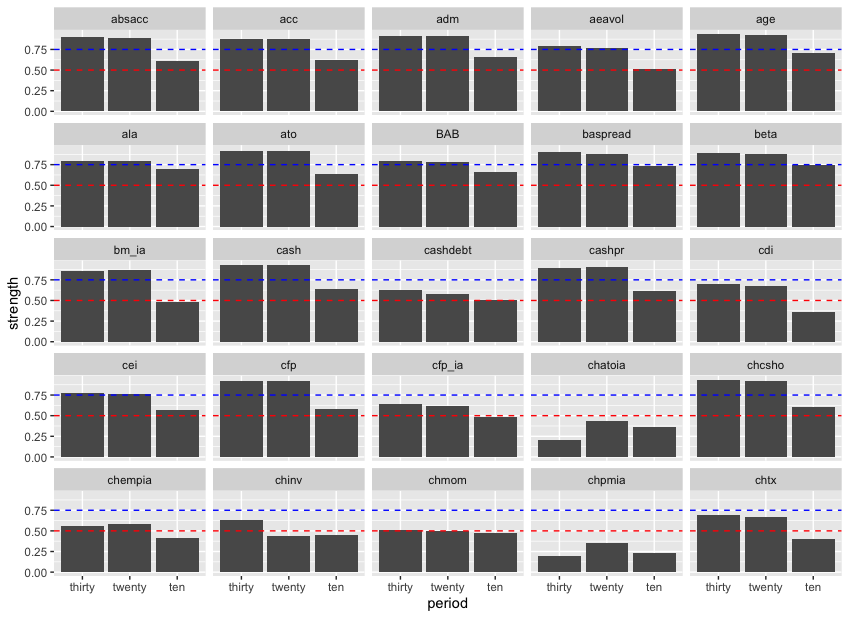
\includegraphics[scale = 0.7]{strength_comparison_I}
			\begin{minipage}{\textwidth}
	{\footnotesize {\bf Notes:} The figure compare the strength of every factor's strength in different data set. The x-axis indicates the data set: thirty is thirty years data set (January 1987 to December 2017), twenty is twenty year data set (January 1997 to December 2017), and ten is ten year data set (January 2007 to December 2017). The red dash line draws from the 0,5 as the 0.5 threshold for weak and strong factor.}
			\end{minipage}
\end{figure}
\end{landscape}



\begin{landscape}
	\begin{figure}[ht]
		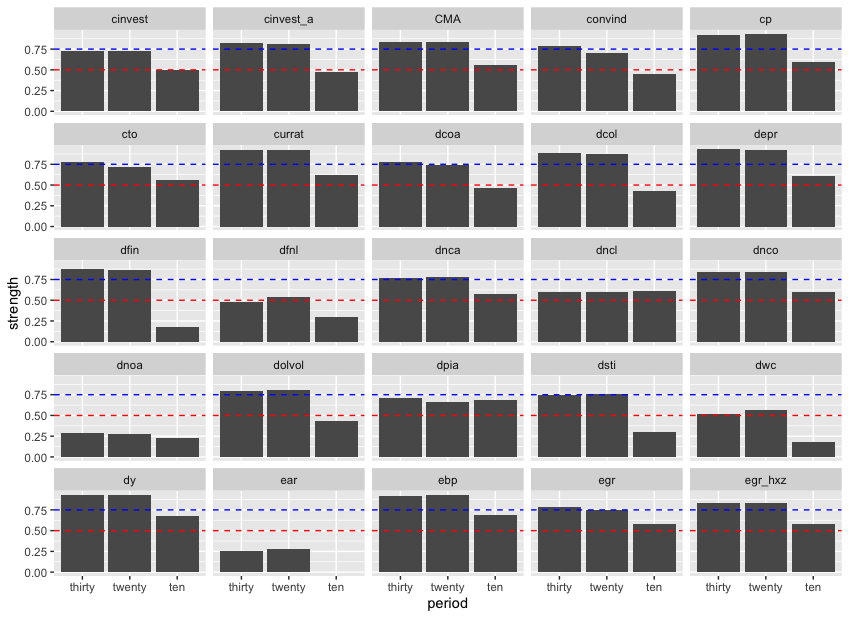
\includegraphics[scale = 0.7]{strength_comparison_II}
		\centering
	\end{figure}
\end{landscape}

\begin{landscape}
	\begin{figure}[ht]
		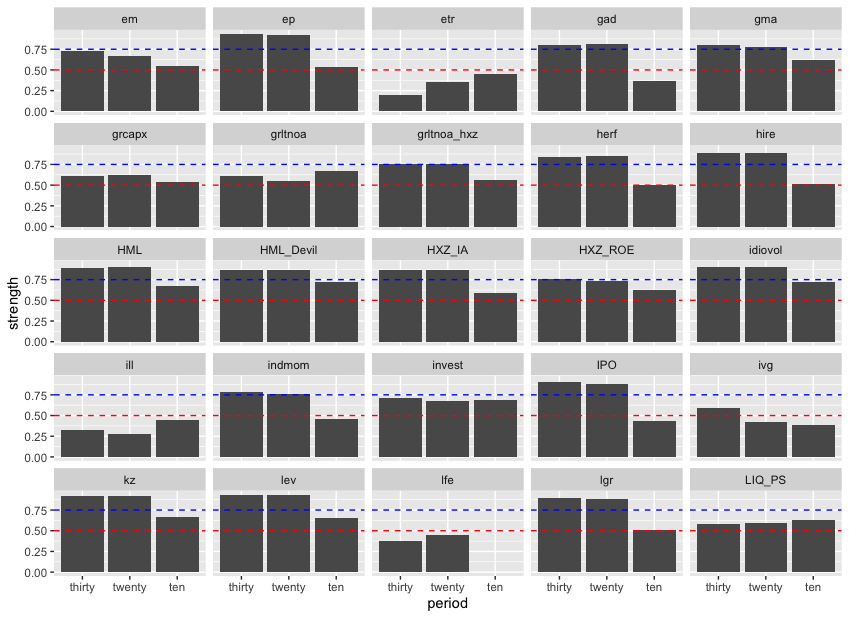
\includegraphics[scale = 0.7]{strength_comparison_III}
		\centering
	\end{figure}
\end{landscape}

\begin{landscape}
	\begin{figure}[ht]
		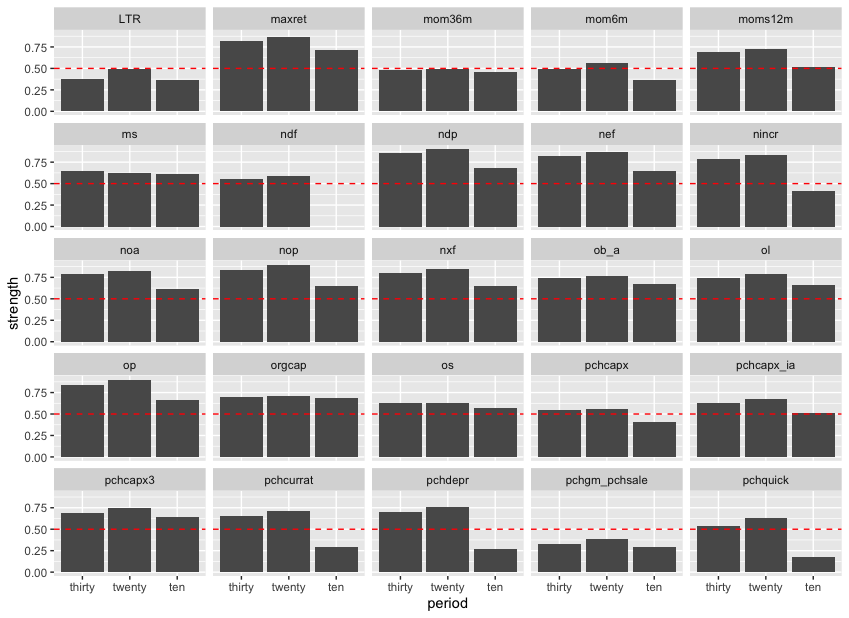
\includegraphics[scale = 0.7]{strength_comparison_IV}
		\centering
	\end{figure}
\end{landscape}

\begin{landscape}
	\begin{figure}[ht]
		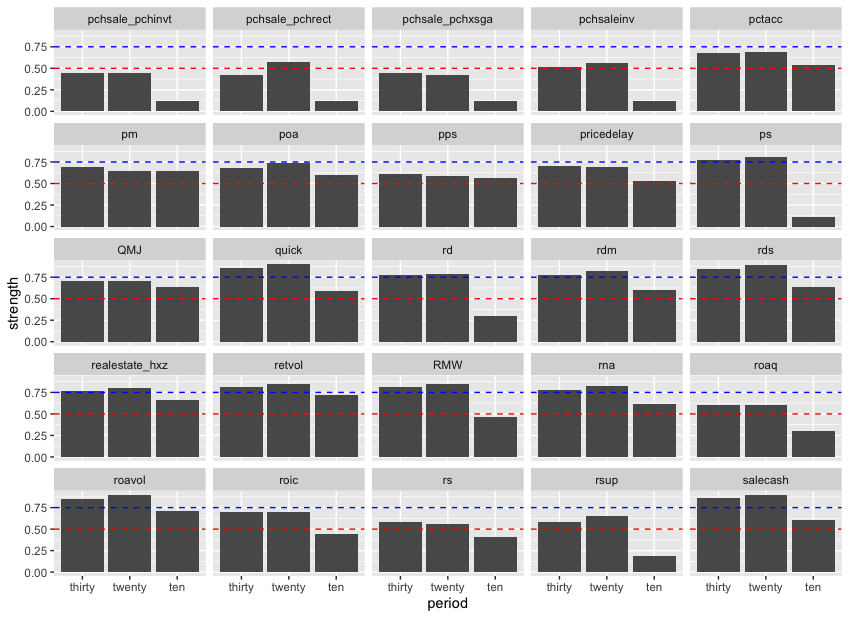
\includegraphics[scale = 0.7]{strength_comparison_V}
		\centering
	\end{figure}
\end{landscape}

\begin{landscape}
	\begin{figure}[ht]
		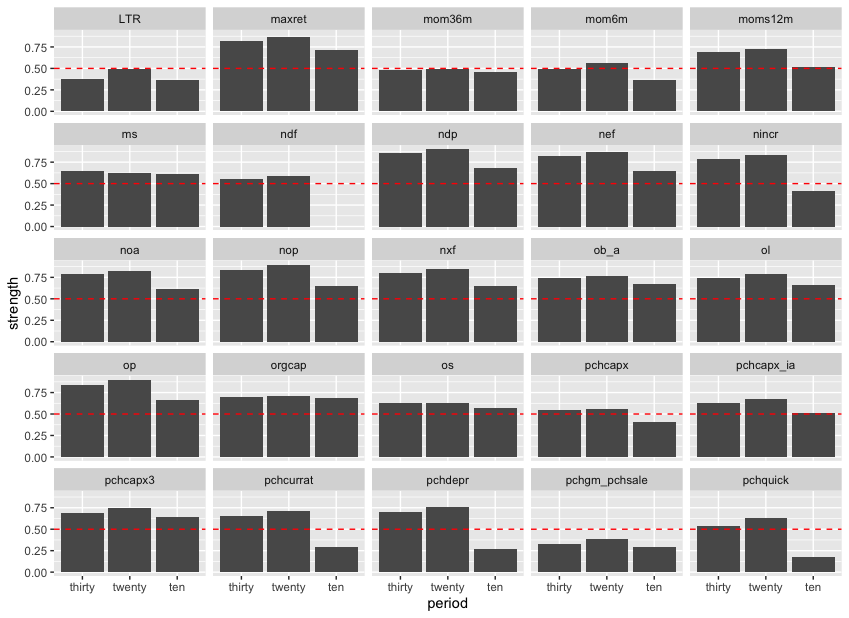
\includegraphics[scale = 0.7]{strength_comparison_IV}
		\centering
	\end{figure}
\end{landscape}

\begin{landscape}
	\begin{figure}[ht]
			\caption{The scatter Plot for three period}\label{figure:scatter}
		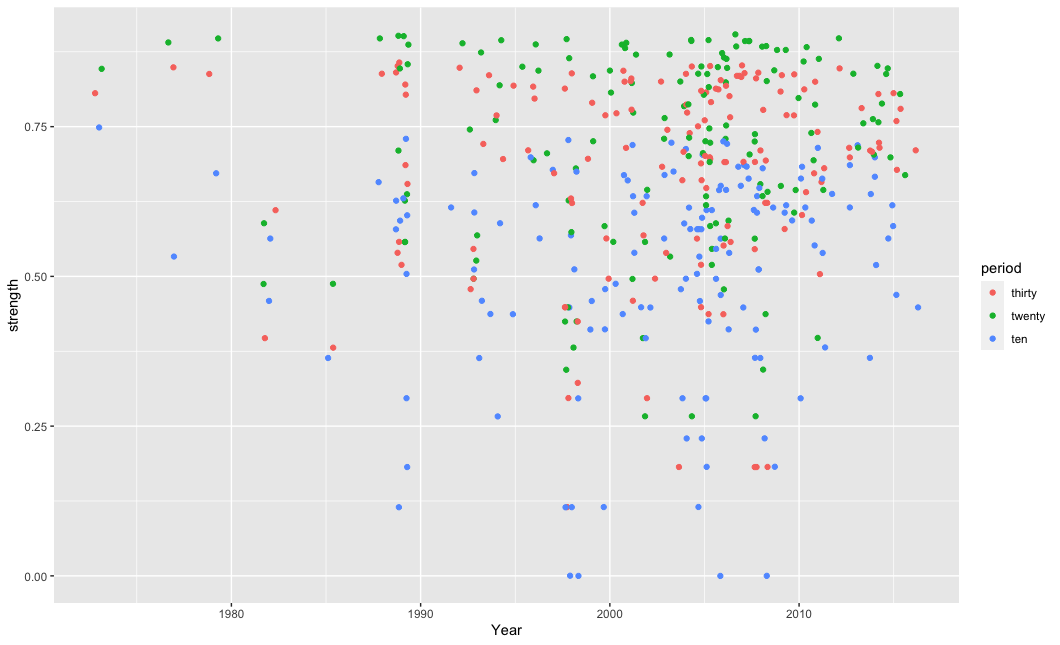
\includegraphics[width=\columnwidth]{scatter}
		\centering
					\begin{minipage}{\textwidth}
			{\footnotesize {\bf Notes:} This scatter plot illustrates the relationship between the factor strength and the factor's publish year. The x-axis represent the year, and the y-axis represent the factor strength. For each factor, we estimate it's strength base on three different data sets, and we use different colour to indicates the three different data set.}
		\end{minipage}
	\end{figure}
\end{landscape}


%\end{document}


%		\end{document}
%\subsection{Elastic Net}

Elastic net  is variable selection model that can be used for factor selection, introduced by \citeA{Zou2005}. Applying elastic net method to estimate the factor loading $\beta_{ij}$ requires:
	\[   \hat{\beta}_{ij}  = \argmin_{\beta_{ij}}\{\sum_{i = 1}^{n}[(r_{it} - r_{ft}) - \beta_{ij }f_{jt}]^2 + \lambda_2\sum_{i = 1}^{n}\beta_{ij}^2  + \lambda_1\sum_{i = 1}^{n}|\beta_{ij}|  \label{ENcriterion} \tag{4}   \}    \]
	
	
	
Because the Lasso regression only contains $L_1$ penalty term $\sum_{i = 1}^{n} |\beta_{ij}|$, it will shows no preference when selecting variables when they are highly correlated.
So when Lasso regression will either randomly choose factors from highly correlated candidates, or eliminate them together as a whole.  
Elastic Net, however, by containing $L_2$ penalty term $\sum_{i=1}^{n}\beta_{ij}^2$, solves this problem. 
The $L_2$ penalty term tend to shrink the potential parameters when they does not provide enough explanatory power, but it will not remove redundant factors.
Therefore, the elastic net method will shrink those parameters associated with the correlated factors and keep them, or drop them if they are redundant at pricing risk. 
	
%\documentclass[12pt]{article}
%\usepackage{amsmath}
%\usepackage{mathptmx}
%\usepackage{setspace}
%\usepackage{amssymb}
%\usepackage{float}
%\usepackage{graphicx}
%\usepackage{booktabs}
%\usepackage{subfigure}
%\usepackage[margin=2.5cm]{geometry}
%\usepackage[title]{appendix}
%\usepackage{bm}
%\usepackage{tcolorbox}
%\usepackage{apacite}
%\onehalfspacing
%\usepackage{lineno}
%\linenumbers
%\usepackage{diagbox}

%\DeclareMathOperator*{\argmin}{arg\,min}
%\newtheorem{experiment}{Experiment}



%\usepackage{fontspec}
%\setmainfont{Times New Roman}
%\addtolength{\jot}{0.5em}
%\linespread{1.5}

%\begin{document}
	\section{Empirical Application}\label{Empirical}
	
Researchers and practitioners have been using the CAPM model \cite{Sharpe1964, Lintner1965, Black1972} and its multi-factor extension (For example, the three-factor model by \citeA{Fama1992}) when they are trying to capture the uncertainty of asset's return.
The surging of new factors \cite{Harvey2019} provides numerous option to construct the CAPM model, but it also requires users to pick the factors wisely.
In this section, we will use two different methods to identify appropriate factors from a group of 146 candidates.
First, we utilise the method introduced in section \ref{strength} to estimates the strength of each factor from the factor group.
Then, we use the strength as a criterion to select factors including in the CAPM model.
In the second part of this section, we apply the elastic net method, ask the algorithm to pick factors for us.
We will compare the factors selected by those two approaches, expected a consistent selection outcome.
Through the empirical application, we also found that under certain conditions, we will obtain a generous CAPM model with too many factors, when using factor strength as the criterion.
Therefore, additionally, we apply the elastic net method to further shrinkage down factor selection.
	\subsection{Data}\label{data}
	
In the empirical application part, we use the monthly returns on U.S. securities as the assets.
The companies are selected from Standard Poor (S\&P) 500 index component companies.\footnote{The companies return data was obtained from the Global Finance Data: http://www.globalfinancialdata.com/,\\ Osiris: https://www.bvdinfo.com/en-gb/our-products/data/international/osiris, \\and Yahoo Finance: https://finance.yahoo.com/.}
We prepared three data sets for different time spans: 10 years (January 2008 to December 2017, T = 120), 20 years (January 1998 to December 2017, T  = 240), and 30 years (January 1989 to December 2017, T = 360).
The initial data set contains 505 companies, but because of the components companies of the index are constantly changing, bankrupt companies will be moved out, and new companies will be added in.
Also, some companies do not have enough observations.
Therefore, for each of the datasets, the number of companies (n) is different, the dimensions of the data set are showing in the table (\ref{Data_set}) below.

\begin{table}[h]
		\caption{Data Set Dimensions}
			\label{Data_set}
	\begin{tabular}{c|ccc}
		\hline
		& Time Span                    & Number of Companies (n) & Observations Amount (T) \\ \hline
		10 Years & January 2008 - December 2017 & 419                  & 120                     \\
		20 Years & January 1998 - December 2017 & 342                  & 240                     \\
		30 Years & January 1988 - December 2017 & 242                  & 360                     \\ \hline
	\end{tabular}
\end{table}
For the risk-free rate, we use the one-month U.S. treasury bill return.\footnote{ The risk free rate was from the Kenneth R. French website: http://mba.tuck.dartmouth.edu/pages/faculty/ken.french/}
For company i, we calculate the companies return at month t ($r_{it}$) using the following formula:
\begin{align*}
r_{it} = \frac{p_{i t} - p_{i t-1}}{p_{i t-1}}\times 100
\end{align*}
and calculate the excess return $x_{it} = r_{it} - r_{ft}$.
Here the $p_{it}$ and $p_{i t-1}$ are the company's close stock price on the first trading day of month t and t-1.
The price is adjusted for the dividends and splits.\footnote{The data is adjusted base on the Central for Research in Security Price (CRSP) method.}

Concerning the factors, we use 145 different risk factors from \citeA{Feng2020}.
The factor set also includes the market factor, represented by the difference between the average market return and risk-free return.
The average market return is a weighted average return of all stocks in the U.S. market, incorporated by CSRP.
Each factor contains observations from January 1988 to December 2017.

\subsection{Factor Strength Analysis}

\subsubsection{Regression model setting}
For the first part of the empirical application, we estimate the factor strength using the method discussed in section \ref{strength}.
More precisely, we set the regression models based on section \ref{strength_multi_estimation}.
\begin{align*}
  x_{it} &= a_i + \beta_{im}(r_{mt} - r_{ft}) + v_{it} \\
 x_{it} &= a_i + \beta_{im}(r_{mt} - r_{ft}) + \beta_{ij}f_{jt} + v_{it} 
\end{align*}

Here $x_{it}$ is the excess return of asset i at time t, which is pre-defined in section \ref{data}.
$r_{mt} - r_{ft}$ represents the market factor, calculated by the difference between average market return and risk-free return at the same time t.
$f_{jt}$ is the value of $j^{th}$ risk factor  at time t. 
Here $j = 1, 2, 3,\cdots 145$ . 
$\beta_{mt}$ and $\beta_{ij}$ are the factor loadings for market factor and risk factor, respectively.

We use two different regressions in the purpose of estimating the strength under the single factor setting and the two factors setting.
However, due to the potential correlations among factors, we will only focus the market factor strength when using the first single factor regression.


	\subsubsection{Factor Strength Findings}
The complete set of results of factor strength estimation is presented in the appendix \ref{strength_table} and \ref{strength_figures}.
We estimated the factors' strength using three different data sets discussed in the \ref{data}, and rank those strength from strong to weak, alongside the market factor strength, in the table (\ref{table:three_ranked_compare}).

We first look at the market factor strength under the single-factor CAPM setting. (see table \ref{table:market})

\begin{table}[]
	\centering
			\caption{Market factor strength estimation} \label{table:market}
	\begin{tabular}{l|ccc}
		\hline
\hline
                                                                                                  & Ten Year Data & Twenty Year Data & Thirty Year Data \\ \hline
\begin{tabular}[c]{@{}l@{}}Market Factor Strength\\ (Single Factor Setting)\end{tabular}          & 0.988         & 0.990            & 0.995            \\
\begin{tabular}[c]{@{}l@{}}Average Market Factor Strength\\ (Double Factors Setting)\end{tabular} & 0.987         & 0.991            & 0.996            \\    \hline \hline
	\end{tabular}
\end{table}
As we expected, the estimated strength of market factor under all three scenarios shows consistently strong results.
All three market factor strengths are close to unity, which indicates that the market factor can generate significant factor loading almost all time for every asset.
Although the value is close to one, we still notice that the strength will increase slightly with the time span extended.
This might indicate that for the security returns, from the long run, it will more closely mimic the behaviours of the market than the short run. 
%=============================%Newly Added%=================================%
Then, we turn to the double factor CAPM setting.
Under the double factor setting, we estimates every companies' stock return using market facto plus another risk factors.
Therefore we will obtain the market factor strength for each single risk factors.
So, we calculate the average market factor here:
\[ \bar{\alpha}_{m} = \frac{1}{145}\sum_{i = 1}^{145}\alpha_{im}   \]
$\alpha_{im}$ is the estimated market factor strength for the $i^{th}$ risk factor setting.
Table\ref{table:market} shows that the estimated strength is consistent with the single factor settings.
All three data sets provides extremely strong results, strengths are close to one.
Overall, the market factor results indicates that the market factor can generate significant loadings for almost every companies' return at any time.
Such conclusion fits with the financial theory states that individual stocks will in general move with the market.
%=============================================================================%
When looking at other factors,  the ten-year data set in general provides a significantly weaker result, compares with the other two data sets results.
Except for the market factor, no other factors from the ten-years result show strength above 0.8.
The strongest factor besides the market factor is the beta factor which has strength around 0.75.
In contrast, the strongest risk factor (factor other than market factor) in the twenty-year data set is the ndp (net debt-to-price), which has strength 0.937.
In the thirty-year scenario, the salecash (sales to cash) is the strongest with strength 0.948.

\begin{table}[hbt!]
	\caption{Proportion of Strength (Excluded Market Factor) }\label{table:proportion}
	\begin{tabular}{lccc}
		\hline
		\hline
		Strength Level & \multicolumn{1}{l}{10 Year Data Proportion} & \multicolumn{1}{l}{20 Year Data Proportion} & \multicolumn{1}{l}{30 Year Data Proportion} \\ \hline
		{[}0.9, 1{]}   & 0\%                                         & 21.4\%                                      & 23.4\%                                         \\
		{[}0.85, 0.9)  & 0\%                                         & 17.9\%                                      & 17.9\%                                      \\
		{[}0.8, 0.85)  & 0\%                                         & 7.59\%                                      & 6.21\%                                      \\
		{[}0.75, 0.8)  & 0\%                                         & 11.7\%                                      & 17.9\%                                      \\
		{[}0.7, 0.75)  & 7.59\%                                      & 8.28\%                                      & 7.59\%                                      \\
		{[}0.65, 07)   & 15.9\%                                      & 8.28\%                                      & 2.76\%                                      \\
		{[}0.6, 0.65)  & 17.9\%                                      & 5.52\%                                      & 8.97\%                                      \\
		{[}0.55, 0.6)  & 13.1\%                                      & 6.21\%                                      & 2.76\%                                      \\
		{[}0.5, 0.55)  & 8.97\%                                      & 4.83\%                                      & 4.14\%                                      \\
		{[}0, 0.5)     & 36.6\%                                      & 8.28\%                                      & 8.28\%                                      \\ \hline\hline
	\end{tabular}
\end{table}

When comparing the proportion of factors with strengths falling in different intervals between 0 and 1 (see table (\ref{table:proportion})), we can find that when using 0.8 as a threshold, there are over forty-five per cent factors in the twenty-year and thirty-year result exceeds this threshold.
In ten year results, the number is zero.
We also find that nearly 40\% of factors from the ten-year dataset show strength less than 0.5, which is almost four times higher than the twenty and thirty years proportion.

When look at the ranking, we found that there are three factors: ndq (Net debt-to-price ), salecash (sales to cash), and quick (quick ratio) who are ranking top three in both twenty year data set result and thirty year data set result.
We would expect when applying the elastic net method with the twenty-year and thirty-year data set, those three factors with the market factors would be selected.

Another interesting finding is that the roavol (Earnings volatility, 10th of ten-year result, 7th of twenty-year result, 5th of thirty-year result ), age (Years since first Compustat coverage, 11th of ten-year result, 9th of twenty-year result, 4th of thirty-year result), and ndp (net debt-to-price, 14th of ten-year result, 1st of twenty-year result, 2nd of thirty-year result).
This might indicates a persistent risk pricing ability of these three factors exist, even with the changes of the data set's dimensions.

\begin{table}[]
	\centering
	\caption{Selected Risk Factor with Strength: top 15 factors from each data set and three well know factors.}
	\begin{tabular}{llc|llc|llc}
		\hline
		\multicolumn{3}{c|}{Ten Year} & \multicolumn{3}{c|}{Twenty Yera} & \multicolumn{3}{c}{Thirty Year} \\ \hline
		Rank & Factor     & Strength & Rank   & Factor     & Strength   & Rank   & Factor     & Strength   \\ \hline
%	 	 & Market & 0.988 & &Market & 0.990 & &Market & 0.995 \\
		1   & beta               & 0.749    & 1      & ndp           & 0.937      & 1      & salecash  & 0.948\\
		2   & baspread       & 0.730    & 2      & quick        & 0.934      & 2      & ndp          & 0.941\\
		3   & turn               & 0.728    & 3      & salecash   & 0.933      & 3      & quick      & 0.940\\
		4   & zerotrade      & 0.725    & 4      & lev            & 0.931      & 4      & age         & 0.940\\
		5   & idiovol           & 0.723    & 5      & cash         & 0.931      & 5      & roavol    & 0.938\\
		6   & retvol            & 0.721    & 6      & dy             & 0.929      & 6      & ep           & 0.937\\
		7   & std\_turn      & 0.719    & 7      & roavol      & 0.929      & 7      & depr       & 0.935\\
		8   & HML\_Devil & 0.719    & 8      & zs              & 0.927      & 8      & cash       & 0.934\\
		9   & maret           & 0.715    & 9        & age          & 0.927      & 9      & rds         & 0.931\\
		10 & roavol          & 0.713    & 10     & cp             & 0.926      & 10    & dy          & 0.927 \\
		11 & age               & 0.703    &11      & ebp           & 0.926      & 11     & currat   & 0.927 \\ 
		12 & sp                 & 0.699    &12      & op            & 0.925      &12       & chcsho  & 0.927 \\ 
		13 & ala                & 0.699    &13      & cfp          & 0.924       &13      & lev         & 0.926 \\ 
		14 & ndp              & 0.686    &14      & nop          & 0.924       &14     & stdacc     & 0.926 \\ 
		15 & orgcap         & 0.686    &15      & ep            & 0.923       &15     & cfp          & 0.925 \\ 
		20 & UMD            & 0.678    & 29     & HML        & 0.905      & 39     & HML       & 0.894 \\
		24 & HML            & 0.672    & 76     & SMB        & 0.770      & 68     & SMB        & 0.804 \\
		87 & SMB            & 0.512    & 89     & UMD        & 0.733      & 96     & UMD       & 0.745 \\ 
		\hline
	\end{tabular}
\end{table}
%But it worth notice that the market factor is consistently strong.
%The strength of market factor is close to unity all the time in the twenty year result, but decrease gradually when the t is growing %and n is decreasing.
%However, we also find that the market factor strength will decrease with the increase of observation and decrease of units.
%For instance, the market factor in the twenty year results, in general, it decrease from 0.98 to around 0.96, and it decreased %further to 0.9 in the thirty year estimation result.
%But not matter in which data set, the market factor is always the strongest factor.

%\begin{table}[]
%	\centering
%		\caption{Fama and French value and size factor, with Momentum Factor strength}
%	\begin{tabular}{l|ccc}
%		\hline
%		\hline
%		Factor & Ten Year Estimation & Twenty Year Estimation & Thirty Year Estimation \\ \hline
%				SMB (Size)    & 0.512               & 0.745                  & 0.721                  \\
%		HML (Value)    & 0.672               & 0.873                  & 0.811                  \\
%		UMD  (Momentum)  & 0.678               & 0.703                  & 0.672                  \\ \hline \hline
%	\end{tabular}
%\end{table}

We also focus on some well-known factors, namely the Fama-French size factor (Small Minus Big SMB), Fama-French Value factor (High Minus Low: HML) \cite{Fama1992} and the Momentum factor (UMD) \cite{Carhart1997}.
It is surprising that none of these three factors enters the top fifteen list for each data sets.
Except for the HML factor from the twenty and thirty-year data set has strength closely around 0.9, none of the other factors in any data set shows strength higher than 0.85.
%The value factor SMB from the ten year data set only has strength 0.512, ranked no.87.
When using the ten-year data, both UMD and HML has strength around 0.67, and the SMB only has strength 0.512.
Results from the twenty-year data set show that HML has strength 0.905, for SMB and UMD the strength are 0.770 and 0.733 respectively.
Comparing with the twenty-year results, the thirty-year estimated strength change slightly, HML decreases to 0.894, SMB is 0.804 and UMD has strength 0.745.
Therefore, when using the strength as a criterion, we may only select the value factor to incorporate in the CAPM model when having twenty and thirty-year data.

In general, we found that the twenty-year and thirty-year data sets provides similar estimated strength, while, in contrast, the estimated strengths from ten-year data set are significantly weaker.
Therefore, as a second step, in order to see how factor strengths evolve through the time, we decompose the thirty yea-data set into three small subsample.
For each subsamples, it contains 242 companies (n = 242). 
And for each company, we obtained 120 observations (t = 120). 
The results are present in the table (\ref{table:thirty_decompose}) and figure (\ref{figure:thirty_decompose}).

In general, we can conclude that about 80\% factors, their strength gradually increased from the first decade (January 1988 to December 1997) to the second decade (January 1998 to December 2007), and then decreased in the third decade (January 2008 to December 2017).
This pattern can also be seen in the figure (\ref{figure:thirty_decompose}).
The drop of factor strength in the third decades can be reconciled with the ten-year data results shows a significantly weaker strength than the results from twenty and thirty years data set.

%has been regards as the main reasons why the ten-years data results shows a significantly weaker results than the twenty and thirty years data set.


%The strength has been dragged down by the data from 2007 to 2017.
%One possible explanation is that the Great Financial Crisis happened during the 2007 to 2008 has distorted the risk pricing mechanism of some factors.

%Also, from the simulation results (see appendix \ref{simulationtable}), we find that when the n < t, in other words, when the units is less than the observation, the overall bias will be negative.
%This indicates that the strength from the thirty-year data is underestimated.
%After taking this correction into consideration, we may have a more close results between the twenty and thirty years dataset estimations.
%For some factors does not follow this rule, we find that they usually have very weak strength in all three periods, for instance the std\_dolvol (volume of liquidity) factor, we can see that in all three periods, the strength has never excess the 0.5 threshold.

%\subsubsection{Conclusion and Explanation}
Overall from the factor strength prospect, we would expect that for different time periods, we will have different candidate factors for the CAPM model.
For the ten-year data set, we would expect that only the market factor be useful, and therefore the elastic net method applied latter may only select the market factor.
If we use the twenty and thirty-year data, we will have a longer list for potential factors, 62 factors from the twenty-year estimation and 45 from the thirty years has strength greater than 0.8.
Hence, we would expect the elastic net to select a less parsimonious model. 

In terms of the findings we have above, there are several potential explanations.
First, if we consider the structure of our data set, we will find that the longer the time span, the fewer companies are included.
This is because the S\&P index will adjust the component, remove companies with inadequate behaviours, and add in new companies to reflect the market situation.
Hence, those 242 companies in the thirty-year data set can be viewed as survivals after a series of financial and economic crisis.
We would expect those companies will have above average performances, such as better profitability and administration, compared with other companies. 

%{\bf Notes: (But for how will those merits influence the factor's risk pricing ability is unclear for now)}

Another possible explanation the happening of a series of political and financial unease from the time of late 20 century to 2008.
Crisis like the Russia financial crisis in 1998, the bankruptcy of Long Term Capital Management (LTCM) in 2000, the dot com bubble crisis in early 21st century and the Global Financial Crisis (GFC) in 2008 creates market disturbances.
Such disturbances, however, provides extra correlations among factors.
The extra correlations enable some factors provides additional pricing power risk.
But we should also notice that the financial market has been disturbed by those crises so, therefore, some mechanism may no longer working properly during that period.
Which means that those crises will also have negative influences on factor when they are capturing the risk-return relationship.

We also need to notice that for some factors, their strength will decrease with time.
For instance, the gma (gross profitability) factor and dwc (change in net non-cash working capital) factor (see figure \ref{figure:thirty_decompose}) has consecutive strength decrease from the 1987-1997 period to 2007-2017 period.
And for most of the factors, their strength will decrease significantly from the 1997-2007 period to 2007-2017 period.
Therefore, disqualify some factors as the candidate of the CAPM model when using recent year data is inevitable.




%Beside, from the simulation results (see appendix \ref{simulationtable}), we find that when we have a unbalanced panel (when n < t, the unit is smaller than the observation), we will have negative bias results.
%This indicates that the strength is underestimated in that scenario.
%Therefore, we could inference that the factor strength will be stronger than what we estimated if we use the thirty-year data.
%After taking this correction into consideration, we may have a more closer results between the twenty and thirty years estimation.

%From the estimation, we see the factor strength will change through time.
%And from the factor selection prospect, we would expect to have selecting different factors when using different dataset, there is no unanimity factors with regard of risk pricing.
%The decomposition of thirty years data shows that most factors' strength increases from the first decade (January 1988 - December 1997) to the second decade (January 1998 to December 2007), and then drops in the third decade (January 2008 to December 2017).
%But from the simulation result (see section \ref{MC} and appendix \ref{simulationtable}), we can see that when the observation amount is larger than the unit amount, i.e. when the t > n, we have negative bias, which indicates that the estimated strength $\hat{\alpha}$ is smaller than the true strength $\alpha$.
%In the thirty year data set, we have t = 360, and n = 242.
%Therefore, we can reasonable assume that the factor strength is under estimates.
%Consider such correction, the true strength of factor using data from the thirty year data to estimates may have similar strength as using twenty year data.

%\begin{table}[]
%	\centering
%	\caption{RMSE between different data set estimation result}\label{table:RMSE_strength}
%	\begin{tabular}{rl|r}
	%	\hline
%		\hline
%		& Pair           & Difference \\ \hline
%		1 & Ten : Twenty    & 0.254 \\
%		2 & Ten : Thirty    & 0.220 \\
%		3 & Twenty : Thirty & 0.06  \\ \hline \hline
%	\end{tabular}
%\end{table}

%We also use the formula:
%\[ Differnce  = \sqrt{\sum_{i = 1}^{145}(\widehat{\alpha_{xi}} - \widehat{\alpha_{yi}})^2}  \]
%to calculates the Root Mean Square Difference between any two different strength results (see table(\ref{table:RMSE_strength})).
%Here the $\widehat{\alpha_{xi}}$ and $\widehat{\alpha_{yi}}$ each represents the estimates factor strength of $i^{th}$ factor from different data sets. 
%The difference between twenty and thirty year data sets results is significantly smaller than the differences between ten-twenty and ten-thirty.




%\newpage
%\bibliographystyle{apacite}
%\bibliography{thesis.bib}
%\end{document}
\section{Elastic Net and Application}\label{Empirical:Elastic_net}
%\subsection{Introduction of empirical method and data}
As we introduced before, the surging number of risk factors post question of which factors can independently provides unique information to explain the risk-return relationship. \cite{Cochrane2011}.
In this section, we employed the Elastic net algorithm to discuss this problem.
We also compare the Elastic net results with the Lasso regression.
We first briefly introduce the core idea of elastic net method, explained what's the different between Elastic net and other factor selection methods.
Then, we provides a full discussion of how to select the tuning parameter with regard of the Elastic net method when using r package \textit{glmnet} to imply the elastic net.
Finally, we compare and discuss the findings from both Elastic net and Lasso.


\subsection{Brief introduction of Elastic Net} \label{Elastic_Net}

Elastic net,introduced by \citeA{Zou2005},  is a penalised linear regression method which developed from the Lasso regression \cite{Tibshirani1996} and ridge regression.
To illustrate the application of elastic net method in our research, first recall the multi-factor model (\ref{multi_factor_model}) we discussed in section \ref{strength_multi_estimation}.
When applying the OLS on estimating the factor loading $\bm{\beta_{i}}$, we targeting minimise the Residual Sum of Squares (RSS):
\[  \bm{\hat{\beta}}_i =   \argmin\{  (x_{it} - \hat{a}_{iT} - \bm{\hat{\beta}}_i^{\prime}\bm{f}_t )^2 \}    \]
In the method of elastic net, base on the RSS minimisation, we impose two extra penalty terms on the estimated loadings:
\[   \bm{\hat{\beta}_{i}}  = \argmin_{\beta_{ij}}\{ (x_{it} - \hat{a}_{iT} - \bm{\hat{\beta}}_{i} ^{\prime}\bm{f}_{t})^2 + \lambda_2\sum_{j = 1}^k\hat{\beta}_{ij}^2  + \lambda_1\sum_{j=1}^k|\hat{\beta}_{ij}|  \label{ENcriterion} \tag{11}   \}    \]
Here, the estimated $\bm{\beta}_i$ value is subject to two penalty terms: the $L^1$ norm $\lambda_1\sum_{j=1}^k|\hat{\beta}_{ij}|$ and the $L^2$ norm: $\lambda_2\sum_{j = 1}^k\hat{\beta}_{ij}^2$.
The adoption of combing $L^1$ and $L^2$ norm allowing as to fix the problem from both ridge regression (only contains the $L^1$ norm), and the Lasso regression (only contains the $L^2$ norm).
In the empirical application, the estimation of the of Elastic net usually use the following form:
\begin{align*}
	\bm{\hat{\beta}}_{i} &= \argmin\{ \frac{1}{2N} (x_{it}-\hat{a}_{iT} - \bm{\hat{\beta}_{i}^{\prime}}\bm{f}_t ^2 ) +\phi P_{\theta}(\bm{\beta}_i)  \}\\
	P_{\theta}(\bm{\beta}_i) &=\sum_{j=1}^k [ (1-\theta)\beta_{ij}^2 + \theta |\beta_{ij}|]
\end{align*}
Here we call the $P_{\theta}(\cdot)$ as the elastic net penalty \cite{Friedman2010}.
$\theta$ here act as turning parameter to determine in what extent the Elastic net will behave like a ridge regression or like a Lasso regression.
When set $\theta = 1$, we have $P_{\theta}(\bm{\beta}_i) =\sum_{j=1}^k  |\beta_{ij}|$ which is identical to the $L^2$ norm, therefore we have the Elastic net collapse to the Lasso regression.
Similarly, when setting $\theta = 0$, we have the Elastic net collapse to the ridge regression, and when $\theta = 0.5$, the Elastic net is behave like the combination of ridge and Lasso.
The other tuning parameter $\phi$ decides how strong the penalty terms is.
If $\phi = 0$ the elastic net will become the OLS estimation.

In this study, we use the data introduced in section \ref{data}, and the estimated factor strength from the section \ref{Empirical}.
More specifically, we allocates the 145 risk factors into six subgroups base on there thirty-year data set estimated strength.
For each subgroups, we randomly selected ten factors, and we want to investigates how will the elastic net algorithm, alongside with ridge and Lasso regression, will select the factors for risk pricing.
Noticed here, in order to simplify the application of the elastic net, instead of using the excess return of stock directly, we first run a OLS regression between the market factor and the excess return of each companies.
And then, we collect the residuals of the OLS estimation, and use those residuals as the $x_{it}$ in the elastic net model.
This is because, both the theory and the findings from the previous section suggest that the market factor will be included into the CAPM model for every assets.

Now, the main challenge of applying the elastic net algorithm is to select the appropriate tuning parameters $\theta$ and $\phi$, and we will discuss the choices of tuning parameter in the next section.

%\subsection{Empirical procedure of Elastic Net}
%In this subsection we will brief introduce the empirical investigation stpes
	\subsection{Brief Properties of Risk Factors}
We start with a brief discussion about the risk factors before applying the elastic net method.
The risk factors data set contains 145 risk factors at the monthly frequency fro the period from July 1976 to December 2007.\footnote{For how those factors are constructed, please view \citeA{Feng2020}}
To exam the stationarity of the risk factor series, we employed Augmented Dick-fuller (ADF) test \cite{Dickey1979},  Phillips-Perron (PP) test \cite{Phillips1988}, and the Kwiatkowski-Phillips-Schmidt-Shin (KPSS) test \cite{Kwiatkowski1992}.
In general, ADF test and PP test provides same conclusions that all 145 risk factor series does not contains unit root.
The KPSS test, however, disagree with the ADF and PP test.
If we take 0.05 as the threshold of p-value, the KPSS test concludes that there are six factors contain unit root in their process.


\subsection{Tuning Parameter} \label{EN:parameter_tuning }
In this empirical application, we use the R package \textit{glmnet} \cite{Friedman2010, Simon2011}.

As discussed before, the estimation of Elastic net in our application is up on two tuning parameters $\theta$ and $\phi$.
The \textit{glmnet} package provides function to select the $\phi$ automatically. 
This selection is base on the minimisation of Mean Squared Error (MSE), using cross validation.
However, the package does not provides aid on determining which value of $\theta$ parameter is optimal.
Therefore, we adopt the following strategy to select our tuning parameters $\phi$  and $\theta$:
\begin{enumerate}
\item Prepare a sequence of $\theta$ values, from 0: ridge regression, to 1: Lasso regression with step of 0.01
\item Randomly assign 90\% of the data set as training set and the rest 10\% as test set. 
\item For each of the $\theta$ value, we fit the corresponding Elastic net model using the training set, with function picked $\phi$ values.
\item Base on the $\theta$ and $\phi$ values select, we produce the predicted values using the test data, and calculates the MSE between the true values and predicted values.
\item We select the $\theta$ which produces the minimal MSE.
\item And the $\phi$ value will be picked up by the package function, base on the principle of minimising MSE.
\end{enumerate}
We repeat the above procedures for 2000 times, and average each $\theta$ values to generate $\bar{\theta}$, as our selected tuning parameter.
Due to the computational burden, when implying the step 2, we will further randomly select 50 companies instead of using all 242 companies returns to estimated the $\theta$.

\begin{table}[]
	\centering
	\caption{Estimated Optimal $\theta$ values for different factor groups}
	\label{table:optimal_theta}
	\begin{tabular}{l|cccc}
		\hline
		\hline
		Factor Group            & (0, 0.5{]}   & (0.5, 0.6{]} & (0.6, 0.7{]} & (0.7, 0.8{]} \\ 
		Selected $\theta$ value & 0.377        & 0.401        & 0.429        & 0.411        \\ \hline
		Factor Group            & (0.8, 0.9{]} & (0.9, 1{]}   & Mix          & Random       \\ 
		Selected $\theta$ value & 0.396        & 0.413        & 0.448        & 0.431        \\ \hline
		\hline
	\end{tabular}
\end{table}
The selected tuning parameter $\theta$ values is shown in the table \ref{table:optimal_theta}.\\
In order to fully investigate the behaviours of parameter tuning, on the basis of the six subgroups, we create tow addition groups.
The Mix group contain five highly strong factor: factor with strength higher than 0.9, and five weak factor: factor with strength lower than 0.5.
The Random group is consist by ten randomly selected factors.
From the table \ref{table:optimal_theta} we can see that the selected $\theta$ value in general increase with the factor strength increase.
For weak factor group, the selected parameter value is 0.377, close to the ridge regression.
While for the strong factor group, the value is 0.413.
The mix factor group has the highest $\theta$ value 0.448, which is close to 0.5 where ridge and Lasso regression each plays half role on the elastic net.

Such pattern of the $\theta$ value, however, does not follow what we expected.
Because the definition of factor strength indicates that factor with strong strength is able to produce more significant loadings, in other words, can explain more assets' risk-return relationship.
Therefore, when using the above procedure to decide tuning parameter, we would expect that for factor groups with lower strength, like groups with strength smaller than 0.5, the selected $\theta$ parameter will be close to one, or larger than other groups' selected $\theta$.
This is because factor with weak strength will only provides limited pricing power, and therefore may be recognised by the algorithm as redundant variables.
When $\theta$ is closer to unity, the elastic net is behave more like a Lasso, which will eliminate variables provides limited explaining power.
In contrast, when the group has stronger strength, the $\theta$ will approach closer to zero, leads the Elastic nets more like Ridge, which will not eliminate any variables, but only reduce the coefficient.
So we would expect the $\theta$ value to increase with the group strength decrease.

We prepared several potential explanation for this result.
First, the MSE is not a ideal criteria for selecting the tuning parameter.
The MSE for all $\theta - \phi$ combinations are very close to each other.
All MSE results shows similar values around 64.
Second, because of the estimation method we used, the market risk has already been absorbed by the market factors.
Then for the strong factor, we would expect that for any single of them, those strong factor can individually explained most of the idiosyncratic risk.
Therefore, when we ask any ten strong factors to determine the risk simultaneously, it is possible that very few of the ten factors can explain most of the risk and therefore the other risk factors will be recognised by the algorithm as redundant.
But if all factors are weak, it is possible that there exist some linear combinations among weak factors provides enough explaining power for the idiosyncratic risk.
Therefore, those weak factors will be reserved by the algorithm, and hence, the parameter $\theta$ will close to zero, indicates a more Ridge like regression.


%However, the empirical findings are not completely accord with what we expect.
%First, MSE does not provides very good indication of selecting $\theta$.
%The MSE values only present very slightly difference among different $\theta-\phi$ combinations.
%And from the prospect of error's value, they are all fairly big: around 64.
%Second, although the $\theta$ values show numerical difference, and it also shows a decreasing pattern with the increasing of factor strength.
%The decreasing magnitude is not as big as we expected.
%Our estimated $\theta$ values for the 0.9 strength group is 0.41, while for the group below 0.5, the corresponding $\theta$ is 0.54. 
%Also, where exist an damp, when the factor has strength in the group of 0.7 to 0.8, the estimated optimal value of $\theta$ decrease to 0.39.



\subsection{Elastic Net Findings}
We applied the elastic net algorithm with tuning parameters determined in the previous section to the thirty-year data set.
The reasons why we use the thirty-year data instead of ten or twenty year is that the Monte Carlo simulation result (see section \ref{MC_findings} and Appendix \ref{simulationtable}) indicates us that the estimation accuracy of factor strength will improve significantly with the increase of time-spam.
Such improvement will not diminish even when the sample size n is small.
Therefore, we use the factor strength result estimated base on the thirty year data set.

We divided the 145 risk factors into six groups base on their factor strength.
We also randomly selected ten factors from  weak factor group (factor with strength less than 0.5), and ten factors from strong factor group (factor with strength above 0.9) to form a mixed factor group.
For each factor groups, we run two regression: the elastic net regression with $\theta$ values presented in the table \ref{table:optimal_theta}, and the Lasso regression with $\theta = 1$.
Instead of running a pooled regression, we run the elastic net and Lasso to each individual companies.
And then we compare for each single stock, how similar the factors selection made by Elastic net and Lasso are agreed with each other.
For every single company, if both Elastic net and Lasso select the same factor (generates factor loading not equals to zero), and disregard the same factor (generate factor loadings equal to zero), then we call that company's stock has exact agreement of factor selection.
We also extend our standard of agreement to 90\% interval, if the Elastic net and Lasso select same factors about 90\% of the total factor amount, we call the stock has a 90\% agreement.
The proportion of agreement is presented in the table\ref{table:proportion_agreement}.

\begin{table}[h]
	\centering
	\caption{Proportion of Lasso Regression and Elastic Net produces same or largely similar results for 145 companies}
	\label{table:proportion_agreement}
	\begin{tabular}{c|ccccccc}
		\hline
		\hline
		\multicolumn{1}{l|}{Factor Group}                                         & \multicolumn{1}{l}{(0,0.5{]}} & \multicolumn{1}{l}{(0.5, 0.6{]}} & \multicolumn{1}{l}{(0.6, 0.7{]}} & \multicolumn{1}{l}{(0.7, 0.8{]}} & \multicolumn{1}{l}{(0.8,0.9{]}} & \multicolumn{1}{l}{(0.9,1{]}} & Mix    \\ \hline
		\begin{tabular}[c]{@{}c@{}}Proportion of Agreement\\ (Exact)\end{tabular} & 68.7\%                        & 55.9\%                           & 42.8\%                           & 20.9\%                           & 17.7\%                          & 13.9\%                        & 34.6\% \\
		\begin{tabular}[c]{@{}c@{}}Proportion of Agreement\\ (90\%)\end{tabular}  & 86.8\%                        & 72.0\%                           & 74.5\%                           & 72.0\%                           & 79.8\%                          & 74.4\%                        & 76.1\% \\ \hline\hline
	\end{tabular}
\end{table}

It is clear that the proportion of agreement, both exact agreed and 90\% agreed, shows a decreasing trend accompany with the factor strength increase.
Nearly 70\% factors selection are identical in the 0 to 0.5 strength group, but this number will decrease to 55\% if the factor strength increase 0.1.
Only 14\% companies has identical factor selection results for for group with strength between 0.9 and 1.
For the mixed strength group, the exact agreed proportion is 34.6\%, ranked between the 0.6 to 0.7 group and 0.7 to 0.8 group.

% expect to see the factor with strong strength will be picked by more companies than factor with weak strength.
%The result in general coincide with our inference: factor with strength less than 0.5 is significantly less selected by the algorithm, for both Lasso and elastic net.
%But we are surprised to see that, when comparing the result within the group, factor selection proportion is not strictly agree with the factor strength.
\begin{table}[h]
	\centering
	\caption{Correlation Coefficient among different factor groups. }
	\label{table:Correlation}
	\begin{tabular}{l|cccccc}
		\hline
		\hline
		Factor Group                                 & (0,0.5{]} & (0.5, 0.6{]} & (0.6, 0.7{]} & (0.7, 0.8{]} & (0.8,0.9{]} & (0.9,1{]} \\ \hline
		\multicolumn{1}{c|}{Correlation Coefficient} & 0.0952    & 0.157        & 0.213        & 0.229        & 0.371       & 0.724   \\
		Factor Amount &12 & 10 &  17 & 37& 35 &34  \\ \hline \hline
	\end{tabular}
\end{table}

We calculate the correlation among factors for each factor groups.
The result is presented in the table \ref{table:Correlation}.
We can clearly see a increasing trend of the correlation coefficient with the increase of factor's strength.
Focusing on the strong factor group, it is clear that a leap exist.
The correlation coefficient doubled from (0.8, 0.9] group to (0.9, 1] group.
This correlation pattern provides a possible explanation of the discord results of Elastic net and Lasso.
When facing variables with high correlation, Lasso will randomly select several variables and discard others.
While Elastic net address this problem with the help of the extra $L^2$ norm in it's loss function.
Therefore, the Elastic net method will select all factors that can bring new information to explain the risk-return relationship even those factors are highly correlated.
On average, Lasso will select about 2.4 less factors than the Elastic net when facing strong factor groups, which contains 34 factors.




	\chapter{Conclusion and Possible Extension}\label{Conclusion}
		\section{Conclusion}
In this thesis, we propose the concept of factor strength and the corresponding estimation method.
We applied the estimation on 145 different risk factors plus the market factor, estimating their strength and use the strength as reference to categorised each factors to reduce the dimension of potential factor group.
On the basis of dimension-reduced factor group, we applied two feature selection methods namely Lasso and Elastic net, trying to eliminate the redundancy of factor groups. 

From the factor strength estimation, we have a consistent estimation result of most of the strong factors.
In general, factor strength will evolve in an upward manner with time increasing.
And the strong factors will keep high strength through times.
But we also notice that the overall factor strength is significantly lower when we use data set contains short time-span, compare with results obtained from using larger data set with more observations.
Also, it worth to notice that some conventionally strong factors, for instance, the size factor, value factor, and the momentum factor do not show particular high strength.

The empirical results of feature selection indicates that both Elastic net method and Lasso regression are both able to correctly and effectively eliminate factors without the ability to generating sufficient factor loadings.
In another word, both Elastic net and Lasso can identify factor with weak strength and disregard those redundant features.
However, since the factors with strong strength are almost all highly correlated, the Elastic net and Lasso fail to make a mutual agreement when facing strong factors.
On average, Elastic net will selects two more factors than Lasso when facing factors with strength above 0.9.
We also noticed that when factors with different are mixed with each other, both lasso and elastic net can effectively pick up factor with strong strength and disregard weak factors.

\section{Possible Extension}

During the empirical exploration, we discovered some possible extension of this paper, and because of the time-limit as well as other restrictions, we could not propose those extensions.
Here, we summarise those potential extensions to provide a starting point for future research.

Firstly, when discussing the factor strength, we ignore the heterogeneity of companies and factors.
Ideally, companies and factors should be categorised based on their nature.
For instance, companies from different industries may react differently to different factors.
Therefore, one possible treatment is to group companies base on their industries types, or categorised factors base on their economical or financial meanings.
Also, \citeA{Harvey2019} suggests that newly propsoed factors are more likely to encounter the multiple=testing problem, and hence they are more likely to be the factors that can not independently provides information to explain risk-return relationship.
So, we could also categorised the factors base on their published time, and to investigates the relationship between factor strength and time.


Secondly, as discussed in the chapter \ref{EN:parameter_tuning },the principle of parameter tuning when applying elastic net is to select the parameter combination that minimise the MSE.
However, the results present in the corresponding chapter indicates that MSE can not distinction different parameter combination significantly enough.
Hence, considering use other criteria may lead to better performance of parameter tuning, and therefore improve the results of the Elastic net application.

Also, some other feature selection methods or dimension reduced techniques can be taken into consideration.
The application of those methods can be used to cross-check with the results of Elastic and Lasso.
Some potential methods including simple stepwise selection method, dantzig selector, and tree-based method like decision tree.







\newpage
\bibliographystyle{apacite}
\bibliography{library.bib}


\newpage
\appendix

%\documentclass[12pt]{article}
%\usepackage{amsmath}
%\usepackage{mathptmx}
%\usepackage{setspace}
%\usepackage{amssymb}
%\usepackage{float}
%\usepackage{graphicx}
%\usepackage{booktabs}
%\usepackage{subfigure}
%\usepackage[margin=2.5cm]{geometry}
%\usepackage[title]{appendix}
%\usepackage{bm}
%\usepackage{tcolorbox}
%\usepackage{apacite}
%\onehalfspacing

%

%\begin{document}

	
	\section{Simulation Result}\label{simulationtable}
\begin{table}[!hbt]
		\caption{Simulation result for single factor setting}\label{table:exp1}
	\centering

	\begin{tabular}{lccccccccc}
		\hline
		\hline
		\multicolumn{1}{l|}{}                   & \multicolumn{9}{c}{Single Factor}                                                               \\ \hline
		\multicolumn{1}{l|}{}                   & \multicolumn{3}{c|}{Bias $\times$ 100}        & \multicolumn{3}{c|}{RMSE $\times$ 100}     & \multicolumn{3}{c}{Size $\times$ 100} \\ \hline
		\multicolumn{10}{c}{$\alpha_1 = 0.7$}                                                                                                                            \\ \hline
		\multicolumn{1}{l|}{n\textbackslash{}T} & 120    & 240    & \multicolumn{1}{c|}{360}    & 120   & 240   & \multicolumn{1}{c|}{360}   & 120         & 240         & 360        \\ \hline
		\multicolumn{1}{l|}{100}                & 0.256  & 0.265  & \multicolumn{1}{c|}{0.227}  & 0.612 & 0.623 & \multicolumn{1}{c|}{0.560} & 7.85        & 7.7         & 5.55       \\
		\multicolumn{1}{l|}{300}                & 0.185  & 0.184  & \multicolumn{1}{c|}{0.184}  & 0.363 & 0.338 & \multicolumn{1}{c|}{0.335} & 8.9         & 4.45        & 4.5        \\
		\multicolumn{1}{l|}{500}                & 0.107  & 0.124  & \multicolumn{1}{c|}{0.109}  & 0.259 & 0.248 & \multicolumn{1}{c|}{0.234} & 6.9         & 2.5         & 1.6        \\ \hline
		\multicolumn{10}{c}{$\alpha_1 = 0.75$}                                                                                                                          \\ \hline
		\multicolumn{1}{c|}{100}                & -0.178 & -0.159 & \multicolumn{1}{c|}{-0.168} & 0.490 & 0.465 & \multicolumn{1}{c|}{0.450} & 2.5         & 0.85        & 0.4        \\
		\multicolumn{1}{l|}{300}                & 0.154  & 0.156  & \multicolumn{1}{c|}{0.143}  & 0.281 & 0.258 & \multicolumn{1}{c|}{0.234} & 9.4         & 3.7         & 3.35       \\
		\multicolumn{1}{l|}{500}                & 0.024  & 0.033  & \multicolumn{1}{c|}{0.263}  & 0.171 & 0.155 & \multicolumn{1}{c|}{0.148} & 7.8         & 2           & 1.25       \\ \hline
		\multicolumn{10}{c}{$\alpha_1 = 0.8$}                                                                                                                           \\ \hline
		\multicolumn{1}{l|}{100}                & -0.270 & -0.265 & \multicolumn{1}{c|}{-0.258} & 0.434 & 0.409 & \multicolumn{1}{c|}{0.411} & 71.4        & 72.05       & 71.45      \\
		\multicolumn{1}{l|}{300}                & -0.052 & -0.044 & \multicolumn{1}{c|}{-0.043} & 0.183 & 0.149 & \multicolumn{1}{c|}{0.150} & 10.15       & 2.45        & 2.9        \\
		\multicolumn{1}{l|}{500}                & 0.045  & 0.068  & \multicolumn{1}{c|}{0.067}  & 0.136 & 0.126 & \multicolumn{1}{c|}{0.121} & 16.6        & 6.4         & 5.9        \\ \hline
		\multicolumn{10}{c}{$\alpha_1 = 0.85$}                                                                                                                          \\ \hline
		\multicolumn{1}{l|}{100}                & 0.053  & 0.062  & \multicolumn{1}{c|}{0.058}  & 0.253 & 0.228 & \multicolumn{1}{c|}{0.221} & 6.05        & 2.95        & 2.5        \\
		\multicolumn{1}{l|}{300}                & -0.012 & 0.009  & \multicolumn{1}{c|}{-0.001} & 0.124 & 0.104 & \multicolumn{1}{c|}{0.095} & 10.55       & 1.8         & 1.15       \\
		\multicolumn{1}{l|}{500}                & -0.026 & -0.007 & \multicolumn{1}{c|}{-0.011} & 0.096 & 0.073 & \multicolumn{1}{c|}{0.069} & 13.25       & 0.9         & 0.7        \\ \hline
		\multicolumn{10}{c}{$\alpha_1 = 0.9$}                                                                                                                           \\ \hline
		\multicolumn{1}{l|}{100}                & 0.025  & 0.038  & \multicolumn{1}{c|}{0.360}  & 0.191 & 0.163 & \multicolumn{1}{c|}{0.157} & 6.85        & 2           & 1.65       \\
		\multicolumn{1}{l|}{300}                & -0.034 & -0.018 & \multicolumn{1}{c|}{-0.020} & 0.099 & 0.069 & \multicolumn{1}{c|}{0.068} & 13.2        & 0.8         & 0.9        \\
		\multicolumn{1}{l|}{500}                & -0.025 & -0.001 & \multicolumn{1}{c|}{-0.001} & 0.072 & 0.044 & \multicolumn{1}{c|}{0.044} & 22.3        & 1.95        & 1.8        \\ \hline
		\multicolumn{10}{c}{$\alpha_1 = 0.95$}                                                                                                                          \\ \hline
		\multicolumn{1}{l|}{100}                & -0.099 & -0.088 & \multicolumn{1}{c|}{-0.090} & 0.156 & 0.125 & \multicolumn{1}{c|}{0.126} & 5.6         & 0.3         & 0.55       \\
		\multicolumn{1}{l|}{300}                & -0.046 & -0.025 & \multicolumn{1}{c|}{-0.026} & 0.083 & 0.045 & \multicolumn{1}{c|}{0.045} & 22.5        & 2.2         & 2.25       \\
		\multicolumn{1}{l|}{500}                & -0.030 & -0.006 & \multicolumn{1}{c|}{-0.006} & 0.061 & 0.026 & \multicolumn{1}{c|}{0.025} & 33.1        & 4.4         & 3.8        \\ \hline
		\multicolumn{10}{c}{$\alpha_1=1$}                                                                                                                               \\ \hline
		\multicolumn{1}{l|}{100}                & 0      & 0      & \multicolumn{1}{c|}{0}      & 0     & 0     & \multicolumn{1}{c|}{0}     & -           & -           & -          \\
		\multicolumn{1}{l|}{300}                & 0      & 0      & \multicolumn{1}{c|}{0}      & 0     & 0     & \multicolumn{1}{c|}{0}     & -           & -           & -          \\
		\multicolumn{1}{l|}{500}                & 0      & 0      & \multicolumn{1}{c|}{0}      & 0     & 0     & \multicolumn{1}{c|}{0}     & -           & -           & -          \\ \hline
\hline
\end{tabular}
\bigskip\\
{\bf Notes:}
This table shows the result of  experiment 1.
Factors and error are generate from standard normal distribution.
Factor loadings come form uniform distribution $IIDU(\mu_{\beta} - 0.2, \mu_{\beta}+0.2)$, and $\mu_{\beta} = 0.71$.
We keep  $[n^{\alpha_{j}}]$ amount of loadings and assign the rest as zero.
For each different time-unit combinations, we replicate 2000 times.
For the size of the test, we use a two-tail test, under the hypothesis of $H_0, \hat{\alpha}_j = \alpha_j\; j=1,2$.
Cause under the scenarios of $\alpha = 1$, the size of the test will collapse, therefore the table does not report the sizes for $\alpha_1 = 1$.
\end{table}


\begin{table}[!hbt]
		\caption{Simulation result for double factors setting (no correlation)}\label{table:exp2}
	\centering
	\begin{tabular}{lccccccccc}
		\hline
		\hline
\multicolumn{1}{l|}{}                   & \multicolumn{9}{c}{Double Factor with correlation $\rho_{12} = 0$}                                                                \\ \hline
\multicolumn{1}{l|}{}                   & \multicolumn{3}{c|}{Bias $\times$ 100}        & \multicolumn{3}{c|}{RMSE $\times$ 100}      & \multicolumn{3}{c}{Size $\times$ 100} \\ \hline
\multicolumn{10}{c}{$\alpha_1 = 1, \alpha_2  = 0.7$}                                                                                                                           \\ \hline
\multicolumn{1}{l|}{n\textbackslash{}T} & 120    & 240    & \multicolumn{1}{c|}{360}    & 120    & 240   & \multicolumn{1}{c|}{360}   & 120         & 240        & 360         \\ \hline
\multicolumn{1}{l|}{100}                & 0.567  & 0.737  & \multicolumn{1}{c|}{0.628}  & 4.062  & 3.819 & \multicolumn{1}{c|}{3.799} & 2.95        & 1.45       & 1.85        \\
\multicolumn{1}{l|}{300}                & 0.512  & 0.611  & \multicolumn{1}{c|}{0.518}  & 2.398  & 2.103 & \multicolumn{1}{c|}{1.979} & 6.25        & 0.55       & 0.5         \\
\multicolumn{1}{l|}{500}                & -0.149 & 0.08   & \multicolumn{1}{c|}{-0.019} & 1.796  & 1.498 & \multicolumn{1}{c|}{1.443} & 8           & 0.2        & 0.1         \\ \hline
\multicolumn{10}{c}{$\alpha_1 = 1, \alpha_2 =0.75$}                                                                                                                              \\ \hline
\multicolumn{1}{c|}{100}                & -3.051 & -3.02  & \multicolumn{1}{c|}{-3.092} & 4.582  & 4.245 & \multicolumn{1}{c|}{4.248} & 2.45        & 0.1        & 0.10        \\
\multicolumn{1}{l|}{300}                & 0.491  & -1.035 & \multicolumn{1}{c|}{0.640}  & 1.843  & 1.460 & \multicolumn{1}{c|}{1.576} & 7.6         & 0.8        & 0.55        \\
\multicolumn{1}{l|}{500}                & -0.611 & -0.372 & \multicolumn{1}{c|}{-0.393} & 1.520  & 1.136 & \multicolumn{1}{c|}{1.125} & 11.35       & 0.15       & 0.1         \\ \hline
\multicolumn{10}{c}{$\alpha _1= 1, \alpha_2 = 0.8$}                                                                                                                              \\ \hline
\multicolumn{1}{l|}{100}                & -3.752 & -3.630 & \multicolumn{1}{c|}{-3.581} & 4.557  & 4.213 & \multicolumn{1}{c|}{4.210} & 84.65       & 85.9       & 85.25       \\
\multicolumn{1}{l|}{300}                & -1.218 & -0.331 & \multicolumn{1}{c|}{-1.021} & 1.812  & 0.792 & \multicolumn{1}{c|}{1.438} & 9.35        & 0.2        & 0.3         \\
\multicolumn{1}{l|}{500}                & -0.022 & 0.192  & \multicolumn{1}{c|}{0.147}  & 1.047  & 0.782 & \multicolumn{1}{c|}{0.742} & 15.35       & 1.1        & 1.1         \\ \hline
\multicolumn{10}{c}{$\alpha_1 = 1, \alpha_2 = 0.85$}                                                                                                                             \\ \hline
\multicolumn{1}{l|}{100}                & -0.075 & 0.127  & \multicolumn{1}{c|}{0.088}  & 1.996  & 1.697 & \multicolumn{1}{c|}{1.606} & 5.4         & 1.15       & 0.95        \\
\multicolumn{1}{l|}{300}                & -0.531 & -0.406 & \multicolumn{1}{c|}{-0.351} & 1.097  & 0.613 & \multicolumn{1}{c|}{0.777} & 10.8        & 0.15       & 0.2         \\
\multicolumn{1}{l|}{500}                & -0.647 & -0.391 & \multicolumn{1}{c|}{-0.391} & 1.020  & 0.643 & \multicolumn{1}{c|}{0.630} & 19.1        & 0.15       & 0           \\ \hline
\multicolumn{10}{c}{$\alpha_1 = 1, \alpha_2 = 0.9$}                                                                                                                              \\ \hline
\multicolumn{1}{l|}{100}                & -0.128 & 0.043  & \multicolumn{1}{c|}{0.025}  & 1.428  & 1.143 & \multicolumn{1}{c|}{1.118} & 4.9         & 0.65       & 0.7         \\
\multicolumn{1}{l|}{300}                & -0.651 & -0.334 & \multicolumn{1}{c|}{-0.394} & 1.002  & 0.435 & \multicolumn{1}{c|}{0.617} & 17.1        & 0.6        & 0.2         \\
\multicolumn{1}{l|}{500}                & -0.434 & -0.168 & \multicolumn{1}{c|}{-0.171} & 0.7435 & 0.367 & \multicolumn{1}{c|}{0.368} & 25.2        & 0.4        & 0.3         \\ \hline
\multicolumn{10}{c}{$\alpha_1 = 1, \alpha_2 = 0.95$}                                                                                                                             \\ \hline
\multicolumn{1}{l|}{100}                & -1.218 & -1.043 & \multicolumn{1}{c|}{-1.036} & 1.603  & 1.222 & \multicolumn{1}{c|}{1.212} & 6.65        & 0.25       & 0.05        \\
\multicolumn{1}{l|}{300}                & -0.611 & -0.344 & \multicolumn{1}{c|}{-0.356} & 0.881  & 0.435 & \multicolumn{1}{c|}{0.434} & 23.35       & 0.6        & 0.45        \\
\multicolumn{1}{l|}{500}                & -0.415 & -0.123 & \multicolumn{1}{c|}{-0.134} & 0.661  & 0.220 & \multicolumn{1}{c|}{0.216} & 36.75       & 1.35       & 1.1         \\ \hline
\multicolumn{10}{c}{$\alpha_1=1, \alpha_2 = 1$}                                                                                                                                  \\ \hline
\multicolumn{1}{l|}{100}                & 0      & 0      & \multicolumn{1}{c|}{0}      & 0      & 0     & \multicolumn{1}{c|}{0}     & -           & -          & -           \\
\multicolumn{1}{l|}{300}                & 0      & 0      & \multicolumn{1}{c|}{0}      & 0      & 0     & \multicolumn{1}{c|}{0}     & -           & -          & -           \\
\multicolumn{1}{l|}{500}                & 0      & 0      & \multicolumn{1}{c|}{0}      & 0      & 0     & \multicolumn{1}{c|}{0}     & -           & -          & -           \\ \hline\hline
	\end{tabular}
\bigskip\\
{\bf Notes:}
This table shows the result of  experiment 2.
Factors and errors are generate from standard normal distribution.
Between two factors, we assume they have no correlation.
Factor loadings come form uniform distribution $IIDU(\mu_{\beta} - 0.2, \mu_{\beta}+0.2)$, and $\mu_{\beta}$ is set to 0.71.
We keep  $[n^{\alpha_{j}}]$ amount of loadings and assign the rest as zero.
For each different time-unit combinations, we replicate 2000 times.
For the size of the test, we use a two-tail test, under the hypothesis of $H_0, \hat{\alpha}_j = \alpha_j\; j=1,2$.
Cause under the scenarios of $\alpha = 1$, the size of the test will collapse, therefore the table does not report the sizes for $\alpha_1 = \alpha_2 = 1$
\end{table}


	\begin{table}[]
		\caption{Simulation result for double factors setting (weak correlation)}\label{table:exp3}
		\centering
	\begin{tabular}{lccccccccc}
		\hline
		\hline
		\multicolumn{1}{l|}{}                   & \multicolumn{9}{c}{Double Factor with correlation $\rho_{12} = 0.3$}                                                               \\ \hline
		\multicolumn{1}{l|}{}                   & \multicolumn{3}{c|}{Bias $\times$ 100}        & \multicolumn{3}{c|}{RMSE $\times$ 100}     & \multicolumn{3}{c}{Size $\times$ 100} \\ \hline
		\multicolumn{10}{c}{$\alpha_1 = 1, \alpha_2 = 0.7$}                                                                                                                            \\ \hline
		\multicolumn{1}{l|}{n\textbackslash{}T} & 120    & 240    & \multicolumn{1}{c|}{360}    & 120   & 240   & \multicolumn{1}{c|}{360}   & 120          & 240        & 360        \\ \hline
		\multicolumn{1}{l|}{100}                & 0.038  & 0.064  & \multicolumn{1}{c|}{0.072}  & 0.421 & 0.382 & \multicolumn{1}{c|}{0.389} & 4.6          & 1.75       & 1.95       \\
		\multicolumn{1}{l|}{300}                & 0.021  & 0.058  & \multicolumn{1}{c|}{0.056}  & 0.253 & 0.206 & \multicolumn{1}{c|}{0.198} & 9.95         & 0.9        & 0.25       \\
		\multicolumn{1}{l|}{500}                & -0.032 & 0.006  & \multicolumn{1}{c|}{0}      & 0.201 & 0.153 & \multicolumn{1}{c|}{0}     & 12.20        & 0.1        & 0.05       \\ \hline
		\multicolumn{10}{c}{$\alpha_1 = 1, \alpha_2 = 0.75$}                                                                                                                          \\ \hline
		\multicolumn{1}{c|}{100}                & -0.325 & -0.313 & \multicolumn{1}{c|}{-0.310} & 0.488 & 0.419 & \multicolumn{1}{c|}{0.420} & 4.75         & 0.1        & 0          \\
		\multicolumn{1}{l|}{300}                & 0.028  & 0.063  & \multicolumn{1}{c|}{0.065}  & 0.253 & 0.157 & \multicolumn{1}{c|}{0.159} & 9.95         & 0.55       & 0.5        \\
		\multicolumn{1}{l|}{500}                & -0.082 & -0.037 & \multicolumn{1}{c|}{-0.039} & 0.175 & 0.114 & \multicolumn{1}{c|}{0.112} & 19.25        & 0.25       & 0.3        \\ \hline
		\multicolumn{10}{c}{$\alpha_1 = 1, \alpha_2 = 0.8$}                                                                                                                           \\ \hline
		\multicolumn{1}{l|}{100}                & -0.393 & -0.361 & \multicolumn{1}{c|}{-0.368} & 0.477 & 0.418 & \multicolumn{1}{c|}{0.421} & 85.45        & 85.2       & 86.4       \\
		\multicolumn{1}{l|}{300}                & 0.029  & -0.099 & \multicolumn{1}{c|}{-0.100} & 0.192 & 0.145 & \multicolumn{1}{c|}{0.145} & 12.2         & 0.65       & 0.5        \\
		\multicolumn{1}{l|}{500}                & -0.037 & -0.016 & \multicolumn{1}{c|}{0.016}  & 0.129 & 0.074 & \multicolumn{1}{c|}{0.074} & 27.8         & 0.25       & 1.2        \\ \hline
		\multicolumn{10}{c}{$\alpha_1 = 1, \alpha_2 = 0.85$}                                                                                                                          \\ \hline
		\multicolumn{1}{l|}{100}                & -0.027 & 0.008  & \multicolumn{1}{c|}{0.007}  & 0.234 & 0.160 & \multicolumn{1}{c|}{0.155} & 9.3          & 0.9        & 0.65       \\
		\multicolumn{1}{l|}{300}                & -0.147 & -0.031 & \multicolumn{1}{c|}{-0.037} & 0.219 & 0.079 & \multicolumn{1}{c|}{0.077} & 16.75        & 0.3        & 0.2        \\
		\multicolumn{1}{l|}{500}                & -0.088 & -0.039 & \multicolumn{1}{c|}{-0.039} & 0.136 & 0.063 & \multicolumn{1}{c|}{0.062} & 30.6         & 0.15       & 0          \\ \hline
		\multicolumn{10}{c}{$\alpha_1 = 1, \alpha_2 = 0.9$}                                                                                                                           \\ \hline
		\multicolumn{1}{l|}{100}                & -0.033 & 0.003  & \multicolumn{1}{c|}{0.002}  & 0.173 & 0.111 & \multicolumn{1}{c|}{0.110} & 9.4          & 0.6        & 0.55       \\
		\multicolumn{1}{l|}{300}                & -0.087 & -0.040 & \multicolumn{1}{c|}{-0.041} & 0.131 & 0.061 & \multicolumn{1}{c|}{0.061} & 27.8         & 0.1        & 0.05       \\
		\multicolumn{1}{l|}{500}                & -0.070 & -0.017 & \multicolumn{1}{c|}{-0.018} & 0.111 & 0.037 & \multicolumn{1}{c|}{0.037} & 41.15        & 0.6        & 0.35       \\ \hline
		\multicolumn{10}{c}{$\alpha_1 = 1, \alpha_2 = 0.95$}                                                                                                                          \\ \hline
		\multicolumn{1}{l|}{100}                & -0.134 & -0.101 & \multicolumn{1}{c|}{-0.104} & 0.185 & 0.122 & \multicolumn{1}{c|}{0.122} & 10.15        & 0.1        & 0.15       \\
		\multicolumn{1}{l|}{300}                & -0.083 & -0.034 & \multicolumn{1}{c|}{-0.034} & 0.118 & 0.043 & \multicolumn{1}{c|}{0.044} & 39.35        & 0.6        & 0.6        \\
		\multicolumn{1}{l|}{500}                & -0.062 & -0.013 & \multicolumn{1}{c|}{-0.012} & 0.937 & 0.022 & \multicolumn{1}{c|}{0.023} & 51.8         & 1.25       & 2.0        \\ \hline
		\multicolumn{10}{c}{$\alpha_1=1, \alpha_2 = 1$}                                                                                                                               \\ \hline
		\multicolumn{1}{l|}{100}                & 0      & 0      & \multicolumn{1}{c|}{0}      & 0     & 0     & \multicolumn{1}{c|}{0}     & -            & -          & -          \\
		\multicolumn{1}{l|}{300}                & 0      & 0      & \multicolumn{1}{c|}{0}      & 0     & 0     & \multicolumn{1}{c|}{0}     & -            & -          & -          \\
		\multicolumn{1}{l|}{500}                & 0      & 0      & \multicolumn{1}{c|}{0}      & 0     & 0     & \multicolumn{1}{c|}{0}     & -            & -          & -          \\ \hline\hline
	\end{tabular}
\bigskip \\
{\bf Notes:}
This table shows the result of  experiment 2.
Factors and errors are generate from standard normal distribution.
Between two factors, we assume they have correlation $\rho_{12} = 0.3$
Factor loadings come form uniform distribution $IIDU(\mu_{\beta} - 0.2, \mu_{\beta}+0.2)$, and $\mu_{\beta}$ is set to 0.71.
We keep  $[n^{\alpha_{j}}]$ amount of loadings and assign the rest as zero.
For each different time-unit combinations, we replicate 2000 times.
For the size of the test, we use a two-tail test, under the hypothesis of $H_0, \hat{\alpha}_j = \alpha_j\; j=1,2$.
Cause under the scenarios of $\alpha = 1$, the size of the test will collapse, therefore the table does not report the sizes when $\alpha_1 = \alpha_2 = 1$
\end{table}


%\end{document}
\input{comparison_table.tex}

\end{document}